\part{Elettromagnetismo}


\chapter{Campo Elettrico}

Come la massa, la carica elettrica è una proprietà intrinseca delle particelle. A
differenza della massa la carica elettrica si presenta in due tipi distinti:

\begin{itemize}
    \item Cariche positive
    \item Cariche negative
\end{itemize}

L’unità di misura della carica elettrica nel SI è il coulomb ($C$).

\section{Carica elettrica fondamentale}
Gli esperimenti hanno mostrato che il valore della carica elettrica di un protone
è esattamente uguale a quella di un elettrone: un protone ha carica $e^+$ mentre un
elettrone ha carica $e^-$.

La costante $e$ è definita \textbf{carica elettrica fondamentale} e vale:

\begin{equation}
    e = 1,602176634 \cdot 10^{-19} \quad[C]
\end{equation}

Visto che il numero di protoni ed elettroni in un atomo è lo stesso, la somma
algebrica delle cariche positive dei protoni nel nucleo e di quelle negative degli
elettroni è zero. Di conseguenza,
gli atomi sono elettricamente neutri perché la loro carica totale è nulla.
\paragraph{}
La carica di un elettrone o di un protone è il più piccolo valore di carica libera che
sia mai stato misurato. Poiché, come vedremo, la carica totale $Q$ di un corpo può
essere cambiata aumentando o diminuendo il numero di elettroni, questo vuol
dire che:

ogni carica $Q$ è un multiplo intero di $e$, ovvero $Q = ne\,,\,n \in \mathbb{N}$.

\paragraph{}
Generalmente sono gli elettroni a
essere trasferiti:

\begin{itemize}
    \item i corpi che guadagnano elettroni acquistano un eccesso di carica negativa e diventano carichi negativamente;
    \item i corpi che perdono elettroni rimangono con un eccesso di carica positiva e diventano carichi positivamente.
\end{itemize}


\section{Forza elettrostatica}

\def\a{2.5}
\def\R{0.33}
\def\F{1.8}
\begin{figure}[H]
    \centering
    \begin{tikzpicture}[scale = 1.3]
      \coordinate (L) at (-\a,0);
      \coordinate (R) at (+\a,0);
        
      % FORCES
      \draw[force] (L) --++ (+\F,0) node[above left] {$\mathbf{F}_{12}$};
      \draw[force] (R) --++ (-\F,0) node[above right] {$\mathbf{F}_{21}$};
      
      % CHARGES
      \draw[charge+] (L) circle (\R) node[scale=1.2] {$+$};
      \draw[charge-] (R) circle (\R) node[scale=1.2] {$-$};
      \draw[<->]     (L)++(\R,-1.1*\R) --++ (2*\a-2*\R,0) node[midway,below] {r};
      \node[above] at (-\a,\R) {$q_1$};
      \node[above] at (+\a,\R) {$q_2$};
      
    \end{tikzpicture}
    \caption{Forza elettrostatica}
    \label{fig:forzaElettrica}
\end{figure}

Due cariche esercitano una forza reciproca fra loro e questa forza sarà:
\begin{itemize}
    \item attrattiva se le due cariche sono opposte;
    \item repulsiva se le due cariche hanno lo stesso segno, positivo o negativo.
\end{itemize}




\subsection{Legge di Coulomb}
Questa legge permette di calcolare la forza elettrostatica esercitata tra due cariche nel vuoto:

\begin{equation}
    F = K_e\frac{|q_1||q_2|}{r^2} \qquad[N]
\end{equation}

tale formula permette di calcolare l'intensità della forza elettrostatica dalla prima carica sulla seconda e viceversa.
\paragraph{}
Il simbolo $K_e$, o costante di Coulomb, viene determinato sperimentalmente e risulta essere circa:

\begin{equation}
    K_e \simeq 8,99\cdot10^{9}\qquad \biggl[\frac{N\,m^2}{C^2}\biggl]
\end{equation}

\paragraph{}
Questa legge però risulta limitante, infatti solitamente un corpo è sempre immerso in un materiale, come ad esempio l'aria.

Proprio per questo motivo si è introdotta una nuova costante $\epsilon_0$ chiamata costante dielettrica nel vuoto la quale vale circa: 
 \begin{equation}
    \varepsilon_0 \simeq 8.854\cdot10^{9}\qquad \biggl[\frac{C^2}{N\,m^2}\biggl]
\end{equation}

Dunque $K_e$ risulterà essere:
 \begin{equation}
    K_e = \frac{1}{4\pi\varepsilon_0}
    \label{keFrazioneEpsilon}
\end{equation}

e la legge di Coulomb quindi:

\begin{equation}
    F = \frac{1}{4\pi\varepsilon_0}\frac{|q_1||q_2|}{r^2}
\end{equation}

\paragraph{}
Guardando la Figura \ref{fig:forzaElettrica}, se scegliamo come riferimento valori i positivi per forze verso destra e valori negativi per forze verso sinistra, applicando la legge di Coulomb risulterà che:

\begin{itemize}
    \item la carica $q_1$ avrà una forza positiva, $+F$ diretta verso $q_2$
    \item la carica $q_2$ avrà una forza negativa, $-F$ diretta verso $q_1$
\end{itemize}


\subsection{Analogie e differenze con la legge di gravitazione universale}
La forza elettrica e la forza gravitazionale hanno molte analogie e alcune differenze. Partendo dalle due formule, indichiamo con $F_e$ la forza elettrica e con $F_g$ la forza gravitazionale:

\begin{equation*}
    F_e = K_e\frac{|q_1||q_2|}{r^2} \qquad F_g = G\frac{|m_1||m_2|}{r^2}
\end{equation*}

\subsubsection{Analogie:}
\begin{itemize}
    \item dipendono da una costante universale (se consideriamo $F_e$ nel vuoto)
    \item esercitano una forza su una coppia di corpi
    \item esercitano una forza a distanza
    \item sono inversamente proporzionali al quadrato della distanza tra i due corpi che interagiscono
\end{itemize}
\subsubsection{Differenze:}
\begin{itemize}
    \item la forza elettrica sovrasta di venti ordini di grandezza la forza di gravità:
        \begin{equation*}
            K_e \simeq 8,99\cdot10^{9}\qquad \biggl[\frac{N\,m^2}{C^2}\biggl]
        \end{equation*}
        \begin{equation*}
            G \simeq 6,67\cdot10^{-11}\qquad \biggl[\frac{N\,m^2}{Kg^2}\biggl]
        \end{equation*}
    \item la forza gravitazionale è solo attrattiva, la forza di Coulomb può essere attrattiva o repulsiva;
    \item la forza gravitazionale si esercita su qualunque coppia di corpi perché dipende unicamente dalle loro masse, la forza di Coulomb si manifesta solo tra corpi dotati di carica elettrica.
\end{itemize}

Proprio su questo ultimo punto volevo soffermarmi: sulla terra crediamo che la forza di gravità si molto potente.
Questo fatto lo si può spiegare facilmente perché la maggior parte degli oggetti sono neutri e dunque, proprio per questo motivo, la forza elettrica viene completamente oscurata dalla forza di gravità.

\section{Sovrapposizione delle cariche elettriche}
La legge di Coulomb stabilisce come calcolare la forza che una carica puntiforme
esercita su un’altra carica puntiforme. Nella realtà, però, una carica è soggetta
alle forze causate da tutte le cariche che la circondano e per determinare la forza
totale che agisce su una carica bisogna applicare il principio di sovrapposizione:

\begin{equation*}
    \vec{F}_{tot,1} = \vec{F}_{1,2} + \vec{F}_{1,3} + \dots + \vec{F}_{1,n}
\end{equation*}
generalizzando
\begin{equation}
    \vec{F}_{tot,j} = \sum_{i = 1, i\neq j}^n \vec{F}_{j,i}
\end{equation}

\section{Il campo elettrico}

Consideriamo una carica puntiforme $Q_1$
 ferma in un punto: se le avviciniamo una carica puntiforme $Q_2$ , essa risente di una forza data dalla legge di Coulomb. Questo
significa che $Q_1$ interagisce con $Q_2$ e proprio questa forza, come detto in precedenza, è una forza a distanza.
\paragraph{}
Come può esistere un’azione fra le due
cariche senza un mezzo materiale che la trasporti?
Per rispondere a questa domanda si può concludere che non esiste alcuna forza a distanza senza l'intervento di una grandezza fisica che funge da intermediario, ed è proprio qui che si inizia a parlare del concetto di \textit{campo}.
\paragraph{}
Pensiamo alla Terra, essa genera attorno a sé un campo di forze (gravitazionali), e qualunque oggetto dotato di massa che si trova nel suo raggio d'azione, viene attratto verso il suo centro. Non è la Terra, direttamente, che attrae il corpo, ma il suo campo delle forze che agiscono sull'oggetto massivo, determinandone la caduta.

\paragraph{}
Ritornando al capo elettrico, si pensi alla stessa analogia: la carica $Q_1$
 genera un campo elettrico che modifica le proprietà dello
spazio circostante, il quale diventa sede di forze elettriche, Figura \ref{fig:campoElettricoPosNeg}.
Quando la carica $Q_2$  viene posizionata in un punto dello spazio, sente una forza che dipende dal fatto che $Q_1$ ha
modificato le proprietà dello spazio in quel punto. Così $Q_2$
 non interagisce direttamente con $Q_1$.
 ma con il campo elettrico che questa ha generato in quel punto, Figura \ref{fig:campoElettricoAttrRep}.
 
 \def\R{1.8}
\def\NE{8}
\def\NV{4}
\contourlength{1.6pt}
 \begin{figure}[H]
     \centering
     \begin{minipage}[c]{0.4\textwidth}
     \centering
        \begin{tikzpicture}[scale = 1.3]
          \foreach \i [evaluate={\angle=(\i-1)*360/\NE;}] in {1,...,\NE}{
            \draw[EFieldLineArrow={0.6}] (0,0) -- (\angle:\R);
          }
          \draw[charge+] (0,0) circle (7pt) node[black,scale=0.8] {$+Q$};
           
        \end{tikzpicture}
      \end{minipage}
     \hspace{0.1mm}
     \begin{minipage}[c]{0.4\textwidth}
        \centering
        \begin{tikzpicture}[scale = 1.3]
          \foreach \i [evaluate={\angle=(\i-1)*360/\NE;}] in {1,...,\NE}{
            \draw[EFieldLineArrow={0.5}] (\angle:\R) -- (0:0);
          }
          \draw[charge-] (0,0) circle (7pt) node[black,scale=0.8] {$-Q$};
        \end{tikzpicture}
     \end{minipage}
     \caption{Campo elettrico di una particella positiva a sinistra e negativa a destra}
     \label{fig:campoElettricoPosNeg}
 \end{figure}
 
 \subsection{Definizione di campo elettrico}
 
  \begin{figure}[H]
     \centering
     \begin{minipage}[c]{0.4\textwidth}
     \centering
            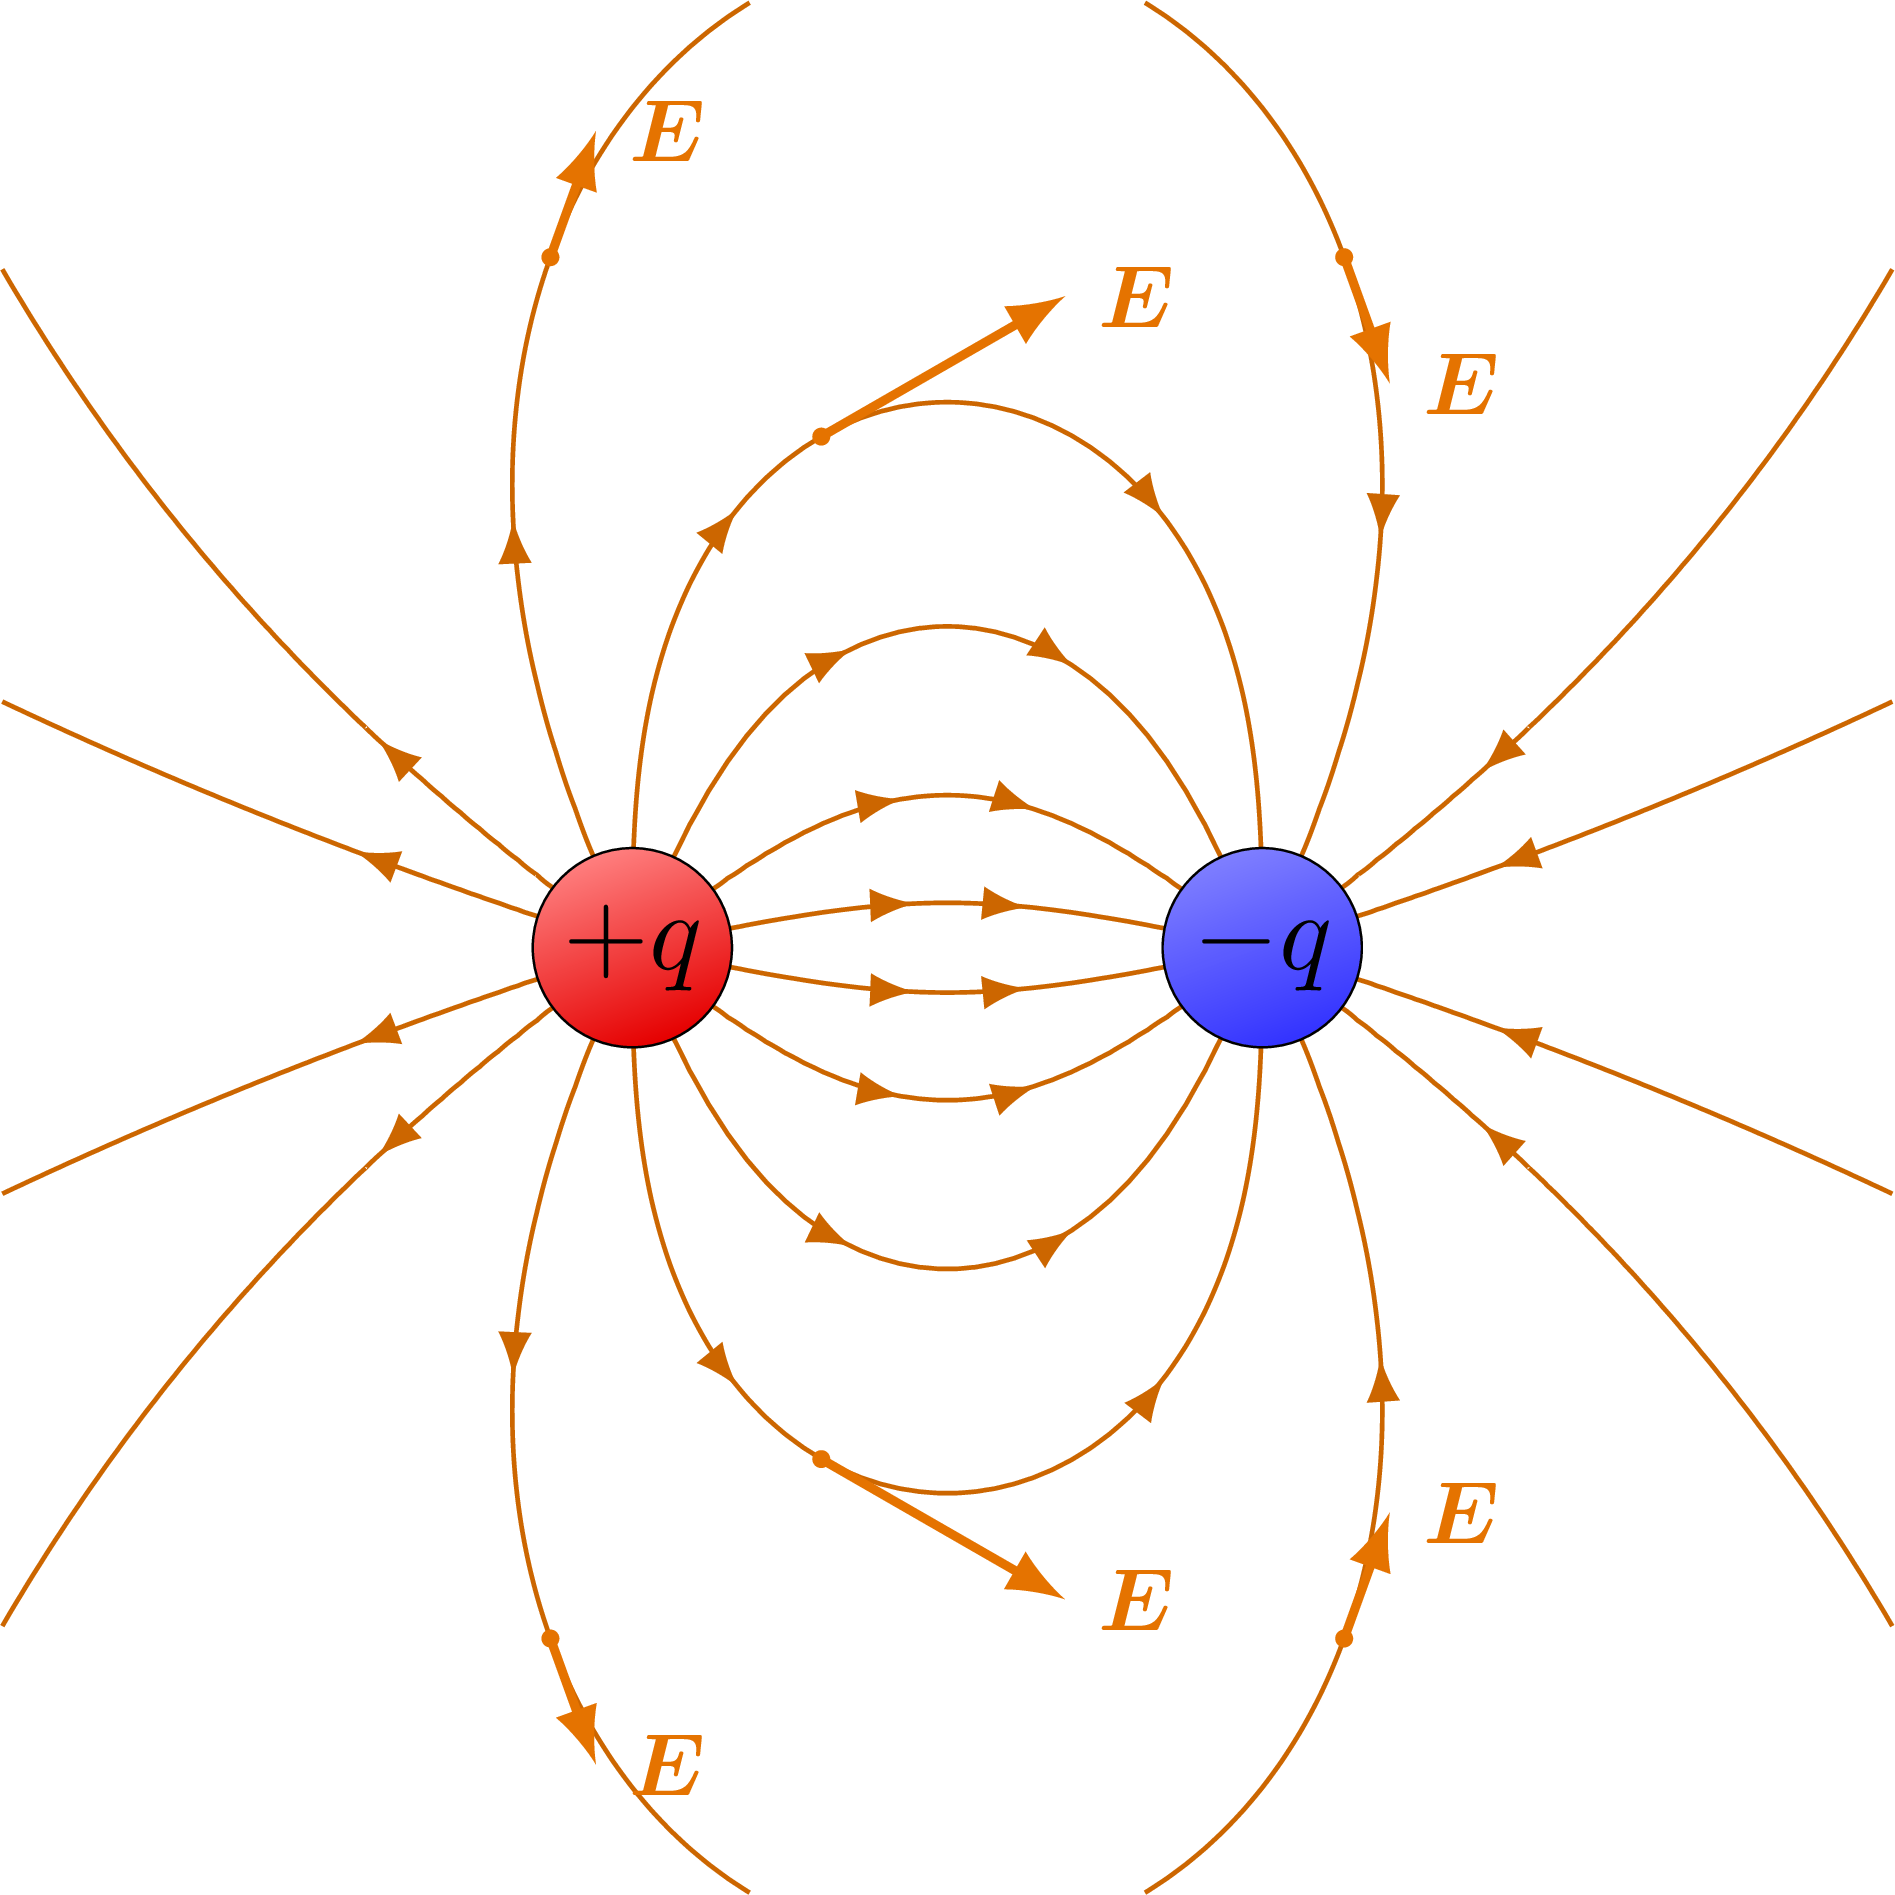
\includegraphics[width = 1\textwidth]{image/interazioneCampiElettrici.png}
      \end{minipage}
     \hspace{0.1mm}
     \begin{minipage}[c]{0.4\textwidth}
        \centering
        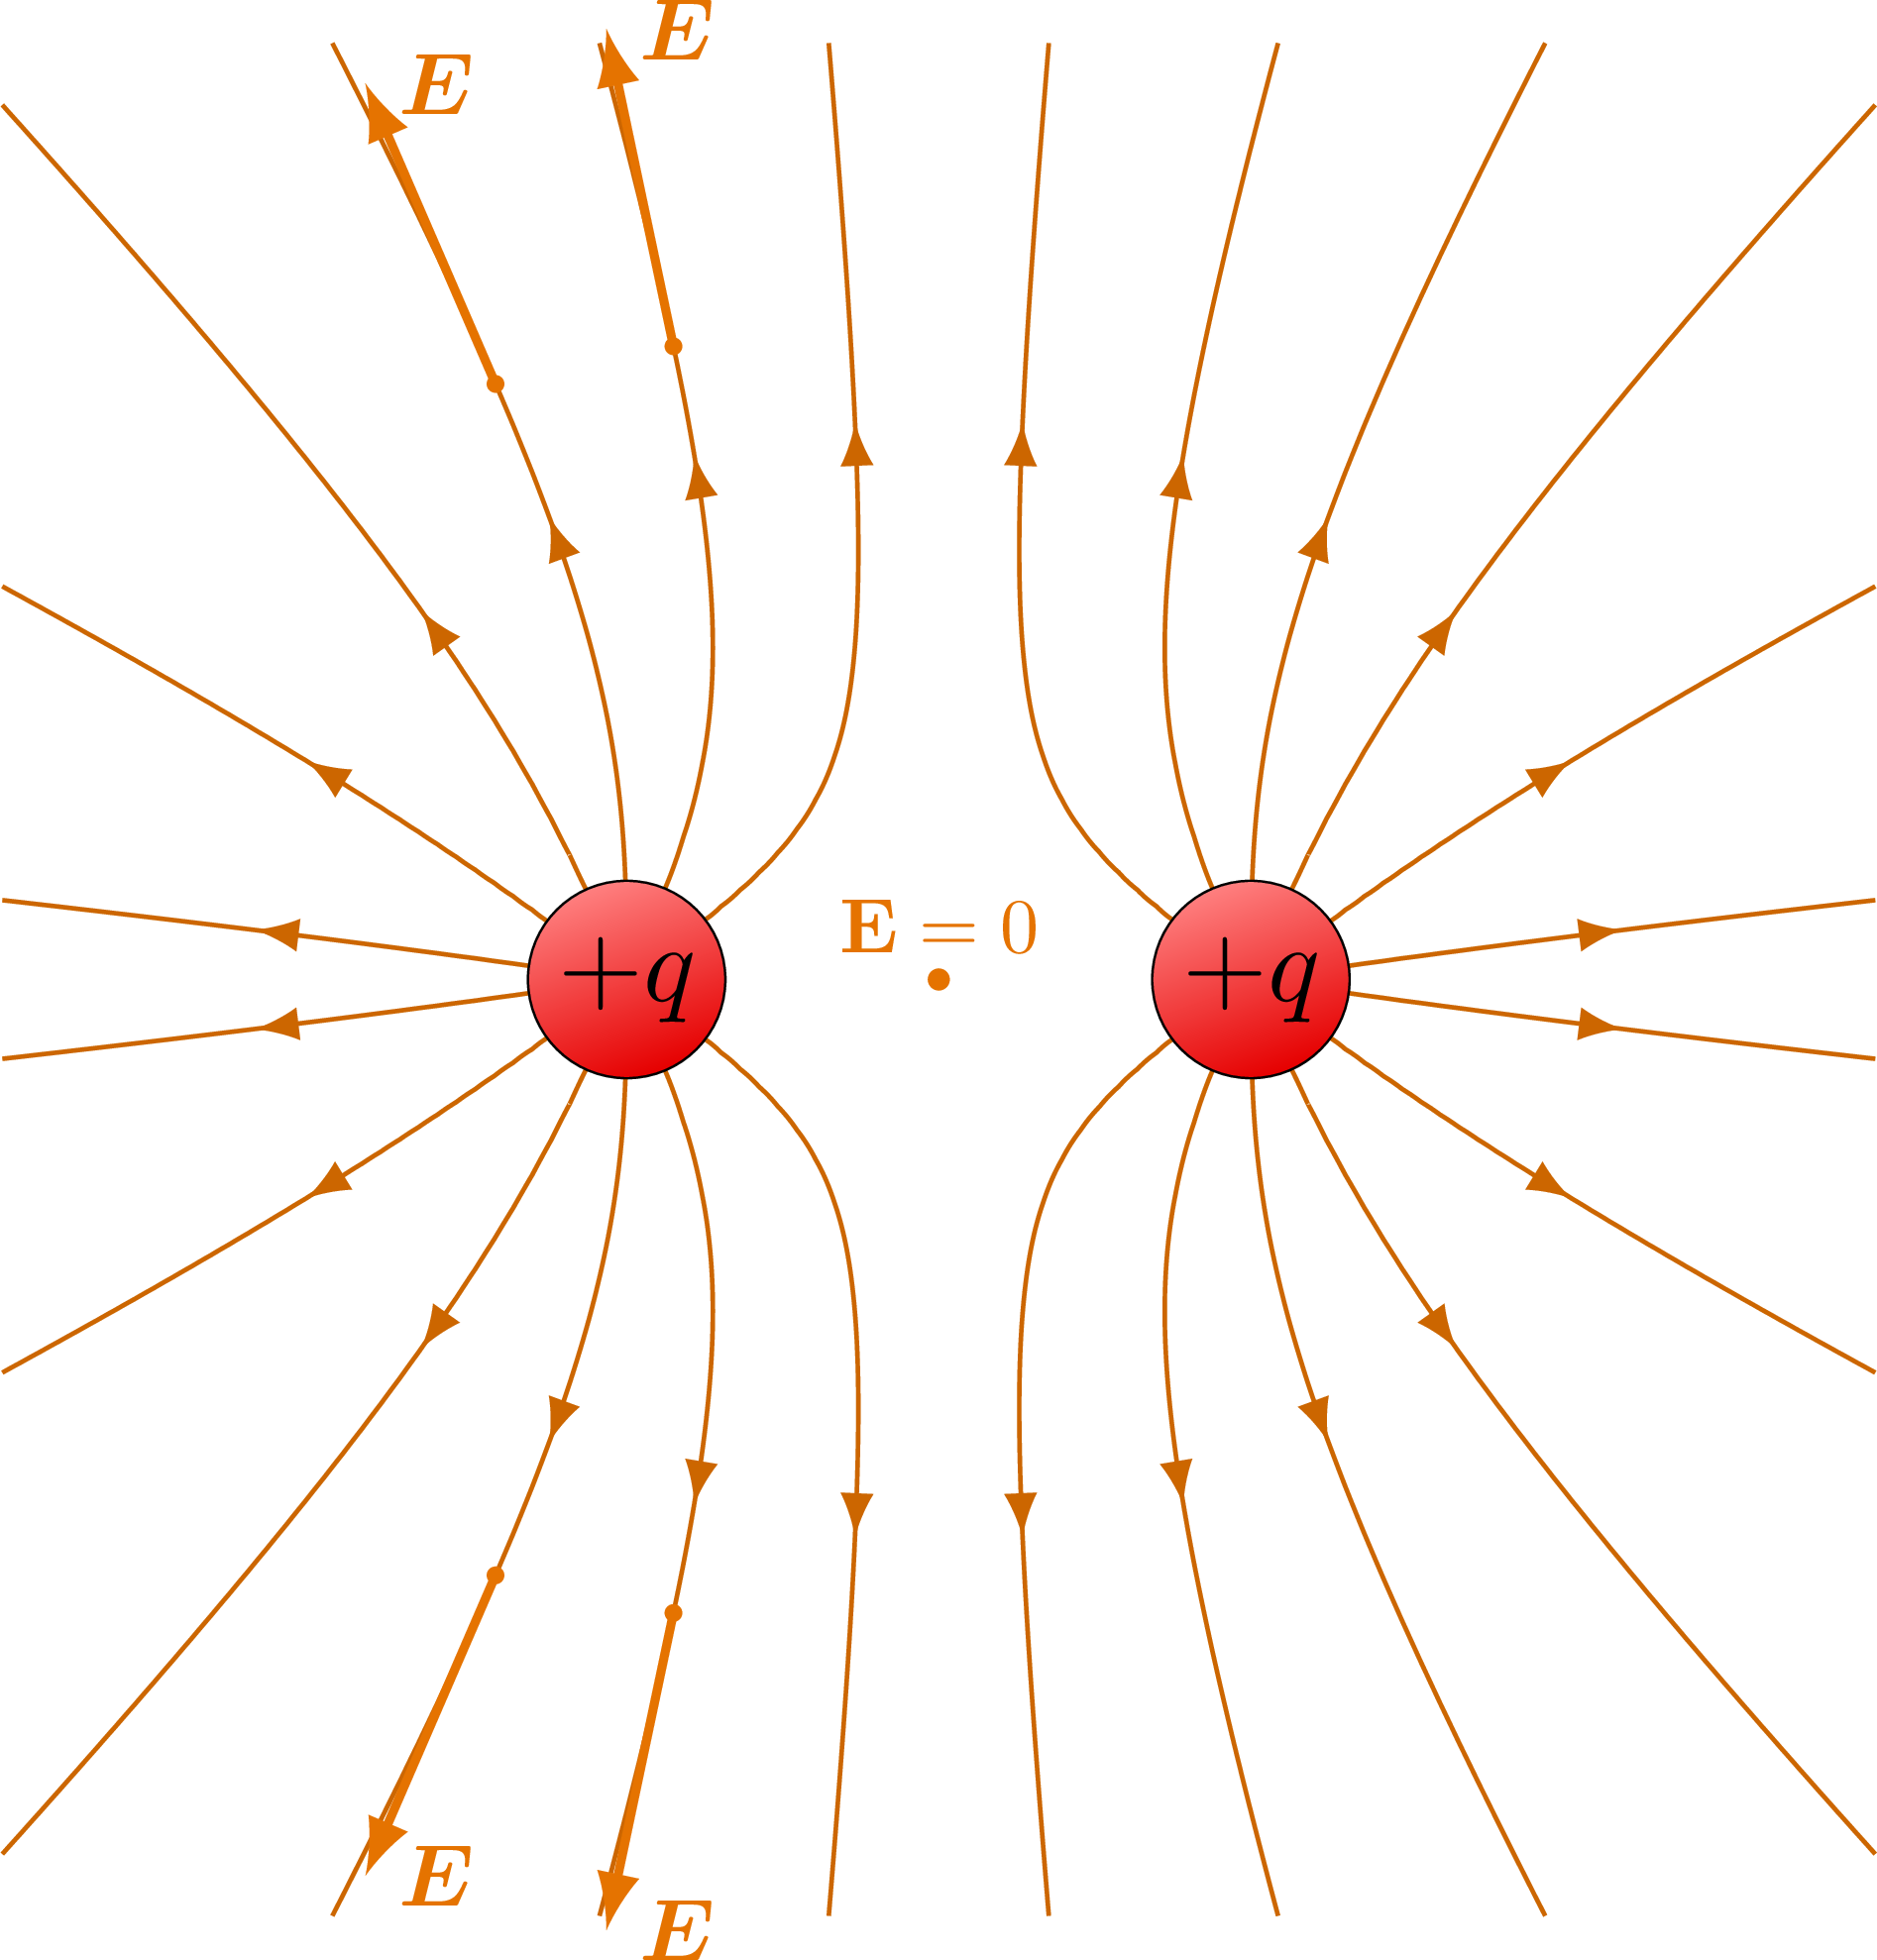
\includegraphics[width = 1\textwidth]{image/interazioniCampiElettrici2.png}
     \end{minipage}
     \caption{Campo elettrico attrattivo a sinistra e repulsivo a destra}
     \label{fig:campoElettricoAttrRep}
 \end{figure}
 
 Per fornire una definizione di campo elettrico consideriamo una carica $Q$. La sola presenza di questa carica modifica attorno ad essa lo spazio circostante, Figura \ref{fig:campoElettricoPosNeg}, e qualsiasi altra carica $Q^*$ che venga introdotta nella regione di spazio in cui agisce il campo generato da $Q$ risentirà di una forza di Coulomb, attraente o repulsiva.
 
 Da qui possiamo allora definire la formula del campo elettrico come:
 
 \begin{equation}
     \vec{E } = \frac{1}{4\pi \varepsilon_0}\frac{Q}{r^2}\vec{u}_r = K_e\frac{Q}{r^2}\vec{u}_r = \frac{\vec{F}}{Q}\qquad\biggl[\frac{N}{C}\biggl]
 \end{equation}
 
 
 \section{Sovrapposizione di campi elettrici}
 Il campo elettrico totale generato da un insieme di cariche in un punto è la
somma vettoriale dei campi elettrici generati da ogni singola carica in quel
punto, dove ciascun campo elettrico va calcolato indipendentemente dagli altri.

La formula per calcolare il campo elettrico totale è la seguente:

\begin{equation}
    \vec{E}_{tot} = \sum_i=1^n \vec{E}_i
\end{equation}

calcolando il modulo del campo elettrico totale avremo:
\begin{equation}
    E_{tot} = K_e\sum_i=1^n \frac{q_i}{r^2}
\end{equation}

\section{Teorema di Gauss per il campo elettrico}
In ogni punto dello spazio attorno a una carica è definito un vettore campo elettrico. L’insieme di questi vettori forma un campo vettoriale che contiene l’informazione relativa alla carica che l’ha creato.

Introduciamo ora una grandezza costituita a partire dal campo elettrico: il \textbf{flusso} attraverso una superficie.

\subsection{Il flusso del campo elettrico}
Il flusso del campo elettrico attraverso una superficie è dato dall'integrale del campo elettrico sulla superficie \footnote{o vettore area} considerata; nel caso di un campo elettrico uniforme e di una superficie piana il calcolo si riduce al prodotto scalare tra il vettore campo elettrico e il vettore superficie.

Per scrivere la definizione di flusso abbiamo bisogno di una superficie limitata nello spazio e un vettore area, il quale ha come modulo l'area e come direzione la retta normale alla superficie nel punto.

\paragraph{}

Il flusso del campo elettrico $\Phi(\vec{E})$ attraverso una superficie qualsiasi esprime, in un certo modo, una misura delle linee di campo elettrico che attraversano la superficie considerata, indipendentemente che sia aperta o chiusa, piana o ricurva.
Supponiamo che $\vec{E}$ sia un campo elettrico uniforme: il suo modulo è costante per ogni punto.

\paragraph{}
Definiamo il flusso del campo elettrico $\vec{E}$ come il prodotto scalare del vettore $\vec{E}$ per il vettore area $\vec{S}$:

\begin{equation}
    \Phi(\vec{E}) = \vec{E}\cdot\vec{S}\qquad\biggl[\frac{N\,m^2}{C}\biggl]
\end{equation}
possiamo scrivere il flusso, essendo un prodotto scalare,  come:
\begin{equation}
    \Phi(\vec{E}) = ES\cos{\theta}
\end{equation}
dove $S$ rappresenta l'area della superficie.
Si può capire che il flusso ha valore massimo quando i vettori campo elettrico sono perpendicolari alla superficie e paralleli al vettore superficie. Mentre assumerà il valore nullo quando la superficie è parallela al campo elettrico.


\def\L{2.2}
\def\H{2.2}
\def\offset{2.0}
\def\W{0.30}
\def\Nx{5}
\def\Ny{5}
\begin{figure}[tb]
    \centering
    
       \begin{tikzpicture}[x={(1.0cm,0)},y={(0.55cm,0.5cm)},z={(0,1.0cm)}]
      \def\H{2.5}
      \def\W{4.8}
      \def\Ny{5}
      \def\Nz{4}
      \def\NEy{4}
      \def\NEz{3}
      \def\oEy{0.08*\W}
      \def\oEz{0.04*\H}
      \def\E{2}
      \coordinate (O) at (0.0,-0.5,-0.5);
      
      % AXES
      \draw[->,thick] (0.5,0,0) --++ (0.5*\H,0,0) node[right] {$x$};
      %\draw[->,thick] (O) --++ (0.5*\H,0,0) node[right] {$x$};
      %\draw[->,thick] (O) --++ (0,0.7*\H,0) node[right] {$y$};
      %\draw[->,thick] (O) --++ (0,0,0.5*\H) node[above] {$z$};
      
      % ELECTRIC FIELD back
      \foreach \i [evaluate={\y=\oEy+(\i-0.5)*(\W-2*\oEy)/\NEy;}] in {1,...,\NEy}{
        \foreach \j [evaluate={\z=\oEz+(\j-0.5)*(\H-2*\oEz)/\NEz;}] in {1,...,\NEz}{
          \draw[EFieldLine,very thick] (0,\y,\z) --++ (-\E,0,0);
        }
      }
      
      % PLANE
      \draw[charged]
        (0,0,0) --++ (0,\W,0) --++ (0,0,\H) --++ (0,-\W,0) -- cycle;
      \foreach \i [evaluate={\y=(\i-0.5)*\W/\Ny;}] in {1,...,\Ny}{
        \foreach \j [evaluate={\z=(\j-0.5)*\H/\Nz;}] in {1,...,\Nz}{
          \node[scale=0.8,rotate=0] at (0,\y,\z) {$+$};
        }
      }
      
      % ELECTRIC FIELD front
      \foreach \i [evaluate={\y=\oEy+(\i-0.5)*(\W-2*\oEy)/\NEy;}] in {1,...,\NEy}{
        \foreach \j [evaluate={\z=\oEz+(\j-0.5)*(\H-2*\oEz)/\NEz;}] in {1,...,\NEz}{
          \draw[EFieldLine,very thick] (0,\y,\z) --++ (\E,0,0);
        }
      }
      \node[Ecol] at (1.3,0.88*\W,0.88*\H) {$\vb{E}$};
     
    \end{tikzpicture}
    \caption{Flusso massimo, il piano è ortogonale al campo elettrico }
    \label{fig:flussoMassimo}

\end{figure}

\section{La legge di Gauss}
\label{teoremaGauss}

Il teorema di Gauss afferma che il flusso di un campo elettrico di una superficie chiusa è dato dal rapporto tra carica elettrica totale interna alla superficie e la costante dielettrica.

\begin{equation}
    \Phi(\vec{E})  =\frac{Q}{\varepsilon_0}
\end{equation}

\subsection{Dimostrazione del teorema di Gauss}
Per dimostrarlo consideriamo una superficie sferica, con una carica puntiforme collocata al centro della sfera.

\def\L{2.2}
\def\H{2.2}
\def\W{0.30}
\def\Nx{5}
\def\Ny{5}
\begin{figure}
    \centering
    \begin{tikzpicture}
      \def\N{7}
      \def\R{2.2}
      \def\r{0.8}
      
      % SPHERE BACK
      \begin{scope}
        \clip (-\R,0) rectangle ++(2*\R,\R);
        \draw[gauss line,very thin,dashed]
          (0,0) ellipse ({\R} and {\r});
      \end{scope}
      
      % CHARGES
      \node[charge+,scale=0.8,circle,inner sep=0.27] (C) at (0,0) {$+Q$};
      
      % FIELD LINES
      \path[name path=ell](0,0) ellipse ({0.78*\R} and {\R});
      \foreach \i [evaluate={\ang=-8+\i*360/\N;}] in {1,...,\N}{
        %\message{Eline\i^^J}
        \draw[EFieldLine,name path global/.expanded=Eline\i] (C) -- ({1.2*\R*cos(\ang)},{1.3*\R*sin(\ang)}) coordinate (E\i);
        %(\ang:1.3*\R)
      }
      
      % SPHERE
      \draw[gauss line,ball color=green!70!black,fill opacity=0.1]
        (0,0) circle (\R);
      \begin{scope}
        \clip (-\R,0) rectangle ++(2*\R,-\R);
        \draw[gauss line,very thin]
          (0,0) ellipse ({\R} and {0.3*\R});
      \end{scope}
      \draw[<->,gauss line,very thin]
        (C) -- (190:{\R} and {\r}) node[measure] {$R$}; %{\contour{green!70!black!7}{$R$}};
      
      % VECTOR
      \draw[gauss dark,name intersections={of={Eline1} and ell,name=ES1}]
        (ES1-1) ++ (-0.081*\R,0.033*\R) to[out=20,in=180] ++(10:0.09*\R)
                                        to[out=-35,in=115] ++(-50:0.09*\R)
                                        to[out=185,in=15] ++(190:0.09*\R)
                                        to[out=120,in=-40] cycle; %node[left] {$\dd{A}$};
      \node[green!40!black,right=5,below=2] at (ES1-1) {$\dd{S}$};
      \foreach \i [evaluate={\angle=8+\i*360/\Nx;}] in {1,6,7}{
        \draw[EField,-,name intersections={of={Eline\i} and ell,name=ES\i}] (ES\i-1) -- (E\i);
      }
      \draw[normalvec] (ES1-1) ++ (138:0.03*\R) --++ (50:0.16*\R) node[above=-1] {$\vec{s}$};
      
    \end{tikzpicture}
    \caption{Carica puntiforme nel centro della sfera}
    \label{fig:caricaPuntiformeGauss}
\end{figure}


Siccome la carica interna è positiva, le linee di campo sono uscenti, dunque tale è anche il verso di $\vec{E}$.

Se cercassimo ora di dividere la superficie sferica in tantissime parti, otterremo tante superfici infinitesime $dS$ che inevitabilmente risulteranno una superficie piana in cui il campo su ciascuna superficie infinitesima possa essere considerato uniforme. Questo ragionamento è applicabile a qualsiasi superficie chiusa $S$, detta superficie gaussiana, immersa in un campo elettrico.

Il flusso totale del campo elettrico sarà dato dalla somma di tutti i contributi delle superfici infinitesime $dS$ della sfera.
Visto che stiamo considerando una superficie infinitesima, anche il relativo contributo del flusso deve essere infinitesimo e dunque scriveremo:

\begin{equation*}
    d\Phi = \vec{E}\cdot d\vec{S}
\end{equation*}

tale prodotto scalare diventa:

\begin{equation*}
    d\Phi = Eds\cos{0} = EdS
\end{equation*}

per ottenere la somma di tutti i flussi infinitesimi dobbiamo integrare su tutta la superficie, dunque:

\begin{equation*}
    \Phi(\vec{E}) = \oint_s \vec{E}\cdot d\vec{S} = \int_s d\Phi = \int_s Eds
\end{equation*}
Essendo una superficie piana il campo elettrico è costante e si può portare fuori dall'integrale:
\begin{equation*}
    \Phi(\vec{E})  = E\int_s ds  = ES
\end{equation*}

nel nostro caso la superficie $S$ si tratta di una superficie sferica e, a questo punto,  sostituendo ci siamo ricondotti al teorema di Gauss:

\begin{equation}
    \Phi(\vec{E}) = \frac{1}{4\pi\varepsilon_0}\frac{Q}{r^2}4\pi r^2 = \frac{Q}{\varepsilon_0}
\end{equation}

\paragraph{}
Risolvendo l'equazione del teorema di Gauss otteniamo:
\begin{equation*}
     \Phi(\vec{E}) = \frac{Q}{\varepsilon_0}
\end{equation*}

\begin{equation*}
     \oint_s \vec{E}\cdot d\vec{S} = \frac{Q}{\varepsilon_0}
\end{equation*}

\begin{equation*}
     E\int_s dS = \frac{Q}{\varepsilon_0}
\end{equation*}

la superficie di una sfera è $4\pi r^2$ e dunque:
\begin{equation*}
    \Phi(E) = E4\pi r^2
\end{equation*}
\begin{equation*}
     E4\pi r^2 = \frac{Q}{\varepsilon_0}
\end{equation*}

\begin{equation*}
     E = \frac{Q}{4\pi\varepsilon_0r^2}
\end{equation*}

possiamo capire ora che la legge di Coulomb è una conseguenza del teorema di Gauss.



\section{Campo elettrico cavo infinito}
\label{paginaCampoElettricoCavoInfinito}


\def\L{8}
\def\W{0.25}
\def\N{14}
\def\M{4}
 \def\ymax{\L/3}
\begin{figure}[H]
    \centering
    \begin{tikzpicture}[rotate = -90, scale = 0.8]
      \def\R{0.4*\L}
      \def\g{0.2*\R}
      \def\G{0.6*\R}
      \def\a{0.33*\L}
      \coordinate (L)  at (-\a,0);
      \coordinate (R)  at (+\a,0);
      \coordinate (TL) at (-\a,\G);
      \coordinate (TR) at (+\a,\G);
      \coordinate (BL) at (-\a,-\G);
      \coordinate (BR) at (+\a,-\G);
      
      % GAUSS BEHIND
      \draw[gauss line,dashed] (TR) arc (90:270:{\g} and {\G});
      
      % ROD
      \draw[charged] (-\L/2,-\W/2) --++(\L,0) to[out=0,in=0] ++ (0,\W) --++ (-\L,0) -- cycle;
      \draw[charged] (-\L/2,-\W/2) to[out=180,in=180] ++ (0,\W) to[out=0,in=0] cycle;
      \foreach \i [evaluate={\x=-\L/2+\i*\L/(\N+1);}] in {1,...,\N}{
        \node[scale=0.6] at (\x,0) {$+$};
      }
      \begin{scope}
        \clip (-\L/2,-0.5*\W)
          --++ (\L/2-\a,0) to[out=50,in=-50] ++(0,1.0*\W) --++ (-\L/2+\a,0) --++ (0,\G)
          --++ (\L-2*\a,0) --++ (0,{-2*(\G+\W)}) --++ (-\L+2*\a,0) -- cycle;
        \draw[gauss lid] (L) ellipse ({\g} and {\G});
      \end{scope}
      
      
      % GAUSS IN FRONT
      \draw[<->] (-\a,-\W/2) -- (-\a,-\G) node[measure,fill=green!80!black!8,inner sep=1,outer sep=0] {$r$};
      \draw[<->] (-\a,-1.1*\G) -- (\a,-1.1*\G) node[measure] {$L$};
      \draw[gauss surf]
        (BL) arc (-90:90:{\g} and {\G}) --
        (TR) arc (90:-90:{\g} and {\G}) -- cycle;
      \draw[normalvec] (-0.064*\L,\G) --++ (0,0.25*\G) node[left=2,above] {$\vu{n}$};
      \draw[->,thick,Ecol] (-0.045*\L,\G) --++ (0,0.6*\G) node[right] {$\vb{E}$};
      
      \draw[->,thick,Ecol] (-\a,1) --++ (0,2.08) node[right] {$\vb{E}$};
      
      % LABELS
      \node[left,green!30!black] at ($(-\a,0)+(150:{\g} and {\G})$) {$S_1$};
      \node[right,green!30!black] at ($(\a,0)+(30:{\g} and {\G})$) {$S_2$};
      \node[above,green!30!black] at (0.6*\a,\G) {$S_3$};
      
  
    \end{tikzpicture}
    \caption{Campo elettrico attorno ad un filo infinito}
    \label{fig:campoElettFiloInf}
\end{figure}



Con questo esempio vogliamo studiare quale sia il flusso che attraversa il cilindro.
Sappiamo che il flusso totale ha la seguente formula:

\begin{equation*}
    \Phi_t(E) = E\int_{sup. lat.}dS
\end{equation*}
la superficie esterna del cilindro la sappiamo calcolare e dunque il flusso sarà:
\begin{equation*}
    \Phi(E) = E2\pi rh
\end{equation*}
\begin{equation*}
    E2\pi rh = \frac{\lambda h}{\varepsilon_0}
\end{equation*}
\begin{equation}
    E = \frac{\lambda}{2\pi r\varepsilon_0}  = \frac{\rho_{0}\pi r^2}{2\pi r\varepsilon_0}
    \label{leggeDiGaussDim}
\end{equation}

Dove $\lambda\,[\frac{C}{m}]$ indica la densità di carica nel filo.
\paragraph{}
Sulle basi $S_1$ e $S_2$ il campo elettrico è parallelo alla base e il prodotto \\$\vec{E}\cdot d\vec{s} = Edscos\theta$ è nullo in quanto il coseno è zero.
 
\section{Piano infinito}
\label{pianoInfinito}

\begin{figure}[H]
    \centering
    \begin{tikzpicture}[x={(1.0cm,0)},y={(0.55cm,0.5cm)},z={(0,1.0cm)}, scale = 1.3]
      \def\H{2.5}
      \def\W{4.8}
      \def\Ny{5}
      \def\Nz{4}
      \def\R{0.14*\W}
      \def\a{0.49*\H}
      \def\E{0.36*\H}
      \def\plane{(0,0,0) --++ (0,\W,0) --++ (0,0,\H) --++ (0,-\W,0) -- cycle;}
      \coordinate (O) at (0.0,-0.5,-0.5);
      \coordinate (C)  at (      0,\W/2,\H/2);
      \coordinate (ER) at (     \a,\W/2,\H/2);
      \coordinate (EL) at (-1.2*\a,\W/2-0.6*\R,\H/2+0.5*\R);
      \coordinate (TM) at (      0,\W/2,\H/2+\R);
      \coordinate (TR) at (     \a,\W/2,\H/2+\R);
      \coordinate (TL) at (-1.2*\a,\W/2,\H/2+\R);
      \coordinate (BM) at (      0,\W/2,\H/2-\R);
      \coordinate (BR) at (     \a,\W/2,\H/2-\R);
      \coordinate (BL) at (-1.2*\a,\W/2,\H/2-\R);
      \coordinate (NT) at (0.7*\a,\W/2,\H/2+\R);
      \coordinate (NR) at (\a,\W/2+0.13*\R,\H/2+0.13*\R);
      \coordinate (NL) at (-1.2*\a,\W/2-0.5*\R,\H/2-0.2*\R);
      \coordinate (NB) at (0.86*\a,\W/2-0.6*\R,\H/2-0.6*\R);
      
      % AXES
      \draw[->,thick] (0.5,0,0) --++ (0.5*\H,0,0) node[right] {$x$};
      
      % VECTORS back
      \draw[EField] (EL) --++ (-\E,0,0);
      \draw[normalvec] (EL) ++(0,-0.1*\R,-0.13*\R) --++ (-0.5,0,0) node[below left=-4] {$\vu{n}$};
      \draw[gauss dark]
        (EL)++(0,-0.1*\R,-0.3*\R)
          to[out=0,in=0,looseness=1.2] ++(0,0,0.5*\R)
          to[out=180,in=180,looseness=1.2] ++(0,0,-0.5*\R) -- cycle; %node[left=4,below=-1] {$\dd{A}$};
      
      % GAUSSIAN SURFACE back
      \draw[gauss dashed line] (BL) to[out=0,in=0,looseness=1.2] (TL);
      \draw[gauss surf]
        (BM) to[out=180,in=180,looseness=1.2] (TM) --
        (TL) to[out=180,in=180,looseness=1.2] (BL) -- cycle;
      
      % PLANE
      \draw[charged] \plane;
      \begin{scope}
        \clip \plane;
        \draw[gauss dashed line] (BM) -- (BL);
        \draw[gauss dashed line] (TM) -- (TL);
        \draw[gauss dashed line] (BL) to[out=0,in=0,looseness=1.2] (TL);
      \end{scope}
      \foreach \i [evaluate={\y=(\i-0.5)*\W/\Ny;}] in {1,...,\Ny}{
        \foreach \j [evaluate={\z=(\j-0.5)*\H/\Nz;}] in {1,...,\Nz}{
          \node[scale=0.8,rotate=0] at (0,\y,\z) {$+$};
        }
      }
      \draw[gauss dark]
        (NT) ++ (-0.12,0,0) to[out=-5,in=110] ++(0,0.12,-0.10) --++(0.22,0,0) to[out=110,in=-5] ++(0,-0.12,0.10) -- cycle;
      
      % GAUSSIAN SURFACE front
      \draw[gauss dashed line]
        (BM) to[out=0,in=0,looseness=1.2] (TM);
      \draw[gauss surf]
        (BM) to[out=180,in=180,looseness=1.2] (TM) --
        (TR) to[out=180,in=180,looseness=1.2] (BR) -- cycle;
      \draw[gauss lid]
        (BR) to[out=0,in=0,looseness=1.2] (TR) to[out=180,in=180,looseness=1.2] cycle;
      
      % DARK
      \draw[gauss dark]
        (NT) ++ (-0.12,0,0) to[out=-160,in=80] ++(0,-0.12,-0.05) --++(0.22,0,0) to[out=80,in=-160] ++(0,0.12,0.05) -- cycle;
      \draw[gauss dark]
        (ER)++(0,0.1*\R,-0.2*\R)
          to[out=0,in=0,looseness=1.2] ++(0,0,0.5*\R)
          to[out=180,in=180,looseness=1.2] ++(0,0,-0.5*\R) -- cycle node[left = -3, below=-3] {$\dd{A}$};
      
      % ELECTRIC FIELD
      \draw[EField] (ER) --++ (\E,0,0) node[right] {$\vb{E}$};
      \draw[EField] (NT) --++ (\E,0,0) node[right] {$\vb{E}$};
      
      % VECTORS
      \draw[normalvec] (ER) ++(0,0.1*\R,0.13*\R) --++ (0.5,0,0) node[above=3,right=-2] {$\vu{n}$};
      \draw[normalvec] (NT) --++ (0,0,0.5) node[below=1,left=-1] {$\vu{n}$};
      %\draw[normalvec] (NB) --++ (0,-0.35,-0.25) node[below right=-2] {$\vu{n}$};
      
      
    \end{tikzpicture}
    \caption{Piano infinito}
    \label{fig:pianoInfnito}
\end{figure}
 
Con questo esempio vogliamo studiare quale sia il flusso che attraversa il cilindro.
Sappiamo che il flusso totale ha la seguente formula:

\begin{equation*}
    \Phi_t(E) = E\int_{base 1}dS + E\int_{base 2}dS
\end{equation*}
la superficie esterna del cilindro la sappiamo calcolare e dunque il flusso sarà:
\begin{equation*}
    \Phi(E) = E2\pi r^2
\end{equation*}
\begin{equation*}
    E2\pi r^2 = \frac{\sigma}{\varepsilon_0}
\end{equation*}
\begin{equation}
    E = \frac{\sigma}{2\varepsilon_0}
\end{equation}

Dove $\sigma \frac{C}{m^2}$ indica la densità di carica nel piano.

\section{Calcolare il campo elettrico ad una distanza arbitraria da un filo}

\begin{figure}[H]
    \centering
    \begin{tikzpicture}[scale = 1, rotate = -90]
          \def\xmax{0.6*\L}
          \def\ymin{-0.18*\L}
          \def\ymax{0.5*\L}
          \def\x{0.342*\L}
          \def\dx{0.05*\L}
          \coordinate (O) at (0,0);
          \coordinate (P) at (0,{0.6*\ymax});
          \coordinate (X) at (\x,\W/2);
          
          % AXIS
          \draw[->,thick] (\xmax, 0) -- (-\xmax,0) node[left] {$y$};
          \draw[->,thick] (0,\ymin) -- (0,\ymax) node[below] {$x$};
          
          % MEASURES
          %\draw[<->] (0,0.2*\ymax) --++ (\x,0) node[midway,above] {$x$};
          \draw[<->] (    0,0.25*\ymin) --++ (\x,0) node[measure] {$y$};
          \draw[<->] (   \x,0.25*\ymin) --++ (\dx,0) node[midway,left] {$dy$};
          \draw[<->] (-\L/2,0.62*\ymin) --++ (\L,0) node[measure, below = 10] {$L$};
          
          % VECTORS
          \draw[EField,very thick] (P) --++ ( 0.0,0.6) node[right=7, below] {$\dd{\vb{E}_x} = \vec{j}\cos\theta$};
          \draw[EField,very thick] (P) --++ (-0.6,0.0) node[left=-1] {$\dd{\vb{E}_y} = \vec{j}\sin\theta$};
          \draw[EField,very thick] (P) --++ (-0.6,0.6) node[above left=-2] {$\dd{\vb{E}}$};
          \draw[EField,-,dashed,thin] (P) ++ (0,0.6) --++ (-0.6,0) --++ (0,-0.6);
          
          % POINT
          \fill (P) circle (0.06) node[below=8,right=1] {P};
          \draw[<->] (-0.25,0.2) --++ (0,2.1) node[measure] {$r$};
          \draw[dashed] (P) -- (X) node[measure]{$R$};
          \draw pic[->,"$\theta$",draw=black,angle radius=20,angle eccentricity=1.4] {angle = O--P--X};
          \draw[vector] (X) -- ($(X)!0.12!(P)$) node[above] {$\vu{r}$};
          
          % ROD
          \draw[charged] (-\L/2,-\W/2) rectangle ++(\L,\W);
          \draw[darkcharged] (\x,-\W/2) rectangle ++(\dx,\W)
            node[above, right] {$\dd{q}=\lambda \dd{x}$};
          \foreach \i [evaluate={\x=-\L/2+\i*\L/(\N+1);}] in {1,...,\N}{
            \node[scale=0.6] at (\x,0) {$+$};
          }

    \end{tikzpicture}
    \caption{Campo elettrico ad una distanza $R$ da un filo}
    \label{fig:campoElettDistanzaRFilo}
\end{figure}

Prendendo un pezzo di filo rettilineo, vogliamo studiare cosa succede in un suo pezzo; il filo può essere anche asimmetrico.

Utilizzando la legge di Coulomb, che non dipende dalle simmetrie, possiamo ricavarci il campo elettrico infinitesimo generato in ogni punto e sommare, con un integrale, tutti i punti del filo:

\begin{equation*}
    d\vec{E}  = \frac{1}{4\pi \varepsilon_0}\frac{dq}{R^2}\hat{r}
\end{equation*}
indichiamo con $dq$ la carica infinitesima del filo data dal rapporto infinitesimo $\lambda = \frac{dq}{dy}$ e $\hat{r}$ il versore diretto dalla carica  verso il punto $P$.

Prendendo un pezzo infinitesimo di filo, $dx$

Sapendo che il campo infinitesimo è dato da:
\begin{equation*}
    d\vec{E} = d\vec{E_x}\vec{i} + d\vec{E_j}\vec{j}
\end{equation*}

Per calcolare il campo elettrico in $P$ dobbiamo servirci degli integrali e dunque:
\begin{equation*}
   \int d\vec{E} = \int d\vec{E_x}\vec{i} + \int d\vec{E_j}\vec{j}
\end{equation*}
\begin{equation*}
   \int_L \frac{1}{4\pi \varepsilon_0}\frac{dq}{R^2}\hat{r}
\end{equation*}

Notiamo che $dy$, $R^2$ e $\hat{r}$ dipendono dalla posizione $y$. Dobbiamo cercare di scrivere tutto in funzione di una singola variabile.

La variabile che più si addice a tale scopo è: $\theta$, l'angolo che viene formato dal punto $dy$ al punto in cui vogliamo calcolare il campo, $P$.

\begin{equation*}
    \frac{y}{r} = \tan\theta\quad\rightarrow\quad y = r\tan\theta
\end{equation*}

\begin{equation*}
     dy = \frac{dy}{d\theta}d\theta
\end{equation*}
deriviamo $y$ trovata prima rispetto a $\theta$ per trovare la nuova variabile di integrazione:
\begin{equation*}
     dy = r\frac{d\theta}{\cos^2\theta}d\theta
\end{equation*}

infine:

\begin{equation*}
    r = r\cos\theta\quad\rightarrow\quad R = \frac{r}{\cos\theta}
\end{equation*}

ora tutte le parti variabili sono funzioni della stessa parte variabile: l'angolo.

Ora possiamo sommare 
\begin{equation*}
    \int_{\theta_1}^{\theta_2} \frac{1}{4\pi \varepsilon_0}\frac{\lambda r d\theta}{\cos^2\theta}\frac{\cos^2\theta}{r^2}[\cos\theta\vec{i} - \sin\theta\vec{j}]
\end{equation*}

\begin{equation*}
    \frac{\lambda}{4\pi \varepsilon_0 r} \biggl[\biggl( \int_{\theta_1}^{\theta_2} \cos\theta d\theta \biggl)\vec{i} + \biggl(\int_{\theta_1}^{\theta_2} -\sin\theta d\theta \biggl)\vec{j}\biggl]
\end{equation*}

\paragraph{}
Risolvendo troviamo che il campo elettrico nel punto $P$ è:
\begin{equation}
    \vec{E}_{(p)}  = \frac{\lambda}{4\pi \varepsilon_0 r}[(\sin\theta_2 - \sin\theta_1)\,\vec{i}\,  + (\cos\theta_2 - \cos\theta_1)\,\vec{j}\,]
\end{equation}

\paragraph{}
Alcune considerazioni finali...\\
se il filo lo metto in modo tale da avere una simmetria rispetto l'asse $y$ allora l'equazione diventa:

\begin{equation}
    \vec{E}_{(p)}  = \frac{\lambda}{4\pi \varepsilon_0 r}[(\sin\theta_2 - \sin\theta_1)\,\vec{i}\,]
\end{equation}

\paragraph{Se il filo fosse infinito?}
Se il filo fosse infinito avremo che $\theta = \frac{\pi}{2}$

\begin{equation*}
    \vec{E}_{(p)} = \frac{\lambda}{4\pi \varepsilon_0 r}[1-(-1)\,\vec{i}\,] = \frac{\lambda}{2\pi \varepsilon_0 r}\vec{i}
\end{equation*}

e questo segue la dimostrazione del teorema di Gauss, Pagina \pageref{paginaCampoElettricoCavoInfinito}.

\section{Disco}


\begin{figure}[H]
    \centering
    \begin{tikzpicture}[x={(1,0)},y={(0,0.5)}, scale = 1.3]
      \def\R{2.6}
      \def\r{1.35}
      \def\dr{0.52}
      \def\Ex{0.6}
      \def\Ey{1.1}
      \def\Nx{4}
      \coordinate (O) at (0,0);
      \coordinate (P) at (0,4.0);
      \coordinate (Y) at (0,6.0);
      \coordinate (R) at (\r,0);
      
      % PLANE
      \draw[charged]
        (O) circle (\R);
      \draw[darkcharged,even odd rule]
        (O) circle (\r+\dr) circle (\r);
      \foreach \i [evaluate={\cr=(\i-0.5)*\R/\Nx; \Ny=7+4*(\i-2);}] in {1,...,\Nx}{
        \foreach \j [evaluate={\cang=39+\j*360/\Ny;}] in {1,...,\Ny}{
          \node[scale=0.8,rotate=0] at (\cang:\cr) {$+$};
        }
      }
      
      % CHARGE
      \node[right=-1.5,scale=0.9] at (4:\r+\dr) {$\dd{q}=\sigma \dd{S}$};
      
      % AXIS
      \draw[->,thick] (0,0) -- (Y) node[above] {$z$};
      
      % VECTORS
      \draw[EField,very thick] (P) --++ ( 0.0,\Ey) node[right=1] {$\dd{\vb{E}_y}$};
      \draw[EField,very thick] (P) --++ (-\Ex,0.0) node[left=2] {$\dd{\vb{E}_x}$};
      \draw[EField,very thick] (P) --++ (-\Ex,\Ey) node[above left=-2] {$\dd{\vb{E}}$};
      \draw[EField,-,dashed,thin] (P) ++ (0,\Ey) --++ (-\Ex,0) --++ (0,-\Ey);
      \node[fill=blue!60!black,circle,inner sep=1.1] (P') at (P) { };
      \node[above=3,right=1] at (P') {P};
      \draw[vector,veccol] (R) -- (P') node[pos=0.8,right=3] {$\vb{L}$};
      \draw[vector,veccol] (0,0) --++ (0:\r) node[pos=0.7,above=-1] {$\vb{r}$};
      \draw[<->] (0,0) --++ (-101:\R) node[pos=0.35,right=-2] {$R$};
      
      \draw[->,thick] (-3,-3) --++ (6,6) node[right = 3] {$y$};
      \draw[->,thick] (-3,3) --++ (6,-6) node[right = 3] {$x$};
      
      
    \end{tikzpicture}
    \caption{Disco infinito}
    \label{fig:discoInfinito}
\end{figure}

ogni superficie infinitesima è:
\begin{equation*}
    dq = \sigma ds = \sigma rd\theta dr
\end{equation*}

\begin{equation*}
    d\vec{E_z} = \int_{disco} \frac{1}{4\pi \varepsilon_0}\frac{dq}{r'}\cos\alpha \vec{k}
\end{equation*}
$\vec{k}$ è il versore dell'asse z

\begin{equation*}
   \frac{\sigma h 2\pi}{4 \pi \varepsilon_0}\int_0 ^R (h^2+r^2)^{-\frac{3}{2}} rdr
\end{equation*}

Ora per sommare tutte le piastrelline, i contributi, devo prima sommarle tutte sulla medesima circonferenza e poi sommare tutte le circonferenze per ottenere il disco.

\begin{equation*}
   \int_{0_{(\theta)}} ^ {2\pi} \int_{0_{(r)}} ^ {R} \frac{1}{4\pi \varepsilon_0}\frac{\sigma dr rd\theta}{(h^2 + r^2)}\frac{h}{(h^2 + r^2)^\frac{1}{2}} \vec{K}
\end{equation*}
\begin{equation*}
   \frac{\sigma h 2\pi}{4 \pi \varepsilon_0}\int_0 ^R (h^2+r^2)^{-\frac{3}{2}} rdr
\end{equation*}
\begin{equation*}
   \frac{\sigma h}{2\varepsilon_0} \frac{1}{2}\int_0 ^R (h^2+r^2)^{-\frac{3}{2}} 2rdr
\end{equation*}
\begin{equation*}
   \frac{\sigma h}{2\varepsilon_0} \frac{1}{2}\int_0 ^R (h^2+r^2)^{-\frac{3}{2}} d(r^2)
\end{equation*}
\begin{equation*}
   \frac{\sigma h}{2\varepsilon_0} \frac{1}{2} \biggl[ \frac{(h^2+r^2)}{-\frac{1}{2}} \biggl]_0 ^R
\end{equation*}

\begin{equation*}
   \frac{\sigma h}{2\varepsilon_0} [ -(h^2+ R^2)^{-{\frac{1}{2}}} + h^{-1}]
\end{equation*}
\begin{equation}
   \vec{E} = \frac{\sigma}{2\varepsilon_0} \bigg[ 1 - \frac{h}{\sqrt{h^2 + R^2}}\bigg]\vec{K}
\end{equation}

\paragraph{Cosa ottengo se il disco fosse infinito?}
Se il disco fosse infinito devo ottenere il medesimo risultato che ottengo con Gauss per un piano infinito.

Se il disco diventa infinito, allora $R$ tende a infinito e dunque:
\begin{equation}
    \vec{E} = \frac{\sigma}{2\varepsilon_0} [ 1 - 0] = \frac{\sigma}{2\varepsilon_0}
\end{equation}

ed infatti è proprio lo stesso risultato che otteniamo con un piano infinito, Pagina \pageref{pianoInfinito}.

\paragraph{Se il raggio del cilindro lo tendiamo a zero, ovvero ad un punto?} 
Dovrebbe restituire proprio la legge di Coulomb.
\begin{equation*}
    \vec{E} = \frac{\sigma}{2\varepsilon_0} [ 1 - 1] = \frac{\sigma}{2\varepsilon_0}
\end{equation*}
\begin{equation}
    \vec{E} = 0
\end{equation}

Ma questo non è vero perché far tendere a zero un disco significa anche mandare a zero la sua carica. Nel nostro caso invece la carica la vogliamo mantenere inalterata.
\paragraph{}
Quindi cerchiamo di scriverla in modo diverso:

\begin{equation*}
   \vec{E} = \frac{\sigma}{2\varepsilon_0} \bigg[ 1 - \frac{h}{\sqrt{h^2 + R^2}}\bigg]\vec{K}
\end{equation*}
\begin{equation*}
    \vec{E} = \frac{\sigma}{2\varepsilon_0} \Biggl[ 1 - \frac{h}{h\sqrt{1 + \frac{R^2}{h^2} }}\Biggl]\vec{K}
\end{equation*}
\begin{equation*}
    \vec{E} = \frac{\sigma}{2\varepsilon_0} \Biggl[ 1 - \frac{1}{\sqrt{1 + \frac{R^2}{h^2} }}\Biggl]\vec{K}
\end{equation*}

Ora per trovare la soluzione corretta dobbiamo utilizzare lo sviluppo di Taylor applicato a: 

\begin{equation*}
    f(x) = \frac{1}{\sqrt{1 - x}} = (1-x)^{-\frac{1}{2}} = f(0) + f'(0)x + f''(0)x^2 + \dots
\end{equation*}
\begin{equation*}
    f'(x) = -\frac{1}{2}(1-x)^{-\frac{3}{2}}
\end{equation*}

arrestandoci al $1 \gradi$ ordine otteniamo che:

\begin{equation*}
    f(x) = \frac{1}{\sqrt{1 - x}} = 1 - \frac{1}{2}x
\end{equation*}

Quindi il campo lo riscriviamo come:

\begin{equation*}
    \vec{E} = \frac{\sigma}{2\varepsilon_0 } \Biggl[ 1 - 1 + \frac{1}{2}x\Biggl]\vec{K}
\end{equation*}
sostituendo $x$
\begin{equation*}
    \vec{E} = \frac{\sigma}{2\varepsilon_0} \Biggl[ 1 - 1 + \frac{1}{2}\frac{R^2}{h^2}\Biggl]\vec{K}
\end{equation*}

\begin{equation*}
    \vec{E} = \frac{\sigma R^2 \pi}{ \pi 2\varepsilon_0 2 h^2}
\end{equation*}
moltiplicando sopra e sotto per $\pi$ otteniamo che a numeratore abbiamo $\sigma$ per la superficie del disco $\pi R^2$ che corrisponde alla carica Q.

\begin{equation*}
    \vec{E} = \frac{Q}{ 4 \pi \varepsilon_0  h^2}
\end{equation*}

E questa è la legge di Coulomb.
L'errore è proporzionale alla variabile stessa, infatti continuando la serie di Taylor otteniamo che i termini di grado superiore al primo vanno a zero più rapidamente.


\section{Campo elettrico di una sfera dielettrica}

\begin{figure}[H]
    \centering
    \begin{minipage}[c]{0.4 \textwidth}
    \centering
          \begin{tikzpicture}[scale = 1]
          \centering
          \def\NQ{13}
          \def\NE{7}
          \def\R{1.5}
          \def\r{2.6}
          \def\dtheta{50}
          \def\angle{135}
          \coordinate (P) at (\angle:0.83*\r);
          
          % SPHERE
          \draw[gauss line,ball color=green!70!black,fill opacity=0.3]
            (0,0) circle (\r);
          \fill[white]
            (0,0) circle (\R);
          \draw[ball color=black!10,fill opacity=0.5]
            (0,0) circle (\R);
          \draw[<->,black,very thin]
            (0,0) -- (-8:\R) node[midway,right=4,above=-1,black] {$R$};
          \draw[vector]
            (0,0) -- (P) node[midway,right=8,above=-3] {$\vb{r}$};
          
          % CHARGES
          \foreach \i [evaluate={\ang=10+\i*360/\NQ;}] in {1,...,\NQ}{
            \node[red!70!black,scale=0.9] at (\ang:0.9*\R) {$+$};
              }
          
          % FIELD LINES
          \foreach \i [evaluate={\ang=10+\i*360/\NE;}] in {1,...,\NE}{
            \draw[EFieldLine=0.4] (\ang:\R) -- (\ang:1.2*\r);
          }
          
          % GAUSS FRONT
          \draw[gauss line,ball color=green!70!black,fill opacity=0.2]
            (0,\r) arc (90:270:\r) arc (180+\dtheta:180-\dtheta:{\r/sin(\dtheta)});
          
          % AREA ELEMENT
          \draw[gauss dark,rotate=40] (P) ++ (\angle:0.015*\r) ellipse (0.2 and 0.1);
          \draw[->,normalvec] (P) ++ (\angle-70:0.03*\r) --++ (\angle:0.25*\r) node[right=1,above] {$\vu{n}$};
          \draw[->,EField] (P) ++ (\angle+70:0.03*\r) --++ (\angle:0.5*\r) node[left=1,above] {$\vb{E}$};
          
        \end{tikzpicture}
        
        \caption{Campo elettrico esterno alla sfera}
        \label{fig:campoElettEstSfera}
    \end{minipage}
    \hspace{1cm}
    \begin{minipage}[c]{0.4 \textwidth}
    \centering
    \begin{tikzpicture}[scale = 1]
    \centering
          \def\NQ{13}
          \def\NE{7}
          \def\R{1.5}
          \def\r{1.0}
          \def\dthetaI{40}
          \def\dthetaII{50}
          \def\dthetaIII{15}
          \def\angle{135}
          \coordinate (P) at (\angle:0.83*\r);
          
          % SPHERE
          \fill[white]
            (0,0) circle (\R);
          \draw[ball color=black!5,fill opacity=0.4]
            (0,0) circle (\R);
          
          % GAUSSIAN SURFACE
          \draw[top color=black!10,bottom color=black!20,shading angle=45,line width=0.2]
            (90:\R) arc (90:270:\R) -- (-90:\R) -- cycle;
          \draw[gauss line,dashed,fill opacity=0.4]
            (0,0) circle (\r);
          \draw[gauss line,ball color=green!70!black,fill opacity=0.3]
            %(0,0) circle (\r);
            (90-\dthetaIII:\r) arc (90-\dthetaIII:270+\dthetaIII:\r) arc (180+\dthetaI:180-\dthetaI:{\r*cos(\dthetaIII)/sin(\dthetaI)}) -- cycle;
          
          % VECTORS
          \draw[<->,black,very thin]
            (0,0) -- (-10:\R) node[midway,left=2,below=-1,black] {$R$};
          \draw[vector]
            (0,0) -- (25:\r) node[midway,right=2,above=0] {$\vb{r}$};
          
          % CONDUCTOR FRONT
          \fill[white]
            (0,\R) arc (90:270:\R) arc (180+\dthetaII:180-\dthetaII:{\R/sin(\dthetaII)});
          \draw[ball color=black!10,fill opacity=0.5]
            (0,\R) arc (90:270:\R) arc (180+\dthetaII:180-\dthetaII:{\R/sin(\dthetaII)});
          \draw[top color=black!10,bottom color=black!20,shading angle=45]
            (90:\R) arc (180-\dthetaII:180+\dthetaII:{\R/sin(\dthetaII)}) --
            (-90:\r) arc (180+\dthetaI:180-\dthetaI:{\r/sin(\dthetaI)}) -- cycle;
          
          % CHARGES
          \foreach \i [evaluate={\ang=0+\i*360/\NQ;}] in {1,...,\NQ}{
            \node[red!70!black,scale=0.9] at (\ang:0.9*\R) {$+$};
          }
          
          % FIELD LINES
          \foreach \i [evaluate={\ang=10+\i*360/\NE;}] in {1,...,\NE}{
            \draw[EFieldLine=0.6] (\ang:\R) -- (\ang:1.7*\R);
          }
          
        \end{tikzpicture}
        \caption{Campo elettrico interno alla sfera}
        \label{fig:campoElettIntSfera}
    \end{minipage}
    
\end{figure}

Il campo elettrico esterno di una sfera sappiamo essere:

\begin{equation*}
    E = \frac{Q}{4\pi \varepsilon_0 r^2}
\end{equation*}

Segue dalla dimostrazione del teorema di Gauss a Pagina \pageref{teoremaGauss}.
\paragraph{}
Ora dobbiamo calcolare il campo elettrico dentro la sfera  e intuitivamente capiamo che il campo elettrico varia in base al raggio della sfera.

Dunque sappiamo che $\rho$, il rapporto tra la densità di carica della sfera e il suo volume, ha la seguente formula:
\begin{equation*}
    \rho = \frac{Q}{\frac{4}{3}\pi R^3}\quad\rightarrow\quad Q = \rho \frac{4}{3}\pi R^3
\end{equation*}

Il campo elettrico possiamo dunque scriverlo,  sostituendo $Q$, come: 

\begin{equation*}
    E = \frac{\rho}{4\pi \varepsilon_0 r^2}\frac{4}{3}\pi r^3
\end{equation*}

A sua volta sostituiamo nuovamente $\rho$:
\begin{equation*}
    E = \frac{\frac{Q}{\frac{4}{3}\pi R^3}}{4\pi \varepsilon_0 r^2}\frac{4}{3}\pi r^3
\end{equation*}
\begin{equation*}
    E = \frac{Q}{\frac{4}{3}\pi R^3}\frac{1}{4\pi \varepsilon_0 r^2}\frac{4}{3}\pi r^3
\end{equation*}
\begin{equation*}
    E = \frac{Q r}{4\pi \varepsilon_0 R^3}
\end{equation*}

Il campo elettrico di una sfera dielettrica \footnote{di materiale isolante} è lineare fintantoché $r \le R$.

\begin{figure}[H]
\def\xmax{5.0}
\def\ymax{3.3}
\def\tick#1#2{\draw[thick] (#1) ++ (#2:0.03*\ymax) --++ (#2-180:0.06*\ymax)}
    \centering
    \begin{tikzpicture}[scale = 1.4]
  
      \def\kQ{10}
      \def\R{2.0}
      \coordinate (O) at (0,0);
      \coordinate (X) at (\xmax,0);
      \coordinate (Y) at (0,\ymax);
      \coordinate (P) at (\R,\kQ/\R^2);
      \coordinate (Px) at (\R,0);
      \coordinate (Py) at (0,\kQ/\R^2);
      
      % AXIS
      \draw[<->,thick]
        (X) node[below] {$r$} -- (O) -- (Y) node[left] {$E_{diel.}$};
      \tick{Px}{90} node[below] {$R$};
      
      % PLOT
      \draw[EFieldd,samples=100,smooth,variable=\x,domain=0:\R]
        plot(\x,\kQ*\x/\R^3);
      \draw[EFieldd,samples=100,smooth,variable=\x,domain=\R:0.96*\xmax]
        plot(\x,\kQ/\x^2);
      \node[scale=1] at (0.75,2.0) {$E = \frac{Q r}{4\pi \varepsilon_0 R^3}$};
      \node[above right] at (2.7,1.3) {$E =  \frac{Q}{4\pi \varepsilon_0 r^2}$};
      \draw[dashed]
        (Py) -- (P) -- (Px);
      
    \end{tikzpicture}
    \caption{Campo elettrico di una sfera dielettrica carica}
    \label{fig:plotSferaDielettica}
\end{figure}

\paragraph{Se la sfera fosse di metallo?}
Se la sfera fosse di metallo le cariche elettriche si disporrebbero solo sulla superficie esterna e dunque il grafico risulterebbe il seguente:


\begin{figure}[H]
\def\xmax{5.0}
\def\ymax{3.3}
\def\tick#1#2{\draw[thick] (#1) ++ (#2:0.03*\ymax) --++ (#2-180:0.06*\ymax)}
    \centering
        \begin{tikzpicture}[scale = 1.4]
          
          \def\kQ{10}
          \def\R{2.0}
          \coordinate (O) at (0,0);
          \coordinate (X) at (\xmax,0);
          \coordinate (Y) at (0,\ymax);
          \coordinate (P) at (\R,\kQ/\R^2);
          \coordinate (Px) at (\R,0);
          \coordinate (Py) at (0,\kQ/\R^2);
          
          % AXIS
          \draw[<->,thick]
            (X) node[below] {$r$} -- (O) -- (Y) node[left] {$E_{cond.}$};
          \tick{Px}{90} node[below] {$R$};
          
          % PLOT
          \draw[EFieldd,samples=100,smooth,variable=\x,domain=\R:0.96*\xmax]
            plot(\x,\kQ/\x^2);
          \draw[EFieldd]
            (0,0.004*\ymax) --++ (Px);
          \node[above right] at (2.7,1.3) {$E =  \frac{Q}{4\pi \varepsilon_0 r^2}$};
          \draw[dashed]
            (Py) -- (P) -- (Px);
          
        \end{tikzpicture}
    \caption{Campo elettrico di una sfera conduttrice carica}
    \label{fig:plotSferaDieletticaMetallo}
\end{figure}

\section{Campo elettrico di un cilindro dielettrico carico}

\begin{figure}[H]
\def\xmax{5.0}
\def\ymax{3.3}
\def\tick#1#2{\draw[thick] (#1) ++ (#2:0.03*\ymax) --++ (#2-180:0.06*\ymax)}
    \centering
    \begin{tikzpicture}[scale=3]

       \begin{scope}[canvas is zx plane at y=0]
         %\draw (0,0) circle (1cm);
         \draw (0,0)coordinate(O) -- (1,0) (0,0) -- (0,1);
          \coordinate (Z0) at (0:0.1);
         \draw[fill=green!30,opacity=0.3] (0,0) -- (10:1)coordinate(A1) arc (10:110:1) coordinate(A2)-- (0,0);
         \foreach \aa in {10,15,20,...,110}{
         \coordinate (A\aa) at (\aa:1);
         }
       \end{scope}
       
          \begin{scope}[canvas is zx plane at y=0.9]
         %\draw (0,0) circle (1cm);
         \draw[fill=green!30,opacity=0.3] (0,0) -- (10:1)coordinate(B1) arc (10:110:1) coordinate(B2)-- (0,0);
         \foreach \aa in {10,15,20,...,110}{
         \coordinate (B\aa) at (\aa:1);
         }
         
       \end{scope}
       
        \begin{scope}[canvas is zx plane at y=0.4]
         %\draw (0,0) circle (1cm);
         \draw[fill=red!30,opacity=0.3] (30:0.7) -- (30:0.5)coordinate(A1) arc (30:50:0.5) -- (50:0.7) arc (50:30:0.7) -- cycle;
              \foreach \aa in {30,32,34,...,50}{
         \coordinate (C\aa) at (\aa:0.7);
         \coordinate (E\aa) at (\aa:0.5);     
         }
         \draw[dashed](0,0)-- (0:1);   
         \coordinate (Z4) at (0:0.1);     
         \draw[dashed](0,0) -- (C30) coordinate[pos=2] (ff) -- (ff);    
         \draw[dashed](0,0) -- (C50) coordinate[pos=2] (ff) -- (ff);
         \draw[-latex] (0:0.8) arc (0:30:0.8)node[pos=0.5,below]{$\theta$};
          \draw[latex-latex] (30:1) arc (30:50:1)node[pos=0.5,below]{$\mathrm{d}\,\theta$};
       \end{scope}
       
        \begin{scope}[canvas is zx plane at y=0.6]
         %\draw (0,0) circle (1cm);
         \draw[fill=red!30,opacity=0.3] (30:0.7) -- (30:0.5)coordinate(A1) arc (30:50:0.5) -- (50:0.7) arc (50:30:0.7) -- cycle;
                   \foreach \aa in {30,32,34,...,50}{
         \coordinate (D\aa) at (\aa:0.7);
         \coordinate (F\aa) at (\aa:0.5);
         }
         \draw[dashed](0,0)coordinate(Z6) -- (D30) coordinate[pos=2] (ff) -- (ff);    
         \draw[dashed](0,0) -- (D50) coordinate[pos=2] (ff) -- (ff);
         \coordinate (Z6) at (0:0.1);
       \end{scope}
    
     \draw[-latex] (0,0,0) -- (1.1,0,0) node[above](yy){$\vv{y_0}$};
      \draw[-latex] (0,0,0) -- (0,1.1,0) node[above](zz){$\vv{z_0}$};
        \draw[-latex] (0,0,0) -- (0,0,1.1) node[above](xx){$\vv{x_0}$};
    
    \foreach \aa in {10,15,20,...,105}{
    \pgfmathsetmacro{\bb}{\aa+5}
    \fill[fill=green!30,opacity=0.3] (A\aa) -- (A\bb) -- (B\bb) -- (B\aa) -- cycle;   
    }
    
    \foreach \aa in {30,32,34,...,48}{
    \pgfmathsetmacro{\bb}{\aa+2}
    \fill[fill=red!30,opacity=0.3] (C\aa) -- (C\bb) -- (D\bb) -- (D\aa) -- cycle;   
    \fill[fill=red!30,opacity=0.3] (E\aa) -- (E\bb) -- (F\bb) -- (F\aa) -- cycle;   
    }
    \draw[fill=red!30,opacity=0.3] (C30) -- (E30) -- (F30) -- (D30) -- cycle;
    
    \draw[fill=red!30,opacity=0.3] (C50) -- (E50) -- (F50) -- (D50) -- cycle;
    
    \draw[-latex] (Z0) -- (Z4) node[left,pos=0.5]{$z$};
    \draw[latex-latex] (Z4) -- (Z6) node[left,pos=0.5]{$\mathrm{d}\,z$};
    \draw [dashed] (D50) --++(0,0.15)coordinate(aa);
    \draw [dashed] (F50) --++(0,0.15)coordinate(bb);
    \draw[latex-latex] (aa) -- (bb) node[above,pos=0.5,sloped]{$\mathrm{d}\,r$};
    
    
    \node[scale=0.9] at (0.35,-0.6){ $\mathrm{d}q= \rho_{(r)}\,dV= \rho_{(r)}\,r\,\mathrm{d}\theta\, \mathrm{d} r \, \mathrm{d}z$};
    \end{tikzpicture}
    \caption{carica elementare di un cilindro}
    \label{fig:volInfCilindo}
\end{figure}

Ora replichiamo l'esercizio visto in precedenza ma al posto di una sfera prendiamo in considerazione un cilindro infinito carico. Quindi ci chiediamo quale sarà il campo elettrico in base alla superficie Gaussiana, un cilindro di raggio $r$, che lo circonda?

Nel cilindro è definita una densità di carica per unità di volume pari a:

\begin{equation*}
    \rho(r) = \rho_0\frac{r}{R}
\end{equation*}

Questo significa che quando sono sull'asse del cilindro la densità è zero e quando sono sulla superficie del cilindro è $\rho_0$ come mostrato in Figura \ref{fig:plotCilindroDielettica}



Il flusso totale ha la seguente formula:
\begin{equation*}
    \Phi_t(E) = E\int_{sup. lat.}dS
\end{equation*}
la superficie esterna del cilindro la sappiamo calcolare e dunque il flusso sarà:
\begin{equation*}
    \Phi(E) = E2\pi rh = \frac{Q}{\varepsilon_0}
\end{equation*}


\paragraph{}
Ora, come prima, calcoliamo il campo elettrico dentro il cilindro il quale varierà nuovamente dal raggio $r$ della superficie Gaussiana presa.

Per farlo, dobbiamo trovare la quantità di carica infinitesima e per questo dobbiamo suddividere il cilindro in infinitesimi parallelepipedi. 
Devo pendere un parallelepipedo perché $\rho$ è variabile, ogni parallelepipedo elementare è associato ad una $\rho$ diversa.

\begin{equation*}
    \frac{Q}{\varepsilon_0} = \frac{1}{\varepsilon_0} \int_{0_z}^h \int_{0_\theta} ^{2\pi} \int_{0_r}^r {\rho(r)\,dr\,r\,d\theta\,dz}
\end{equation*}
risolvendo e sostituisco $ \rho(r) = \rho_0\frac{r}{R}$ 
\begin{equation*}
    \frac{Q}{\varepsilon_0} = \frac{1}{\varepsilon_0} h 2\pi \int_0^r \rho_0\,\frac{r}{R}\,r\,dr\,r
\end{equation*}

ATTENZIONE! la variabile usata come estremo di integrazione nell'integrale, $r$, è diversa da $r$ dentro all'integrale.

\begin{equation}
    \frac{Q}{\varepsilon_0} = \frac{1}{\varepsilon_0} h 2\pi \rho_0\frac{r^3}{3R}
\end{equation}

Dunque il flusso interno al cilindro risulta essere:

\begin{equation*}
    \Phi(E) = E2\pi rh = \frac{Q}{\varepsilon_0}
\end{equation*}
\begin{equation*}
    \Phi(E) = E2\pi rh = \frac{1}{\varepsilon_0} h 2\pi \rho_0\frac{r^3}{3R}
\end{equation*}
\begin{equation*}
    \Phi(E) = E = \frac{1}{\varepsilon_0} h 2\pi \rho_0\frac{r^3}{3R 2\pi rh}
\end{equation*}
\begin{equation}
    \Phi(E) = E_{(r)} = \frac{\rho_0 r^2}{3R\varepsilon_0}
\end{equation}

\paragraph{Carica elettrica fuori dal cilindro, $r\ge R$}

Il flusso rimane sempre:
\begin{equation*}
    \Phi(E) = E2\pi rh = \frac{Q}{\varepsilon_0}
\end{equation*}
In questo caso la carica al massimo raggiunge la superficie $R$ del cilindro, quindi l'integrale di prima diventa:


\begin{equation*}
    \frac{Q}{\varepsilon_0} = \frac{1}{\varepsilon_0} \int_{0_z}^h \int_{0_\theta} ^{2\pi} \int_{0_r}^{R} {\rho(r)\,dr\,r\,d\theta\,dz}
\end{equation*}
risolvendo e sostituisco $ \rho(r) = \rho_0\frac{r}{R}$ 
\begin{equation*}
    \frac{Q}{\varepsilon_0} = \frac{1}{\varepsilon_0} h 2\pi \int_{0_r}^{\ R} \rho_0\,\frac{r}{R}\,r\,dr\,r
\end{equation*}

\begin{equation*}
    \frac{Q}{\varepsilon_0} = \frac{1}{\varepsilon_0} h 2\pi \rho_0\frac{ R^3}{3R}
\end{equation*}

\begin{equation*}
    \Phi(E) = E2\pi rh = \frac{1}{\varepsilon_0} h 2\pi \rho_0\frac{ R^3}{3R}
\end{equation*}
\begin{equation*}
    \Phi(E) = E = \frac{1}{\varepsilon_0} h 2\pi \rho_0\frac{ R^3}{3R 2\pi rh}
\end{equation*}
\begin{equation}
    \Phi(E) = E_{(r)} = \frac{\rho_0 R^2}{3r\varepsilon_0}
\end{equation}

Se volessimo disegnare un grafica il campo elettrico sarà:

\begin{figure}[H]
\def\xmax{5.0}
\def\ymax{3.3}
\def\tick#1#2{\draw[thick] (#1) ++ (#2:0.03*\ymax) --++ (#2-180:0.06*\ymax)}
    \centering
    \begin{tikzpicture}[scale = 1.4]
        \def\kQ{10}
      \def\R{2.0}
      \coordinate (O) at (0,0);
      \coordinate (X) at (\xmax,0);
      \coordinate (Y) at (0,\ymax);
      \coordinate (P) at (\R,\kQ/\R^2);
      \coordinate (Px) at (\R,0);
      \coordinate (Py) at (0,\kQ/\R^2);
      
      % AXIS
      \draw[<->,thick]
        (X) node[below] {$r$} -- (O) -- (Y) node[left] {$E_{diel.}$};
      \tick{Px}{90} node[below] {$R$};
      
      % PLOT
      \draw[EFieldd,samples=100,smooth,variable=\x,domain=0:\R]
        plot(\x,\kQ*\x^2/\R^4);
      \draw[EFieldd,samples=100,smooth,variable=\x,domain=\R:0.96*\xmax]
        plot(\x,\kQ/\x^2);
      \node[scale=1] at (0.75,2.0) {$E = \frac{\rho_0 r^2}{3\varepsilon_0 R}$};
      \node[above right] at (2.7,1.3) {$E =  \frac{\rho_0 R^2}{3\varepsilon_0 r}$};
      \draw[dashed]
        (Py) -- (P) -- (Px);
      
    \end{tikzpicture}
    \caption{Campo elettrico del cilindro}
    \label{fig:plotCilindro}
\end{figure}

\begin{figure}[H]
\def\xmax{5.0}
\def\ymax{3.3}
\def\tick#1#2{\draw[thick] (#1) ++ (#2:0.03*\ymax) --++ (#2-180:0.06*\ymax)}
    \centering
        \begin{tikzpicture}[scale = 1.4]
  
      \def\kQ{10}
      \def\R{2.0}
      \coordinate (O) at (0,0);
      \coordinate (X) at (\xmax,0);
      \coordinate (Y) at (0,\ymax);
      \coordinate (P) at (\R,\kQ/\R^2);
      \coordinate (Px) at (\R,0);
      \coordinate (Py) at (0,\kQ/\R^2);
      
      % AXIS
      \draw[<->,thick]
        (X) node[below] {$r$} -- (O) -- (Y) node[left] {$\rho$};
      \tick{Px}{90} node[below] {$R$};
      
      % PLOT
      \draw[EFieldd,samples=100,smooth,variable=\x,domain=0:\R]
        plot(\x,\kQ*\x/\R^3);
      \draw[EFieldd,samples=100,smooth,variable=\x,domain=\R:0.96*\xmax]
        plot(\x,0);
      \node[scale=0.9] at (0.75,2.0) {$\rho(r) = \rho_0\frac{r}{R}$};
      \node[scale=0.9] at (2.2,2.6) {$\rho_0$};
      \draw[dashed]
        (Py) -- (P) -- (Px);
      
    \end{tikzpicture}
    \caption{Carica elettrica del cilindro}
    \label{fig:plotCilindroDielettica}
\end{figure}

\section{Campo elettrico di due piastre metalliche}

\begin{figure}[H]
    \def\dpa{0.28}
    \def\dba{0.14}
    \def\dipole#1#2{
      \begin{scope}[shift={(#1)},rotate=#2]
        \draw[charge-] (-\dpa,0) to[out=90,in=180] (0,\dba) -- (0,-\dba) to[out=180,in=-90] cycle;
        \draw[charge+] ( \dpa,0) to[out=90,in=  0] (0,\dba) -- (0,-\dba) to[out=  0,in=-90] cycle;
        \node[scale=0.7] at (-\dpa/2,0) {$-$};
        \node[scale=0.7] at ( \dpa/2,0) {$+$};
      \end{scope}
    }
    \centering
    \def\H{4.5}
    \def\W{3.0}
    \def\w{0.4}
    \def\a{0.15*\W}
    \def\NE{6}
    \def\NQ{7}
    \begin{tikzpicture}
      
      
      
      % PLATES
      \draw[cathode]
        (0,0) rectangle++ (-\w+1.9,\H);
      \draw[anode]
        (\W,0) rectangle++ (\w-1.9,\H);
      \foreach \i [evaluate={\y=(\i-0.5)*\H/\NQ;}] in {1,...,\NQ}{
        \node[minuscol,scale=0.9] at (-\w/2+1,\y) {$-$};
        \node[pluscol,scale=0.9] at (\W+\w/2-1,\y) {$+$};
      }
      
      \node[minuscol] at (-2.1*\w+0.3,\H) {$-Q$};
      \node[pluscol] at (\W+2.1*\w-0.3,\H) {$+Q$};
      
      \draw[very thin] (0.005,4.7+-0.04*\H) --++ (0,0.05*\H);
      \draw[very thin] (\W-0.005,4.7+-0.04*\H) --++ (0,0.05*\H);
      \draw[<->] (0.005,4.73+-0.02*\H) --++ (\W-0.01,0) node[measure,inner sep=0.5, left = 3] {$d$};
      
      \draw[->,thick] (1.5,-0.5) --++ (0,6) node[left] {$y$};
       \draw[->,thick] (-1.4,2.25) --++ (6,0) node[above] {$x$};
       
       \draw[thin] (0.3,-0.4) --++ (0,5.5);
       \draw[thin] (0.6,-0.4) --++ (0,5.5);
      \draw[<->] (0.3,0) --++ (0.315,0) node[measure, below = 3] {$dx$};
      
      \node[scale=0.9] at (3.5,2.6) {$+d$};
      \node[scale=0.9] at (-0.5,2.6) {$-d$};
      
      \fill (-1,2.25) circle (0.06) node[below=8,right=1] {P};
      
    \end{tikzpicture}
    \caption{Campo elettrico di due piastre metalliche}
    \label{fig:condensatore}
\end{figure}

Anche in questo esercizio vogliamo calcolare quanto sia il campo elettrico fuori e dentro le due piastre cariche.
La distribuzione delle cariche è la seguente:
$$
\begin{cases}
    \rho = -\rho_0 \quad\,\text{se}\quad -d \le x \le 0 \\
    \rho = \rho_0 \quad\quad\text{se}\quad 0 \le x \le +d
\end{cases}
$$

Per risolvere questo problema dobbiamo sommare tutti i campi elettrici formati da tutti i piani di spessore infinitesimo $dx$.

Il campo elettrico su un piano infinito ha la seguente formula, ricavata a Pagina
\pageref{pianoInfinito}.

\begin{equation*}
    E = \frac{\sigma}{2\varepsilon_0}\qquad\sigma = \frac{Q}{S}
\end{equation*}

Nel testo viene dato $\rho \, \big[\frac{Q}{V}\big]$, essendo che a noi serve la quantità di carica per unità di superficie, moltiplichiamo $\rho$ per lo spessore infinitesimo $dx$.

\begin{equation*}
    \sigma = -\rho\,dx \qquad \sigma = \rho\,dx\qquad\biggl[\frac{Q}{S}\biggl]
\end{equation*}

Questo significa che tutti gli strati da $-d$ a $0$ hanno una carica negativa e dunque il campo elettrico sarà di segno positivo nel punto $P$, mentre da $0$ fino a $+d$ generano un campo negativo nel punto $P$.

\paragraph{Studiamo quando $P \le -d$ :\\}

il campo elettrico in quel punto sarà dato da tutti i campi elettrici:

\begin{equation*}
    E_{(P)} = \int_{-d}^0 \frac{\rho_o dx}{2\varepsilon_0} + \int_0^{d} -\frac{\rho_o dx}{2\varepsilon_0}
\end{equation*}
\begin{equation*}
    E_{(P)} = \frac{\rho_o}{2\varepsilon_0} \big[x\big]_{-d}^0  + \frac{\rho_o }{2\varepsilon_0}\big[-x\big]_0^{d}
\end{equation*}
\begin{equation*}
    E_{(P)} =  \frac{\rho_o d}{2\varepsilon_0} - \frac{\rho_o d}{2\varepsilon_0} = 0
\end{equation*}

Questo risultato potevamo anche intuirlo a priori: se da ambedue le parti troviamo una medesima quantità totale di carica ma con segno opposto il campo elettrico di annullerà a vicenda.
Quindi in tutti i punti a sinistra di $-d$ e rispettivamente a destra di $+d$ il campo elettrico è nullo.


\paragraph{Studiamo quando $-d \le P \le 0$} :

\begin{equation*}
    E_{(P)} = \int_{-d}^P -\frac{\rho_o dx}{2\varepsilon_0} + \int_P^{0} \frac{\rho_o dx}{2\varepsilon_0} + \int_0^{d} -\frac{\rho_o dx}{2\varepsilon_0}
\end{equation*}
\begin{equation*}
    E_{(P)} = \frac{\rho_o}{2\varepsilon_0} \big[-x\big]_{-d}^P  + \frac{\rho_o }{2\varepsilon_0}\big[x\big]_P^{0} + \frac{\rho_o }{2\varepsilon_0}\big[-x\big]_0^{d}
\end{equation*}
\begin{equation*}
    E_{(P)} =  -\frac{\rho_o}{2\varepsilon_0} [P+d] + \frac{\rho_o }{2\varepsilon_0}[-P] - \frac{\rho_o }{2\varepsilon_0}[d]
\end{equation*}
\begin{equation*}
    E_{(P)} =  -\frac{\rho_o P}{2\varepsilon_0} -\frac{\rho_o d}{2\varepsilon_0} -\frac{\rho_o P}{2\varepsilon_0}-\frac{\rho_o d}{2\varepsilon_0}
\end{equation*}
\begin{equation*}
    E_{(P)} =  -\bigg(\frac{\rho_o P}{\varepsilon_0} + \frac{\rho_o d}{\varepsilon_0}\bigg)
\end{equation*}

\paragraph{Studiamo quando $0 \le P \le d$} :

Il campo elettrico quando il punto si trova tra $0 \le P \le d$, il calcolo risulta analogo.

\paragraph{}
Grafico di $E_{(P)}$ e Grafico della carica $\rho$: \\
Ora tracciamo i grafici del campo elettrico e della quantità di carica:

\begin{figure}[H]
    \centering
    \begin{tikzpicture}[rotate = 90]
    \centering
      \def\ymax{2.7}
      \def\xmax{5.0}
      \def\E{0.5*\ymax}
      \def\W{0.35*\xmax}

      \def\kQ{10}
      \def\R{2.0}
      \coordinate (O) at (0,0);
      \coordinate (Y) at (0,\ymax);
      \coordinate (P) at (\R,\kQ/\R^2);
      \coordinate (Px) at (\R,0);
      \coordinate (Py) at (0,\kQ/\R^2);
      
      % AXIS
      \draw[thick] (2,-5.2) --++ (0,10);
          \draw[->,thick] (-0.5,0) --++ (5,0) node[left] {$E$};
          
           \draw[thick] (0,2.45) --++ (4,0) node[left] {$-d$};
           \draw[thick] (0,-2.45) --++ (4,0) node[right] {$+d$};
      
      % PLOT
      \draw[EFieldd,samples=100,smooth,variable=\x,domain=0:\R]
        plot(\x,\kQ*\x/\R^3);
        \draw[EFieldd,samples=100,smooth,variable=\x,domain=0:\R]
        plot(\x,-\kQ*\x/\R^3);
        
        \draw[EFieldd]
            (-\W/2+2.87,4) -- (-\W/2+2.87,\E/2+1.8);
        
        \draw[EFieldd]
            (-\W/2+2.87,-4-0.3) -- (-\W/2+2.87,\E/2-1.8-1.3);
    
      
    \end{tikzpicture}

    \caption{Campo elettrico di due piastre cariche}
    \label{fig:campoElettricoPianiAttaccati}
\end{figure}

\begin{figure}[H]
    \centering
    \begin{tikzpicture}[scale = 1.15]
        \centering
      \def\xmax{5.9}
      \def\ymax{2.7}
      \def\E{0.5*\ymax}
      \def\W{0.35*\xmax}
      
      \coordinate (O) at (0,0);
      \coordinate (XL) at (-\xmax/2,0);
      \coordinate (XR) at (\xmax/2,0);
      \coordinate (Y) at (0,\ymax);
      
      % AXIS
      \draw[->,thick] (1.03,-0.5) --++ (0,3) node[left] {$\rho$};
      \draw[->,thick] (-2,0.7) --++ (6.5,0) node[above] {$x$};
      
      % PLOT
      \draw[EFieldd]
        (-0.3*\xmax,\E/2+0.03) -- (-\W/2,\E/2+0.03);
      
      \draw[EFieldd]
        (-\W/2+2.1,\E) -- (\W/2+2.1,\E);
      
      \draw[EFieldd]
        (-\W/2,0) -- (-\W/2,\E/2);
      \draw[EFieldd]
        ( \W/2,0) -- ( \W/2,\E);
        
        \draw[EFieldd]
        (-\W/2+4.19,0.69) -- (-\W/2+4.19,\E/2+0.69);
        
      \draw[EFieldd]
        (-\W/2,0.005) -- (\W/2,0.01);
        
        \draw[EFieldd]
        (-0.3*\xmax+4.9,\E/2+0.03) -- (-\W/2+4.9,\E/2+0.03);
        
        \draw[thick] (-\W/2+0.02,-0.5) -- (-\W/2+0.02,\E/2+1) node[left] {$-d$};
        \draw[thick] (-\W/2+0.01+4.2,-0.5) -- (-\W/2+0.01+4.2,\E/2+1) node[left] {$+d$};        
    \end{tikzpicture}
    \caption{Distribuzione della carica}
    \label{fig:distribuzioneCariocaCondensa}
\end{figure}


\newpage
\section{Lavoro di un campo elettrico}
Con lavoro di un capo elettrico, o equivalentemente lavoro di una forza elettrica, si intende il lavoro da compiere per spostare una carica $Q$ immersa in un campo elettrico formato da un'altra carica $Q$. Se quest'ultima è ferma nello spazio allora il lavoro svolto da $q$ non dipende dal percorso, e la forza generata da $Q$ è conservativa.
\paragraph{}
Il lavoro, ricordiamo, è il prodotto di una forza per uno spostamento:

\begin{equation*}
    L = \vec{F}\cdot\vec{s}
\end{equation*}

nel caso più generale segue la Formula \ref{formulaGeneraleLavoro}.\\
Il lavoro per essere considerato costante non deve dipendere dal percorso seguito.


\subsection{Formula del lavoro di un campo elettrico}

Considerano due cariche $Q$ e $q$ dove:
\begin{itemize}
    \item $Q$ carica ferma nello spazio;
    \item $q$ carica puntiforme e soggetta ad uno spostamento nello spazio dal punto A al punto B.
\end{itemize}

La formula della forza elettrica può essere scritta:

\begin{equation*}
    \vec{F} = q\vec{E}
\end{equation*}

Dunque il lavoro su una linea chiusa, perché si ritorna sempre al punto di partenza, sarà:
\begin{equation}
    L = \oint_A^B q\vec{E}\cdot d\vec{s} = 0
\end{equation}

Se la forza, come nel campo elettrico, risulta conservativa allora l'integrale deve risultare uguale a zero, rendendo il lavoro nullo.


\def\R{0.24}
\def\NE{4}
\def\NQ{7}
\def\xmax{5.0}
\def\ymax{4.1}
\def\a{0.025*\xmax}
\def\L{8}
\def\W{0.25}
\def\N{14}
 \begin{figure}[H]
     \centering
     \begin{minipage}[c]{0.4\textwidth}
     \centering
        \begin{tikzpicture}[scale = 0.94]
  
          \coordinate (P) at (0.50*\xmax,0.81*\ymax);
          \coordinate (A) at (0.23*\xmax,0.81*\ymax);
          \coordinate (B) at (0.23*\xmax,0.26*\ymax);
          
          % ELECTRIC FIELD
          \foreach \i [evaluate={\x=(\i-0.8)*\xmax/(\NE-0.6);}] in {1,...,\NE}{
            \draw[EFieldLine] (\x,\ymax) -- (\x,0);
          }
          \foreach \i [evaluate={\x=(\i-0.5)*\xmax/\NQ;}] in {1,...,\NQ}{
            \node[blue!80!black,scale=0.9] at (\x,-0.04*\ymax) {$-$};
          }
          \node[Ecol] at (-0.1,0.65*\ymax) {$\vb{E}$};
          
          % BOTTOM CHARGE
          \draw[blue!80!black,thick] (0,0) -- (\xmax,0);
          \fill[top color=blue!50,bottom color=white,shading angle=0] (0,0) rectangle ++(\xmax,-0.20*\ymax);
          \node[blue!80!black] at (0.5*\xmax,-0.11*\ymax) {$-Q$};
          
          % CHARGE
          \draw[vector,EFcol] (P) --++ (0,-0.3*\ymax) node[below] {$\vb{F} = q\vb{E}$}; %{\contour{white}{$\vb{F} = q\vb{E}$}};
          \draw[charge+] (P) circle (\R) node[scale=0.85] {$+q$};
          
          % AXIS
          \draw[thin] (A) --++ (\a,0) --++ (-2*\a,0) node[left] {$a$};
          \draw[thin] (B) --++ (\a,0) --++ (-2*\a,0) node[left] {$b$};
          \draw[->] (A) -- (B) node[midway] {\contour{white}{$d$}};
          
        \end{tikzpicture}
      \end{minipage}
     \hspace{0.3mm}
     \begin{minipage}[c]{0.4\textwidth}
        \centering
        % G FIELD vertical - potential
        \begin{tikzpicture}[scale = 0.94]
          
          \coordinate (P) at (0.50*\xmax,0.81*\ymax);
          \coordinate (A) at (0.23*\xmax,0.81*\ymax);
          \coordinate (B) at (0.23*\xmax,0.26*\ymax);
          
          % ELECTRIC FIELD
          \foreach \i [evaluate={\x=(\i-0.8)*\xmax/(\NE-0.6);}] in {1,...,\NE}{
            \draw[EFieldLine] (\x,\ymax) -- (\x,0);
          }
          \node[Ecol] at (1.02*\xmax,0.65*\ymax) {$\vb{g}$};
          
          % EARTH
          \draw[brown!40!black!90,thick] (0,0) -- (\xmax,0);
          \fill[top color=green!50!black!80,bottom color=white,shading angle=0] (0,0) rectangle ++(\xmax,-0.20*\ymax);
          \node[brown!40!black] at (0.5*\xmax,-0.11*\ymax) {Terra};
          
          % CHARGE
          \draw[vector,EFcol] (P) --++ (0,-0.3*\ymax) node[below] {$\vb{F} = m\vb{g}$}; %{\contour{white}{$\vb{F} = q\vb{E}$}};
          \draw[charge+] (P) circle (\R) node[scale=0.9] {$m$};
          
          % AXIS
          \draw[thin] (A) --++ (\a,0) --++ (-2*\a,0) node[left] {$a$};
          \draw[thin] (B) --++ (\a,0) --++ (-2*\a,0) node[left] {$b$};
          \draw[->] (A) -- (B) node[midway] {\contour{white}{$h$}};
          
        \end{tikzpicture}
     \end{minipage}
     \caption{Campo elettrico di una particella positiva sinistra e negativa a destra}
 \end{figure}\textbf{}

\section{Energia potenziale nel campo elettrico}
L'energia potenziale elettrica di una carica ferma è l'energia potenziale associata alla forza elettrica esercitata dalla carica.

Questa forza inoltre è definita come l'opposto del lavoro della forza elettrica esercitata da una carica $Q$ per portare una carica $q$ da un qualsiasi punto nello spazio ad un altro punto.
\paragraph{}
Visto che noi vorremmo sapere l'energia potenziale in un dato punto dello spazio, scriveremo l'equazione in forma differenziale, le più corrette in fisica.

\begin{equation}
    dE_p = -\vec{F}d\vec{r}
\end{equation}

mentre se volessimo calcolare in lavoro totale, dato un certo percorso, dobbiamo sommare tutti i lavori infinitesimi:

\begin{equation*}
    \int_{Ep_{(r1)}}^{Ep_{(r2)}} dEp = \int_{r_1}^{r_2} -\vec{F}d\vec{r}
\end{equation*}
\begin{equation*}
    Ep_{r_2} - Ep_{r_1}= -\int_{r_1}^{r_2} \vec{F}d\vec{r}
\end{equation*}

Vale la seguente uguaglianza, che ci permette di riscrivere meglio l'integrale:
\begin{equation*}
    Ep = q\,V \qquad \text{ che ricorda infatti}\qquad Ep = mg\,h
\end{equation*}

\begin{equation*}
    qV_{r_2} - qV_{r_1} = -\int_{r_1}^{r_2} q\vec{E}d\vec{r}
\end{equation*}

\begin{equation}
    V_{r_2} - V_{r_1} = -\int_{r_1}^{r_2}\vec{E}d\vec{r}
\end{equation}

Dunque, la differenza di energia potenziale, tra fine ed arrivo, risulta essere meno l'integrale del campo elettrico lungo il percorso.

Questo significa che se il campo elettrico dentro un metallo risulta essere zero; allora la differenza di potenziale elettrostatica è costante in tutti i suoi punti.
\paragraph{Come ricordarci dove l'energia potenziale è alta?\\}

L'energia potenziale è alta andando contro il campo delle forze di una carica, dunque sarà massima dove partono le forze: più ci avviciniamo alla particella carica più abbiamo energia potenziale, mentre più ci distanziamo più perdiamo energia potenziale ed acquisiamo energia cinetica.

\paragraph{}
Rispetto al potenziale gravitazionale il potenziale elettrico è interessante soprattutto dal punto di vista ingegneristico, in quanto abbiamo visto che in un cavo, l'energia potenziale, non cambia anche se lo spostiamo nello spazio.

\newpage
\section{Legge di Faraday}

La legge di Faraday descrive come un campo magnetico variabile nel tempo induce un campo elettrico.
\paragraph{}
Il campo elettrostatico, come abbiamo visto, risulta essere conservativo, ma in ambito ingegneristico si vuole che il sistema scambi una qualche forma di energia per produrre, ad esempio, movimento. 
Quindi dobbiamo trovare un modo per creare un lavoro in un campo elettrico: 
\paragraph{}
Per far si che il campo elettrico produca un lavoro diverso da zero ci sono due modi:

\begin{itemize}
    \item con un campo magnetico;
    \item attraverso la chimica delle batterie.
\end{itemize}

\paragraph{}
La legge che governa ciò è la seguente:

\begin{equation}
    \oint_l \vec{E}\cdot d\vec{l} = -\frac{d}{dt} \int_s\vec{B}\cdot d\vec{s} 
\end{equation}
se il campo magnetico fosse nullo avremo che:
\begin{equation}
    \oint_l\vec{E}\cdot d\vec{l} = 0
    \label{lavoroNulloElettrone}
\end{equation}

La formula ci dice che dobbiamo scegliere una linea chiusa sulla quale definiamo una superficie, come una bolla di sapone; essa può assumere una qualsiasi forma purché stia appoggiata su questa linea chiusa.
Il lavoro su questa linea chiusa è causato da un campo magnetico che varia nel tempo, infatti se il campo magnetico fosse costante non creerebbe nessun lavoro. 

Quindi il campo elettrico è generato da campi magnetici variabili nel tempo.
 
Un modo semplice per farlo è creare un cerchio di metallo e prendere un magnete in mano e avvicinarlo e allontanarlo dal cerchio, in questo modo stiamo creando un lavoro che idealmente potrebbe essere usato per accendere una lampadina.

Siccome ciclicamente il magnete si avvicina e si allontana, il lavoro generato è un lavoro sinusoidale.

Quindi ci sono due modi intrinsechi nell'elettromagnetismo per generare campi elettrici: mettendoci delle cariche, come dimostra la legge di Gauss e utilizzando dei campi magnetici variabili nel tempo.


\section{Il condensatore}

\def\dph{0.3} % dipole height
\def\dpw{0.1} % dipole width
\def\dipole#1{
  \begin{scope}[shift={(#1)}]
    \draw[charge-] (-\dph,0) to[out=90,in=180] (0,\dpw) -- (0,-\dpw) to[out=180,in=-90] cycle;
    \draw[charge+] ( \dph,0) to[out=90,in=0] (0,\dpw) -- (0,-\dpw) to[out=  0,in=-90] cycle;
    \node[scale=0.7] at (-\dph/2,0) {$-$};
    \node[scale=0.7] at ( \dph/2,0) {$+$};
  \end{scope}
}

\def\height{5}
\def\width{3}
\def\platewidth{0.5}
\def\dielwidth{0.13*\width}
\def\nfieldlines{6}
\def\ncharges{7}
\begin{figure}[H]
    \centering
\begin{tikzpicture}

% dielectric slab
\draw[orange!60!black,fill=orange!80!brown!5]
  (\dielwidth,-0.03*\height) rectangle (\width-\dielwidth,1.03*\height)
  node[Ecolor, above=3cm, midway] {$\vec E$}
  node[above, pluscolor] {$+Q_\text{surf}$}
  node[above, minuscolor] at (1.3*\dielwidth,1.03*\height) {$-Q_\text{surf}$};

% electric field
\foreach \i [evaluate={\y=(\i-0.75)*\height/(\nfieldlines-0.5);}] in {1,...,\nfieldlines}{
  \draw[EFieldLine={0.54},very thick] (0,\y) --++ (\width,0);
}

% plates
\draw[anode] (0,0) rectangle++ (-\platewidth,\height)
  node[above, pluscolor] {$+Q_\text{C}$};
\draw[cathode] (\width,0) rectangle++ (\platewidth,\height)
  node[above, minuscolor] {$-Q_\text{C}$};

\foreach \i [evaluate={\y=(\i-0.5)*\height/\ncharges;}] in {1,...,\ncharges}{
  \node[pluscolor] at (-\platewidth/2,\y) {$+$};
  \node[minuscolor] at (\width+\platewidth/2,\y) {$-$};
}

% dipoles
\foreach \i in {0.25, 0.5, 0.75}{
  \foreach \j in {1, 3, 5, 7, 9}{
    \dipole{\i*\width,0.\j*\height}
  }
}

\end{tikzpicture}
    \caption{Condensatore a piastre}
    \label{fig:condensatorePiastre}
\end{figure}

Il condensatore è un componente passivo, utilizzato principalmente nei circuiti integrati, in grado di immagazzinare una certa quantità di carica. Esso è formato da due piastre metalliche, chiamate armature, le quali sono caricate una positivamente e l'altra negativamente.
\paragraph{}
La capacità di carica che riesce ad immagazzinare è data  dal rapporto tra la carica e la differenza di potenziale:

\begin{equation}
    C = \frac{Q}{\Delta V} \qquad \biggl[F = \frac{C}{V}\biggl]
\end{equation}

\paragraph{}
La sua unità di misura è il farad e deriva da quello del fisico Michael Faraday.
Si tratta di una capacità molto elevata, basta pensare che la Terra ha la capacità di un millifarad, $1 mF$. 

\paragraph{}
La capacità di un condensatore inoltre la si può ricavare con la seguente formula:

\begin{equation}
    C = \frac{\text{Area del condensatore}}{\text{Distanza delle armature}} \varepsilon_0
\end{equation}

\paragraph{}
A causa di ciò, nella pratica si usano i suoi sottomultipli: 

\newpage
\begin{itemize}
    \item il microfarad, $1 \mu F = 10^{-6} F$;
    \item il nanofarad, $1 nF=10^{-9} F$;
    \item il picofarad, $1 pF=10^{-12} F$.
\end{itemize}  


\subsection{Condensatore sferico}

\begin{figure}[H]
    \centering
    \begin{tikzpicture}[scale = 0.8]
      \def\NE{10}
      \def\NQ{11}
      \def\Rin{0.8}
      \def\Rout{2.5}
      \def\a{0.3}
      
      % ELECTRIC FIELD
      \foreach \i [evaluate={\ang=\i*360/\NE;}] in {1,...,\NE}{
        \draw[EFieldLine={0.54},thick] (\ang:\Rin+\a) -- (\ang:\Rout);
      }
      
      % PLATES
      \draw[anode]
        (0,0) circle (\Rin+\a) circle (\Rin+\a);
      \draw[cathode,even odd rule]
        (0,0) circle (\Rout) circle (\Rout+\a);
      \foreach \i [evaluate={\ang=\i*360/\NQ;}] in {1,...,\NQ}{
        \node[scale=0.9] at (\ang:\Rin+\a/2+0.3) {$+$};
        \node[scale=0.9] at (\ang:\Rout+\a/2-0.3) {$-$};
        \node[scale=0.9] at (\ang:\Rin+\a/2 + 2) {$+$};
      }
      \node[pluscol,above] at (135:\Rin+2*\a) {$+Q$};
      \node[minuscol,above] at (135:\Rout+2.5*\a) {$-Q$};
      %\node[Ecol,above] at (0.48*\W,1.05*\H) {$\vb{E}$};
      \draw[->] (0,0) -- (15:\Rin+\a) node[midway,below] {$r_1$};
      \draw[->] (0,0) -- (48:\Rout) node[midway,above=4] {$r_2$};
      
    \end{tikzpicture}
    \caption{Condensatore sferico, vista piana}
    \label{fig:conSfera}
\end{figure}

Il condensatore sferico è composto da due sfere una dentro l'altra, con la sfera interna carica positivamente.

La distribuzione di carica è così formata:
\begin{itemize}
    \item nella sfera interna tutte le cariche positive sono disposte sulla superficie;
    \item nella sfera più esterna sulla superficie interna, rivolta verso la sfera interna, si forma un campo indotto, su quella superficie compaiono della cariche negative;
    \item infine sulla superficie più estera, per bilanciare tutte queste cariche, si formano delle cariche positive
\end{itemize}

per essere più chiaro si veda la Figura \ref{fig:conSfera}.

\paragraph{}



Possiamo ora calcolare la differenza di potenziale tra questi due strati metallici, con la formula $d\vec{V}  = -\vec{F}d\vec{r}$ :

\begin{equation*}
    \int_{r_1}^{r_2} d\vec{V} = \int_{r_1}^{r_2} - \vec{E}\cdot d\vec{r}
\end{equation*}
\begin{equation*}
    V_{r_2} - V{r_1} = \int_{r_1}^{r_2} - \frac{Q}{4\pi r^2 \varepsilon_0}\,dr
\end{equation*}
\begin{equation}
    \Delta V  = \frac{Q}{4\pi \varepsilon_0}\biggl[\frac{1}{r_2} - \frac{1}{r_1}\biggl]
\end{equation}

\paragraph{}
La capacità di un condensatore sferico è:

\begin{equation}
    C = \frac{Q}{\Delta V} = 4\pi \varepsilon_0\frac{ r_1 r_2 }{(r_2 - r_1)}
\end{equation}

per	ottenere	un’elevata	capacità	occorre	minimizzare	la	
separazione	fra	le	due	distribuzioni	di	carica.

Questo condensatore è di difficile realizzazione in quanto deve essere sostenuto da qualcosa e questo scompensa la distribuzioni della cariche interne.

\subsection{Condensatore cilindrico}
Il condensatore cilindrico è composto da due cilindri uno dentro l'altro come in Figura \ref{fig:conSfera}.
\\
Calcoliamoci la differenza di potenziale tre le due armature:

\begin{equation*}
    \int_{r_1}^{r_2} d\vec{V} = \int_{r_1}^{r_2} - \vec{E}\cdot d\vec{r}
\end{equation*}
\begin{equation*}
    V_{r_2} - V{r_1} = \int_{r_1}^{r_2} - \frac{Q}{2\pi r h \varepsilon_0}\,dr
\end{equation*}
\begin{equation*}
    \Delta V  =  \frac{Q}{2\pi h \varepsilon_0}\int_{r_1}^{r_2} \frac{1}{r}\,dr
\end{equation*}
\begin{equation}
    \Delta V  =  \frac{Q}{2\pi h \varepsilon_0} \ln(\frac{r_2}{r_1})
\end{equation}

\paragraph{}
La capacità risulta quindi essere:

\begin{equation}
    C = 2\pi\varepsilon_0\frac{h}{\ln(\frac{r_2}{r_1})}
\end{equation}


\subsection{Condensatore piano}
Questo è il condensatore che maggiormente di usa nei circuiti elettrici.\\
Abbiamo visto in precedenza come calcolare il flusso tra due piastre infinite, grazie alla legge di Gauss, ma nella realtà, ovviamente, non possiamo avere delle piastre infinite. Per applicare la legge di Gauss in modo da non sbagliare di molto i calcoli, queste due piastre devono essere ad una distanza, l'una dall'altra, molto inferiore rispetto alla superficie che occupano.

Si pensi a due piastre metalliche di un metro quadro: per far si che l'errore derivante dal calcolo sia sufficientemente piccolo, la distanza da scegliere potrebbe essere di qualche millimetro.

\paragraph{}
Calcoliamo la differenza di potenziale:

\begin{equation*}
    \int_{r_1}^{r_2} dV = \int_{r_1}^{r_2} - E\,dx
\end{equation*}
essendo che le piastre sono parallele tra loro il $\cos\theta = 1$, si può omettere il prodotto scalare.

\begin{equation*}
    V_{r_2} - V{r_1} = \int_{r_1}^{r_2} - \frac{\sigma}{\varepsilon_0}\,dx
\end{equation*}

\begin{equation}
    \Delta V  =  \frac{\sigma}{\varepsilon_0}x = \frac{Qx}{A \varepsilon_0}
\end{equation}
dove x indica la distanza infinitesima tra le due piastre.

\paragraph{}
La capacità del condensatore piano è:

\begin{equation}
    C = \frac{Q}{\Delta V} = \frac{A}{d}\varepsilon_0
\end{equation}
da notare che la carica è inversamente proporzionale alla distanza, questo significa che più si avvicinano le armature del condensatore, e più la capacità aumenta.

\paragraph{}
Un'altra formula molto importante è la seguente:

\begin{equation}
    I = \frac{d\Delta V}{dt}C
    \label{equazioneCondensatore}
\end{equation}

tale formula è stata ricavata prendendo l'equazione fondamentale, $Q = CV$ e derivandola nel tempo. Infatti la derivata nel tempo della carica è una corrente.

\paragraph{Perché si usano i condensatori? Di che tipo si utilizzano?\\}
Gli apparecchi elettronici fanno largo uso dei condensatori, in particolare modo li sfruttano per immagazzinare energia elettrica, filtrare segnali e controllare disturbi ad alta frequenza.

Inoltre la loro peculiare capacità di bloccare le correnti costanti lasciando passare quelle variabili è sfruttata in numerose soluzioni in campo elettronico. Ad esempio, i condensatori sono utilizzati come bypass oppure come disaccoppiamento per separare i segnali elettrici o le tensioni di polarizzazione di uno o più circuiti.
\paragraph{}
In generale, oggi, nei circuiti vengono utilizzati principalmente dei condensatori piani arrotolati su se stessi in modo da formare dei piccoli cilindretti. Questi sono molto presenti vicino all'alimentazione dei componenti elettronici, come ad esempio la CPU del nostro computer in quanto servono per far arrivare una tensione stabile, priva di sbalzi, al processore.

\subsection{L'energia dentro un condensatore}

Molto interessante a questo punto è studiare quanto sia l'energia dentro un condensatore.

Per rispondere a questa domanda bisogna partire da un'altra domanda: quanta energia serve per costruire un sistema di cariche?

\paragraph{}
Per capire quanto lavoro serva per mettere assieme delle cariche, dobbiamo immaginare di prendere ogni carica dall'infinito e portarla in uno spazio dove possano interagire tra loro senza altre forze esterne. Questo perché all'infinito le cariche non "sentono" nessun campo e dunque non interagiscono tra loro e la loro energia è zero.

La prima carica, $q_1$, che portiamo nel nostro spazio non costa nulla in termini di lavoro.

Prendiamo ora un'altra carica, $q_2$, dall'infinito e attraverso un percorso qualsiasi la porto vicino a quella già presente.

In termini di lavoro la carica $q_2$ sta "risalendo" la forza della carica $q_1$, e quindi sta guadagnando energia potenziale.
\paragraph{}
L'energia è data dalla seguente formula:
\begin{equation}
    \mathcal{E} = Vq
\end{equation}

 Il potenziale preesistente è quello generato da $q_1$, e siccome questa carica genera un campo elettrico attorno che è uguale a:
 
 \begin{equation*}
     E = \frac{q_1}{4\pi\varepsilon_0 r^2}
 \end{equation*}
 
 il potenziale, $V$, generato da $q_1$ dato dalla formula $dV = - \vec{E}d\vec{r}$ è:
 
 \begin{equation*}
    \int_{0}^{r} d\vec{V} = \int_{-\infty}^{r} - \vec{E}\cdot d\vec{r}
\end{equation*}
\begin{equation*}
    V_{r} = \int_{-\infty}^{r} - \frac{q_1}{4\pi r^2 \varepsilon_0}\,dr
\end{equation*}
\begin{equation*}
    \Delta V  = \frac{q_1}{4\pi \varepsilon_0}\biggl[ \frac{1}{r}\biggl]_{-\infty}^r
\end{equation*}

il potenziale della carica $q_1$ riferito all'infinito risulta essere:
\begin{equation}
    \Delta V  = \frac{q_1}{4\pi \varepsilon_0 r}
\end{equation}

Nello spazio che circonda la carica $q_1$ risulta esserci questo potenziale elettrostatico e quando cerco di portare $q_2$ vicino a $q_1$ gli sto facendo acquisire energia potenziale ed essa risulta essere:
\begin{equation}
    \mathcal{E} = \frac{q_1}{4\pi \varepsilon_0 r}q_2 
\end{equation}

esattamente come
\begin{equation*}
    F = E Q
\end{equation*}

\paragraph{L'energia per mettere assieme più cariche:\\}

L'energia che si deve spendere per mettere assieme un'altra carica $q_3$, la quale trova due potenziali preesistenti, è la stessa che mi serve per risalire entrambi i potenziali esistenti:

\begin{equation*}
    \mathcal{E} = \frac{q_1q_2}{4\pi \varepsilon_0 r_{12}} + \frac{q_1q_3}{4\pi \varepsilon_0 r_{13}} + \frac{q_2q_3}{4\pi \varepsilon_0 r_{23}}
\end{equation*}

\paragraph{}

In generale, per riunire un insieme di cariche l'energia necessaria rispetta la seguente formula:

\begin{equation*}
    \mathcal{E} = \frac{1}{2}\sum_{i\neq j} \frac{q_iq_j}{4\pi \varepsilon_0 r_{ij}} 
\end{equation*}
è necessario dividere per due perché ogni coppia la si conta due volte.

\begin{equation*}
    \mathcal{E} = \frac{1}{2}\sum_{i\neq j} V_iq_j
\end{equation*}


\paragraph{}
Dunque per calcolare l'energia, il lavoro, che si impiega per caricare un condensatore si utilizzano le seguenti formule:

\begin{equation*}
    \mathcal{E}_{imm} = \frac{1}{2}C(\Delta V)^2
\end{equation*}

\begin{equation*}
    \mathcal{E}_{imm} = \frac{1}{2}\frac{Q^2}{C}
\end{equation*}

\begin{equation}
    \mathcal{E}_{imm} = \frac{1}{2}Q\Delta V
\end{equation}

L'energia dove è andata a finire? La troviamo tra le piastre del condensatore.

\begin{equation*}
    \frac{\mathcal{E}_{imm}}{Ad} = \frac{1}{2}\varepsilon_0 E^2\quad\bigg[\frac{J}{m^3}\bigg]
\end{equation*}

Questa formula è la densità di energia, ovvero ci dice quanta energia si trova in una data quantità di area. 

$Ad =$ area della piastra moltiplicata per lo spazio tra le armature

\newpage
\section{Il dielettrico}
Con il termine dielettrico ci si riferisce ad un qualsiasi isolante elettrico. Nel contesto dei condensatori lo strato dielettrico viene utilizzato per riempire completamente lo spazio tra le armature in modo da alterarne le caratteristiche.

\paragraph{Perché inserire un dielettrico al posto di un conduttore?}
La Figura \ref{fig:condPianoLastraMetallo} mostra un condensatore carico dove al suo interno viene inserita una lastra conduttrice, di metallo.
Si istituisce un campo elettrico dato da:
\begin{equation*}
    E = \frac{\sigma}{\varepsilon_0}\qquad\sigma = \frac{Q}{\text{sup.}}
\end{equation*}
Sappiamo che il metallo è formato da atomi i quali sono costituiti da una parte pesante, il nucleo positivo, che compone l'oggetto materiale e soprattutto che non si muove, e l'elettrone, che bilancia la carica positiva del nucleo, il quale è libero di muoversi in tutto il metallo.
Dunque, quando immergiamo questa lastra in un campo elettrico, senza che essa tocchi le armature causando un cortocircuito, per via del fenomeno dell'induzione elettrostatica sulla superficie rivolta verso le cariche positive comparirà una carica uguale e di segno opposto e viceversa sull'altra superficie.
Quindi essendo queste cariche uguali e di segno opposto, tra l'armatura e la lastra, il campo elettrico sparisce.

\paragraph{}
Mentre nei dielettrici, i quali non hanno cariche libere, gli elettroni sono ancorati al proprio atomo, come se fossero attaccati con una molla, ma in questo caso in presenza di un campo elettrico avviene il fenomeno della \textbf{polarizzazione}: in ciascun atomo la carica negativa tende ad avvicinarsi verso la carica positiva mentre la carica positiva tende ad orientarsi verso l'armatura negativa, come mostrato in Figura \ref{fig:condPianoLastraDielettrica}.

In questo caso, vedendo che su tutta la superficie si forma uno strato di cariche positive e negative, di segno opposto rispetto alle armature, ma non con la stessa carica, questo significa che il campo elettrico al posto di essere zero tra le armature e il dielettrico, come lo era per la lastra di metallo, troviamo un campo elettrico minore del campo elettrico senza dielettrico. Al centro possiamo dire che la carica è tendente a zero.

E questo comporta ad una diminuzione della distribuzione della carica $\sigma$, perché la carica è diminuita sulle armature.
\paragraph{}
Dunque la quantità di carica è data da:
\begin{equation*}
    \frac{Q}{\varepsilon_r} = C \Delta V
\end{equation*}
$\varepsilon_r$ rappresenta la costante dielettrica relativa, è un numero puro e in un dielettrico è maggiore di uno. Nel silicio ad esempio questa costante risulta essere $12$.
\begin{equation*}
    \frac{Q}{\varepsilon_r} = \frac{A}{d}\varepsilon_0 \Delta V
\end{equation*}

\begin{equation}
    Q = \frac{A\varepsilon_0\varepsilon_r}{d} \Delta V
\end{equation}

Dunque la capacità di un condensatore con un dielettrico aumenta e di conseguenza diminuisce la differenza di potenziale.


\def\dpa{0.28}
\def\dba{0.14}
\def\dipole#1#2{
  \begin{scope}[shift={(#1)},rotate=#2]
    \draw[charge-] (-\dpa,0) to[out=90,in=180] (0,\dba) -- (0,-\dba) to[out=180,in=-90] cycle;
    \draw[charge+] ( \dpa,0) to[out=90,in=  0] (0,\dba) -- (0,-\dba) to[out=  0,in=-90] cycle;
    \node[scale=0.7] at (-\dpa/2,0) {$-$};
    \node[scale=0.7] at ( \dpa/2,0) {$+$};
  \end{scope}
}

\begin{figure}[H]
    \centering
    \begin{tikzpicture}[rotate = 180]
      \def\H{6.4}
      \def\W{2.0}
      \def\w{0.4}
      \def\NE{5}
      \def\NQ{8}
      \def\a{0.15*\W}
      
      % DIELECTRIC
      \draw[orange!60!black,fill=orange!80!brown!45]
        (0,\a) rectangle ++(\H,\W-2*\a);
      \foreach \i [evaluate={\x=0*\H+(\i-0.5)*\H/\NQ;}] in {1,...,\NQ}{
        \node[red!60!black,scale=0.9,above] at (\x,\W-\a) {$+$};
        \node[blue!60!black,scale=0.9,below] at (\x,\a) {$-$};
      }
     
      
      % ELECTRIC FIELD
      \foreach \i [evaluate={\x=(\i-0.75)*\H/(\NE-0.5);}] in {1,...,\NE}{
        \draw[EFieldLine={0.57},very thick] (\x,0) --++ (0,\W);
      }
      
      % PLATES
      \draw[anode]
        (0,0) rectangle++ (\H,-\w);
      \draw[cathode]
        (0,\W) rectangle++ (\H,\w);
      \foreach \i [evaluate={\x=(\i-0.5)*\H/\NQ;}] in {1,...,\NQ}{
        \node[pluscol,scale=0.9] at (\x,-\w/2) {$+$};
        \node[minuscol,scale=0.9] at (\x,\W+\w/2) {$-$};
      }
      
    \end{tikzpicture}
    \caption{Condensatore piano con lastra conduttrice}
    \label{fig:condPianoLastraMetallo}
\end{figure}

\def\H{4.5}
\def\W{3.0}
\def\w{0.4}
\def\a{0.15*\W}
\def\NE{6}
\def\NQ{7}
\begin{figure}[H]
    \centering
    \begin{tikzpicture}
  
      % DIELECTRIC
      \draw[orange!60!black,fill=orange!80!brown!5]
        (\a,-0.03*\H) rectangle (\W-\a,1.03*\H);
      
      % ELECTRIC FIELD
      \foreach \i [evaluate={\y=(\i-0.75)*\H/(\NE-0.5);}] in {1,...,\NE}{
        \draw[EFieldLine={0.54},very thick] (0,\y) --++ (\W,0);
      }
      
      % PLATES
      \draw[anode]
        (0,0) rectangle++ (-\w,\H);
      \draw[cathode]
        (\W,0) rectangle++ (\w,\H);
      \foreach \i [evaluate={\y=(\i-0.5)*\H/\NQ;}] in {1,...,\NQ}{
        \node[pluscol,scale=0.9] at (-\w/2,\y) {$+$};
        \node[minuscol,scale=0.9] at (\W+\w/2,\y) {$-$};
      }
      \node[Ecol,above] at (0.48*\W,1.05*\H) {$\vb{E}$};
      \node[above,scale=0.95,minuscol] at (   1.3*\a,1.02*\H) {$-\sigma_\mathrm{b}$};
      \node[above,scale=0.95,pluscol]  at (\W-1.3*\a,1.02*\H) {$+\sigma_\mathrm{b}$};
      \node[above,scale=0.95,pluscol]  at (  -0.5*\w,0.99*\H) {$+\sigma_\mathrm{f}$};
      \node[above,scale=0.95,minuscol] at (\W+0.5*\w,0.99*\H) {$-\sigma_\mathrm{f}$};
      
      % DIPOLE
      \dipole{0.26*\W,0.1*\H}{0}
      \dipole{0.26*\W,0.3*\H}{0}
      \dipole{0.26*\W,0.5*\H}{0}
      \dipole{0.26*\W,0.7*\H}{0}
      \dipole{0.26*\W,0.9*\H}{0}
      \dipole{0.50*\W,0.1*\H}{0}
      \dipole{0.50*\W,0.3*\H}{0}
      \dipole{0.50*\W,0.5*\H}{0}
      \dipole{0.50*\W,0.7*\H}{0}
      \dipole{0.50*\W,0.9*\H}{0}
      \dipole{0.74*\W,0.1*\H}{0}
      \dipole{0.74*\W,0.3*\H}{0}
      \dipole{0.74*\W,0.5*\H}{0}
      \dipole{0.74*\W,0.7*\H}{0}
      \dipole{0.74*\W,0.9*\H}{0}
      
    \end{tikzpicture}
   \caption{Condensatore piano con lastra dielettrica}
    \label{fig:condPianoLastraDielettrica}
\end{figure}

\newpage
\section{Collegare più condensatori assieme}
I condensatori normalmente sono componenti che non lavorano singolarmente ma spesso sono l'unione di più condensatori messi in due possibili modi:

\begin{itemize}
    \item in parallelo;
    \item in serie.
\end{itemize}

\subsection{Condensatori in parallelo}

\begin{figure}[H]
    \centering
    \begin{tikzpicture}
      \node[fill=white,inner sep=5,scale=1.2] (ET) at (7.4,2) {$.\,.\,.$};
      \node[fill=white,inner sep=5,scale=1.2] (EB) at (7.4,0) {$.\,.\,.$};
      \node at (0,1) {$\Delta V$};
      %\draw (0,0) to[battery1] (0,2) -- (2,2) to[C,color=Ccol,thick,l=$C_1$] (2,0) -- (0,0);
      \draw (0,2) to[short,*-] (2,2) to[thick C,l=$C_1$] (2,0) to[short,-*] (0,0);
      \draw (2,2) -- (4,2) to[thick C,l=$C_2$] (4,0) -- (2,0);
      \draw (4,2) -- (6,2) to[thick C,l=$C_3$] (6,0) -- (4,0);
      \draw (6,2) -- (ET.180);
      \draw (6,0) -- (EB.180);
      %\draw (6,2) -- (8,2) to[C,color=Ccol,thick,l=$C_4$] (8,0) -- (6,0);
      \node at (0,1) {$\Delta V$};
      \node[below left] at (0,2) {$+$};
      \node[above left] at (0,0) {$-$};
    \end{tikzpicture}
    \caption{Condensatori in parallelo}
    \label{fig:condParallelo}
\end{figure}


La differenza di potenziale che vi è tra i vari condensatori è la medesima, e proprio in questo caso, essendo collegati in parallelo, possiamo immaginare tutte le armature superiori come un'unica piastra e dunque la carica si distribuisce in maniera uniforme su tutta la superficie. Lo stesso ragionamento possiamo farlo per le armature inferiori.
La carica totale è data dalla somma delle cariche su ogni condensatore:

\begin{equation*}
    Q_{tot} = Q_1 + Q_2 + \dots + Q_n
\end{equation*}

La carica totale risulta essere:
\begin{equation}
    C_{tot} = \frac{Q_{tot}}{\Delta V} = C_1 + C_2 + \dots + C_n
\end{equation}


\subsection{Condensatori in serie}

\begin{figure}[H]
    \centering
    \begin{tikzpicture}
      \draw (0,2) to [short,*-] (0.6,2)
                  to[thick C,l=$C_1$] ++(1.5,0)
                  to[thick C,l=$C_2$] ++(1.5,0)
                  to[thick C,l=$C_3$] ++(1.5,0)
                  %(6,2) to[C,color=Ccol,thick,l=$C_4$]
                  -- ++(1.5,0) node[midway,fill=white,inner sep=5,scale=1.2] {$.\,.\,.$}
                  -- (7,2) -- (7,0) to[short,-*] (0,0);
      \node at (0,1) {$\Delta V$};
      \node[below left] at (0,2) {$+$};
      \node[above left] at (0,0) {$-$};
    \end{tikzpicture}
    \caption{Condensatori in serie}
    \label{fig:condSerie}
\end{figure}

\begin{figure}
    \centering
    \begin{tikzpicture}
      \def\h{1.1}
      \def\l{1.6}
      \def\g{0.5}
      %\hnode[pluscol,above] at (135:\Rin+1.3*\l) {$+Q$};
      \draw[thick] (0,0) -- (\l,0) coordinate (C1L) node[midway,above=-1] {$V_a$};
      \draw[thick] (C1L)++(\g,0) coordinate (C1R) --++ (\l,0) coordinate (C2L) node[midway,above=-1] {$V_b$};
      \draw[thick] (C2L)++(\g,0) coordinate (C2R) --++ (\l,0) node[midway,above=-1] {$V_c$};
      \draw[Cstyle] (C1L)++(0,-\h/2) node[pluscol, above left=-2, scale=0.95] {$+Q$} --++ (0,\h) coordinate (C1LT);
      \draw[Cstyle] (C1R)++(0,-\h/2) node[minuscol,above right=-2,scale=0.95] {$-Q$} --++ (0,\h) coordinate (C1RT);
      \draw[Cstyle] (C2L)++(0,-\h/2) node[pluscol, above left=-2, scale=0.95] {$+Q$} --++ (0,\h) coordinate (C2LT);
      \draw[Cstyle] (C2R)++(0,-\h/2) node[minuscol,above right=-2,scale=0.95] {$-Q$} --++ (0,\h) coordinate (C2RT);
      \draw[<->] ($(C1LT)+(0,0.2*\h)$) -- ($(C1RT.90)+(0,0.2*\h)$) node[midway,above] {$V_1$};
      \draw[<->] ($(C2LT)+(0,0.2*\h)$) -- ($(C2RT.90)+(0,0.2*\h)$) node[midway,above] {$V_2$};
      \node[Ecol,below] at ($(C1L)+(\g/2,-\h/2)$) {$C_1$};
      \node[Ecol,below] at ($(C2L)+(\g/2,-\h/2)$) {$C_2$};
    \end{tikzpicture}
    \caption{Condensatori in serie}
    \label{fig:conInSerie}
\end{figure}

In questo caso sulle armature di tutti i condensatori la carica risulta essere la medesima per il fenomeno dell'induzione completa.
L'energia potenziale tra $C_1$ e $C_n$ è la somma di tutte le differenze di potenziale su ogni condensatore. Sarebbe quindi da integrare il campo elettrico dal condensatore $C_1$ fino al condensatore $C_n$. Che sostanzialmente risulta essere per ogni singolo condensatore:

\begin{equation*}
    \Delta V = E * {spessore\,condensatore}
\end{equation*}

\begin{equation*}
    \Delta V_{tot} = \sum_{i = 1}^n E_i * {Spessore\,condensatore_i}
\end{equation*}

\begin{equation*}
    \Delta V_{tot} = \sum_{i = 1}^n \Delta V_i
\end{equation*}

\begin{equation*}
    \Delta V_{tot} = \sum_{i = 1}^n\frac{Q}{C_i}
\end{equation*}
\begin{equation*}
    \Delta V_{tot} = Q \sum_{i = 1}^n\frac{1}{C_i}
\end{equation*}

\begin{equation}
    \frac{Q}{\Delta V_{tot}}  = \frac{1}{\sum_{i = 1}^n\frac{1}{C_i}} = \frac{1}{C_{tot}} = \sum_{i = 1}^n \frac{1}{C_i}
\end{equation}

Quindi succede che la capacità risulta essere più piccola della capacità del condensatore presente, collegato in serie.
\paragraph{}
Esempio: Se la capacità di due condensatori collegati in serie risulta essere la stessa abbiamo che:

\begin{equation*}
    \frac{1}{C_{tot}} = \frac{2}{C} = \frac{1}{C} + \frac{1}{C}
\end{equation*}

\begin{equation*}
    C_{tot} = \frac{C}{2} 
\end{equation*}

\section{La corrente e l'intensità di corrente}

\begin{figure}[H]
    \centering
        % CONDUCTION MODEL
    \def\R{0.21} % ion radius
    \def\a{0.90} % scale
    \def\Rx{0.2*\a*\Ny}
    \def\Ry{0.5*\a*\Ny}
    \def\Nx{6} % number of ions columns
    \def\Ny{3} % number of ions rows
    \def\L{\a*(\Nx-1)} % length
    \def\electron#1#2#3{
      \node[charge-,draw=black,circle,fill,inner sep=0.8,scale=0.5,line width=0.3]
        (e) at (#1*\a,#2*\a) {$\bm-$};
      \draw[->,green!60!black] (e) --++ (#3*0.7*\a);
    }
    \begin{tikzpicture}
      
      \fill[metal] (0,{-\Ry}) arc (270:90:{\Rx} and {\Ry}) --++ ({\L},0) arc (90:-90:{\Rx} and {\Ry});
      \draw[black!80] (0,{-\Ry}) arc (270:90:{\Rx} and {\Ry});
      \draw[black!80,dashed] ({\L},{-\Ry}) arc (270:90:{\Rx} and {\Ry});
      
      % IONS
      \foreach \j [evaluate={\y=\a*(\j-\Ny/2-0.5);}] in {1,...,\Ny}{
        \foreach \i in {1,...,\Nx}{ %[evaluate={\x=\j*\a;}]
          \draw[charge+] ({(\i-1)*\a},\y) circle (\R) node[scale=1.4*\a,inner sep=1] {$+$};
        }
      }
      
      %%%%%%%%%%%%%%%%%%%%%%%%%%%%%%%%% 0
      \electron{-0.25}{ 0.55}{ -99:0.6}
      %%%%%%%%%%%%%%%%%%%%%%%%%%%%%%%%% 1
      \electron{ 0.10}{-0.55}{ 210:0.7}
      \electron{ 0.40}{ 0.35}{ 120:0.5}
      \electron{ 0.55}{ 1.30}{  10:0.6}
      %%%%%%%%%%%%%%%%%%%%%%%%%%%%%%%%% 2
      \electron{ 0.65}{-1.30}{-160:0.6}
      \electron{ 1.30}{-0.40}{  30:0.6}
      \electron{ 1.15}{ 0.40}{ 210:0.6}
      %%%%%%%%%%%%%%%%%%%%%%%%%%%%%%%%% 3
      \electron{ 2.35}{-0.70}{ -40:0.6}
      \electron{ 2.05}{ 0.55}{ -40:0.6}
      \electron{ 2.30}{ 1.30}{ -75:0.7}
      %%%%%%%%%%%%%%%%%%%%%%%%%%%%%%%%% 4
      \electron{ 3.30}{-1.30}{  20:0.5}
      \electron{ 3.40}{ 1.10}{-110:0.6}
      %%%%%%%%%%%%%%%%%%%%%%%%%%%%%%%%% 5
      \electron{ 3.38}{-0.45}{ -40:0.6}
      \electron{ 3.90}{ 0.40}{ 175:0.7}
      \electron{ 4.35}{ 1.30}{ -20:0.6}
      %%%%%%%%%%%%%%%%%%%%%%%%%%%%%%%%% 6
      \electron{ 4.45}{-0.95}{ -80:0.6}
      \electron{ 5.25}{-0.40}{  45:0.5}
      \electron{ 4.60}{-0.05}{-110:0.6}
      \electron{ 5.30}{ 0.60}{-150:0.6}
      %%%%%%%%%%%%%%%%%%%%%%%%%%%%%%%%%
      
      \draw[black!80] (0,{-\Ry}) arc (-90:90:{\Rx} and {\Ry}) --++ ({\L},0) arc (90:-90:{\Rx} and {\Ry}) -- cycle;
      
    \end{tikzpicture}
    \caption{Corrente elettrica}
    \label{fig:CoorenteElettrica}
\end{figure}

Per capire che cos’è la corrente elettrica partiamo da un’analogia e consideriamo una vasca piena d’acqua: il liquido all’interno della vasca è fermo, anche se le molecole che lo costituiscono si muovono continuamente, in tutte le direzioni e in modo disordinato per via dell’agitazione termica.

Se apriamo lo scarico sul fondo della vasca per via della pressione data dal volume di acqua sovrastante, l’acqua inizia a scorrere in un moto ordinato di molecole all’interno del tubo, con una velocità e una direzione precisa. Abbiamo creato così una corrente.

Di fatto la corrente elettrica è in tutto e per tutto analoga alla corrente di un fluido.

La \textit{corrente elettrica}consiste in un flusso di cariche attraverso un conduttore che collega due punti tra cui è presente una differenza di potenziale. Mentre l'\textit{intensità di corrente} è definita come la quantità di cariche elettriche che attraversano una sezione trasversale del conduttore nell'unità di tempo e si misura in Ampere [$A$].

In particolare stiamo parlando di conduttori perché i materiali isolanti, per definizione, non conducono corrente, infatti al loro interno le cariche non sono libere di muoversi ma sono ancorate saldamente al proprio atomo.

\subsubsection{L'intensità di corrente}
Per misurare la corrente che scorre attraverso un conduttore si introduce una nuova grandezza, detta intensità di corrente, indicata con la lettera $i$ o $I$.
Rappresenta la versione collettiva della velocità di ogni singola particella carica.

L'intensità di corrente si considera dunque il seguente rapporto:

\begin{equation*}
    I = \frac{\Delta Q}{\Delta t}
\end{equation*}

Ovvero il rapporto tra la quantità di carica $\Delta Q$ che scorre nella sezione trasversale del conduttore in un intervallo $\Delta t$.

Questo rapporto così definito può non essere costante dunque vale la seguente equazione differenziale:
\begin{equation}
    I(t) = \frac{d Q}{d t}
\end{equation}

Questa formula infatti è ricavata nel seguente modo:

La carica elettrica ha una velocità $\vec v$ siccome al conduttore è applicata una differenza di potenziale la quale può essere anche inclinata perché, come abbiamo visto gli elettroni, anche se vengono attratti da un capo del filo, possono in un dato momento avere una velocità che punta in un altro verso.

Una superficie elementare della sezione del nostro cilindro è $ds$.

Dunque il volume del cilindro è data da base per altezza:

\begin{equation*}
    ds v dt \cos\theta n q = dq
\end{equation*}

dove $\cos\theta$ è utilizzato per "raddrizzare" il cilindro perchè deve essere perpendicolare alla base, $n$ rappresenta il numero di portatori, cariche, per unità di misura, $q$ la carica di ogni portatore, otteniamo $dq$ che è la carica elementare che è contenuto in questo volume.

\begin{equation*}
    q n dt \Vec{v}\cdot \Vec{ds}  = dq
\end{equation*}

Calcolo il flusso del vettore $\Vec{V}$:

\begin{equation*}
    \int_S dt qn \Vec{v}\cdot \Vec{ds}  = dQ
\end{equation*}

\begin{equation*}
    \int_S dt \Vec{J}\cdot \Vec{ds}  = dQ
\end{equation*}

\begin{equation*}
    \int_S dt \rho\Vec{v}\cdot \Vec{ds}  = dQ
\end{equation*}

$nq\Vec{V}$ è un vettore e prende il nome di intensità di corrente e viene indicato $\Vec{J}$ il quale indica la velocità dei portatori ed è collettivo infatti è moltiplicato per la densità di carica per unità di volume infatti $qn = \rho$


dividendo tutto per $dt$ e otteniamo:

\begin{equation}
    \int_S \Vec{J}\cdot \Vec{ds}  = \frac{dQ}{dt} = I(t)\qquad[A = \frac{C}{s}]
\end{equation}

La corrente dunque altro non è che il flusso della densità di corrente attraverso la sezione in cui sta passando la corrente.

Immaginando che $\Vec{J}$ sia ortogonale alla superficie e costante allora otteniamo:

\begin{equation*}
    I = Js
\end{equation*}

Quindi con questa equazione stiamo dicendo che la corrente è la densità di corrente moltiplicata per la superficie.


\section{Il generatore di cariche}

Per introdurre il concetto di generatore di cariche riprendiamo la Figura \ref{fig:condPianoLastraMetallo}. Abbiamo detto che in pochissimo tempo, sulla lastra di metallo inserita in un campo elettrico, le numerosissime cariche elettriche libere contenute nel metallo si depositano sulla superficie della lastra in modo tale da avere la stessa carica ma di segno opposto che si trova sulle armature. Questo effetto elimina tutto il campo elettrico che vi è tra la lastra e le armature.

Per far si che questo campo elettrico venga mantenuto dovremo prendere le cariche che si accumulano alla base della lastra e portarle di nuovo in alto, ed è proprio questo che fa un generatore di cariche. Nel nostro caso prendiamo in considerazione una batteria.
\paragraph{}
Questa batteria ha il compito di spopolare le cariche che si depositano sulla base della lastra per portarle in cima, e far si che rimanga un campo elettrico costante tra la lastra e le armature del condensatore.

%Il metallo ha campo elettrico diverso da zero se non c'è nessun dispositivo che spopola le cariche dalla base e le riporta in alto, producendo quindi un lavoro. Questo lavoro fa si che le cariche positive possano nuovamente schiantarsi sulla base inferiore. %NON SI CAPISCE UN CACCHIO


%Questo fa si che si formi un campo elettrico costante; ma questo dovrebbe far in modo che gli elettroni che cadono da energia potenziale alta ad energia potenziale bassa acquisiscano sempre di più velocità, quindi godere di moto uniformemente accelerato, esattamente come un corpo lasciato cadere nel campo gravitazionale. %NON SI CAPISCE UN CACCHIO

%In elettromagnetismo questo non accade, infatti ad una forza costante corrisponde una velocità costante e quindi una carica gode mediamente di moto uniforme.
%Questo è dovuto al fatto che vi è una sorta di attrito viscoso, infatti quando si lancia un oggetto, inizialmente ha un moto uniforme ma c'è la resistenza dell'aria che è proporzionale alla velocità, si può raggiungere una velocità limite oltre la quale non si può andare.
%\e proprio questo che succede anche in un conduttore elettrico, nonostante ci sia una forza costante la quale continua a spingere, si raggiunge una velocità limite e dunque la velocità risulta costante in media.

\newpage
\section{L'effetto Joule}
Tale legge è alla base del funzionamento di molti dispositivi elettrici tra cui: la lampada a incandescenza, l'interruttore magnetotermico, il fusibile, il forno elettrico, l'asciugacapelli, lo scaldabagno elettrico.

L'effetto Joule è il concetto fondamentale per comprendere perché la carica che cade da una data differenza di potenziale goda di moto uniforme.
Infatti se immettiamo le cariche dal polo ad alto potenziale con un generatore, queste cariche, elettroni, continueranno a sbattere contro i nuclei dell'oggetto fisico e dunque alcuni perderanno energia perché cadranno in basso; altri acquisiranno energia potenziale perché rimbalzano, facendo delle micro parabole,  verso l'alto. Mediamente tutti questi elettroni presi in gruppo scenderanno con una velocità costante. Per immaginarsi la scena si pensi ad un flipper in verticale.

Questo per dire che ogni elettrone arrivano con la stessa velocità che avevano in ingresso.

Siccome dovrebbero aumentare energia cinetica, ma abbiamo detto che rimane costante, questo significa che viene persa durante il percorso: infatti ogni elettrone che colpisce il povero atomo scarica su di lui dell'energia, facendolo vibrare, che diventerà energia termica facendo quindi innalzare la temperatura man mano che la corrente aumenta perché aumenteranno pure gli scontri a parità di sezione di filo percorso.

Il calore dunque è un effetto meccanico, a livello atomico disordinato: ogni nucleo vibra in maniera indipendente.
Nel metallo invece questo effetto è minimizzato, infatti ha una resistenza molto bassa. Per questo un buon metallo ha valori tipici di resistenza che sono delle frazioni di Ohm.

Quindi ogni elettrone perde tutta questa energia potenziale:

\begin{equation*}
    E = qv
\end{equation*}
\begin{equation*}
    E = \frac{dQ}{dt}v
\end{equation*}

e questa energia la stanno perdendo per n elettroni per unità di tempo:
\begin{equation*}
    P = qv\,\frac{I}{q}
\end{equation*}

Dunque la potenza dissipata in un unità di tempo è:
\begin{equation}
    P = \frac{d\mathcal{E}}{dt} = V I\qquad\biggl[\frac{J}{C}\frac{C}{s}\biggl]
\end{equation}


Da notare che la potenza è la stessa che entra nel condensatore, mentre nel condensatore questa viene immagazzinata sulle armature in un resistore viene "spesa" sotto forma di calore.

\subsection{Velocità di deriva}
La velocità di deriva in un flusso di corrente elettrica è per definizione una media delle componenti delle velocità degli elettroni nella direzione e nel verso della corrente. Se vi è corrente elettrica, quindi una differenza di potenziale diversa da zero, allora questa velocità media del gruppo di elettroni è diversa da zero mentre la velocità media è nulla in assenza di una differenza di potenziale che induce le cariche a muoversi.

In assenza di campo elettrico esterno il moto disordinato degli elettroni fa sì che la velocità media complessiva sia nulla. Quindi gli elettroni si muovono ovunque in modo casuale e senza una direzione privilegiata. Questo significa che in un dato istante per ogni elettrone che si sposta in una certa direzione e con una certa velocità ve ne è un altro che si muove con la stessa velocità e verso opposto; ciò è reso possibile dall’elevato numero di elettroni presenti nel conduttore.
Questo vale anche con le molecole di un fluido ad esempio, una massa d'aria in una stanza ha velocità media nulla ma ciò non significa che ogni molecola sia ferma. 

Se applichiamo agli estremi del conduttore una differenza di potenziale allora si crea al suo interno un campo elettrico e l'enorme mole di elettroni presenti nel conduttore si sente attratto verso una direzione precisa individuata dalle linee di campo. Questo fenomeno induce gli elettroni a muoversi tutti assieme dalla stessa parte creando perciò una corrente elettrica. In questo caso la velocità media degli elettroni è diversa da zero e corrisponde proprio alla media delle componenti della velocità degli elettroni lungo la direzione data dalle linee di campo elettrico. 
Il vettore avente modulo e direzione uguale e verso opposto rispetto alla media della velocità è detto velocità di deriva indicata con $\Vec{V_d}$.

\begin{figure}
    \centering
    \begin{tikzpicture}
          \def\R{0.21} % ion radius
            \def\a{0.90} % scale
            \def\Rx{0.2*\a*\Ny}
            \def\Ry{0.5*\a*\Ny}
            \def\Nx{6} % number of ions columns
            \def\Ny{3} % number of ions rows
            \def\L{\a*(\Nx-1)} % length
            \def\electron#1#2#3{
              \node[charge-,draw=black,circle,fill,inner sep=0.8,scale=0.5,line width=0.3]
                (e) at (#1*\a,#2*\a) {$\bm-$};
              \draw[->,green!60!black] (e) --++ (#3*0.7*\a);
            }
            
          \fill[metal] (0,{-\Ry}) arc (270:90:{\Rx} and {\Ry}) --++ ({\L},0) arc (90:-90:{\Rx} and {\Ry});
          \draw[black!80] (0,{-\Ry}) arc (270:90:{\Rx} and {\Ry});
          \draw[black!80,dashed] ({\L},{-\Ry}) arc (270:90:{\Rx} and {\Ry});
          
          % IONS
          \foreach \j [evaluate={\y=\a*(\j-\Ny/2-0.5);}] in {1,...,\Ny}{
            \foreach \i in {1,...,\Nx}{ %[evaluate={\x=\j*\a;}]
              \draw[charge+] ({(\i-1)*\a},\y) circle (\R) node[scale=1.4*\a,inner sep=1] {$+$};
            }
          }
          
          % ELECTRIC FIELD
          \foreach \j [evaluate={\y=0.9*\a*(\j-\Ny/2);}] in {0,...,\Ny}{
            \draw[EField] ({\L+\a},\y) -- (-\a,\y);
          }
          
          %%%%%%%%%%%%%%%%%%%%%%%%%%%%%%%%% 0
          \electron{-0.25}{ 0.55}{  2:0.8}
          %%%%%%%%%%%%%%%%%%%%%%%%%%%%%%%%% 1
          \electron{ 0.08}{-0.40}{  6:0.8}
          \electron{ 0.40}{ 0.30}{  8:0.9}
          \electron{ 0.50}{ 1.30}{ -4:0.7}
          %%%%%%%%%%%%%%%%%%%%%%%%%%%%%%%%% 2
          \electron{ 0.55}{-1.25}{ -6:0.7}
          \electron{ 1.30}{-0.40}{  3:0.8}
          \electron{ 1.35}{ 0.40}{ -7:0.7}
          %%%%%%%%%%%%%%%%%%%%%%%%%%%%%%%%% 3
          \electron{ 2.30}{-0.70}{  2:0.8}
          \electron{ 2.75}{ 0.55}{  6:0.7}
          \electron{ 2.40}{ 1.15}{ 10:0.8}
          %%%%%%%%%%%%%%%%%%%%%%%%%%%%%%%%% 4
          \electron{ 3.25}{-1.32}{  6:0.8}
          \electron{ 3.30}{ 1.30}{ -9:0.7}
          %%%%%%%%%%%%%%%%%%%%%%%%%%%%%%%%% 5
          \electron{ 3.35}{-0.70}{ -7:0.7}
          \electron{ 3.80}{ 0.40}{ -2:0.8}
          \electron{ 4.40}{ 1.30}{ -1:0.9}
          %%%%%%%%%%%%%%%%%%%%%%%%%%%%%%%%% 6
          \electron{ 4.45}{-1.25}{ -6:0.8}
          \electron{ 5.05}{-0.42}{  4:0.7}
          \electron{ 4.40}{-0.30}{ -2:0.7}
          \electron{ 5.30}{ 0.60}{ -5:0.9}
          %%%%%%%%%%%%%%%%%%%%%%%%%%%%%%%%%
          
          \draw[->,thick,green!60!black] ({\L+1.05*\Rx},-0.7*\Ry) --++ (0.7,0) node[pos=0.5,above=-1] {$v_\mathrm{d}$};
          \draw[black!80] (0,{-\Ry}) arc (-90:90:{\Rx} and {\Ry}) --++ ({\L},0) arc (90:-90:{\Rx} and {\Ry}) -- cycle;
          
        \end{tikzpicture}
    \caption{Moto degli elettroni e velocità di deriva}
    \label{fig:velocitaDeriva}
\end{figure}

Infatti non dobbiamo pensare che  degli elettroni si muovono con un moto lungo una linea retta, anzi questo è molto caotico.


\newpage
\section{Legge di Ohm}  

In un conduttore elettrico la velocità è proporzionale alla forza per una data costante
\begin{equation*}
    v = K F
\end{equation*}

e si può scrivere così:

\begin{equation*}
    J = \sigma E
\end{equation*}

$\sigma$ ingloba tutte le costanti e si chiama conducibilità elettrica.

Un altro modo per indicarla è il seguente: 

\begin{equation*}
    \rho J = E
\end{equation*}

$\rho$ è l'inverso di sigma e prende il nome di resistività elettrica.

Ma è molto complicato sia calcolare $J$ sia $E$ dunque:

\begin{equation*}
    \rho \frac{I}{Area} = \frac{V}{Distanza\,elettrodi}
\end{equation*}

Essendo che abbiamo considerato $E$ costante abbiamo potuto scrivere:

\begin{equation*}
    V = \int E dl\quad\rightarrow\quad V = EL
\end{equation*}

\begin{equation*}
     \frac{\rho\,Distanza\,elettrodi}{Area} I = V
\end{equation*}

La corrente che scorre in un metallo è proporzionale alla tensione.

La costante $\frac{\rho\,Distanza\,elettrodi}{Area}$ è la resistenza.

\begin{equation}
     V = R I\qquad[\Omega A]
\end{equation}

\subsection{Resistori in serie}

\begin{figure}[H]
    \centering
    
    \begin{tikzpicture}
      \def\a{1.8}
      \def\b{0.35}
      \draw (-\b,0) -- (0,0) to[thick R,l=$R_1$] (\a,0) to[thick R,l=$R_2$] (2*\a,0) --++ (\b,0);
      \fill (0,0) circle (0.05) node[above] {$V_a$};
      \fill (\a,0) circle (0.05) node[above] {$V_b$};
      \fill (2*\a,0) circle (0.05) node[above] {$V_c$};
    \end{tikzpicture}

    \caption{Resistori in serie}
    \label{fig:serieResistori}
\end{figure}

Quando colleghiamo in serie più resistori la resistenza totale data da $\rho\frac{l}{A}$ risulta essere la somma delle lunghezze:

\begin{equation}
    R_{tot}  = \sum_{i=1}^n R_i
\end{equation}


\subsection{Resistori in parallelo}
\begin{figure}[H]
    \centering
    \begin{tikzpicture}
      \node[fill=white,inner sep=5,scale=1.2] (ET) at (7.4,2) {$.\,.\,.$};
      \node[fill=white,inner sep=5,scale=1.2] (EB) at (7.4,0) {$.\,.\,.$};
      \node at (0,1) {$\Delta V$};
      \draw (0,2) to[short,*-] (2,2) to[thick R,l=$R_1$] (2,0) to[short,-*] (0,0);
      \draw (2,2) -- (4,2) to[thick R,l=$R_2$] (4,0) -- (2,0);
      \draw (4,2) -- (6,2) to[thick R,l=$R_3$] (6,0) -- (4,0);
      \draw (6,2) -- (ET.180);
      \draw (6,0) -- (EB.180);
      \node at (0,1) {$\Delta V$};
      \node[below left] at (0,2) {$+$};
      \node[above left] at (0,0) {$-$};
    \end{tikzpicture}
    \caption{Resistori in parallelo}
    \label{fig:parlallResistori}
\end{figure}

Quando colleghiamo in parallelo più resistori la resistenza totale data da $\rho\frac{l}{A}$ risulta essere la somma delle aree, e dunque la resistenza cala:

\begin{equation}
    R_{tot}^{-1} = \sum_{i=1}^n R_i^{-1}
\end{equation}

\section{Il campo elettromotore }

\begin{figure}[H]
    \centering
    \begin{tikzpicture}[scale = 1.3]
      \draw (0,0) to[EMF] (0,1);
    \end{tikzpicture}
    \caption{Generatore di tensione}
    \label{fig:generatoreTensione}
\end{figure}

Abbiamo visto che il lavoro prodotto da un elettrone che fa un giro completo su una linea chiusa è uguale a zero, si veda la Formula \ref{lavoroNulloElettrone}. Tale formula afferma che per ogni percorso facciate, la somma netta dei campi elettrici è nullo. Questo vale perché in un giro completo la somma del percorso per passare da energia potenziale alta ad energia potenziale bassa per per ritornare al punto di partenza è nulla, questo lo si vede bene in Figura \ref{fig:lavoroNUlloElettroneFiloCHiuso}. %NON SI CAPISCE UN CACCHIO

\begin{figure}[H]
    \centering
    \begin{tikzpicture}[scale = 1.3]
      \def\ang{120}
      \def\a{1.0}
      \def\b{0.8}
      \draw (0,0) to[thick Z] (0,2) --++(3,0)
                  to[thick Z] ++(0,-2) -- (0,0);
                  
      \filldraw[black] (1.5,2) circle (2pt) node[above]{$V_{a}$};
      \filldraw[black] (1.5,0) circle (2pt) node[below]{$V_{b}$};
      \draw[->,Icol] ({1.5+\a*cos(\ang)},{1+\b*sin(\ang)}) arc (\ang:-120:{\a} and {\b})
                     node[midway,left=3,scale=0.9] {$I$};

      \foreach \i [evaluate={\x=(\i-0.75)*\H/(\NE-0.5);}] in {1,...,4}{
            \draw[EFieldLine={0.57},very thick] (0.067+\x,2) --++ (0,-2);
          }
          
    \end{tikzpicture}
    \caption{Lavoro nullo di un elettrone su un filo chiuso}
    \label{fig:lavoroNUlloElettroneFiloCHiuso}
\end{figure}


Dunque per creare un lavoro non nullo dobbiamo introdurre il concetto di generatore di tensione il quale contrasta il campo elettrostatico in una parte del circuito, creando un campo elettrico aggiuntivo, e la somma dei campi elettrostatici ed elettrici in questo caso diventa diversa da zero, ciò si vede in Figura \ref{fig:campoElettromotoreBatteria}, e dunque la carica ora sta generando un lavoro.
Nella parte del generatore la forza è nulla dato che c'è il campo elettromotore che contrasta interamente il campo elettrico generato.

Per generare questo campo elettromotore in una parte del circuito si possono usare: le batteria che grazie alla chimica riesce a generare un campo elettrico il quale è uguale al campo elettrostatico tranne rispetto al segno, il quale risulta opposto; il generatore di tensione è un dispositivo che si attacca anch'esso alla corrente elettrica.

\paragraph{}
Questo componente in questione, a differenza di un condensatore, ha una data polarità ed è fondamentale quindi inserire questo dispositivo nel circuito in maniera corretta per non creare danni.

Genera una differenza di potenziale fissa definita $V_s$.

\begin{figure}
    \centering
    \begin{tikzpicture}[scale = 1.3]
      \def\ang{120}
      \def\a{1.0}
      \def\b{0.8}
      \draw (0,0) to[EMF] (0,2) --++(3,0)
                  to[thick Z] ++(0,-2) -- (0,0);
                  
      \filldraw[black] (1.5,2) circle (2pt) node[above]{$V_{a}$};
      \filldraw[black] (1.5,0) circle (2pt) node[below]{$V_{b}$};
      \draw[->,Icol] ({1.5+\a*cos(\ang)},{1+\b*sin(\ang)}) arc (\ang:-120:{\a} and {\b})
                     node[midway,left=3,scale=0.9] {$I$};

      \foreach \i [evaluate={\x=(\i-0.75)*\H/(\NE-0.5);}] in {1,...,4}{
            \draw[EFieldLine={0.57},very thick] (0.067+\x,2) --++ (0,-2);
          }
        \foreach \i [evaluate={\x=(\i-0.75)*\H/(\NE-0.5);}] in {1,...,1}{
            \draw[EFieldLine={0.57},very thick] (0,0) --++ (0,2);
          }
          
    \end{tikzpicture}
    \caption{Campo elettromotore generato da una batteria}
    \label{fig:campoElettromotoreBatteria}
\end{figure}




\section{Leggi di Kirchhoff}
Queste due leggi sono applicabili solamente se il circuito gode di dispositivi piccoli.

\subsection{Concetto di lumped components}
Un sistema elettromagnetico costituito da dispositivi, collegati tra loro, che soddisfino ragionevolmente l'ipotesi di lumped components o dei parametri concentrati può essere studiato trascurando la geometria del circuito e considerando solo la sua topologia, ovvero la forma del grafo corrispondente, sostituendo le equazioni di Maxwell con le più semplici leggi di Kirchhoff.

Quindi, un circuito elettrico è detto a parametri concentrati (o a costanti concentrate) se è costituito da dispositivi "abbastanza piccoli".
In questo caso è possibile trascurare i tempi di propagazione dei segnali e le grandezze elettriche fondamentali, tensione e corrente, risultano ben definite in ogni istante per ogni punto del circuito.
Infatti se prendessimo un filo molto lungo la corrente che arriva fino all'estremità più distante impiegherebbe un determinato tempo $t$ e inoltre si dovrebbero tenere presente anche delle onde elettromagnentiche presenti nell'ambiente circostante.

Viste queste osservazioni ora possiamo considerare che la corrente entrante ed uscente dai dispositivi presenti nei nostri circuiti sia la stessa.

\subsection{Prima legge di Kirchhoff}
La prima legge di Kirchhoff, conosciuta anche con il nome di KCL, da non confondere con il Cloruro di Potassio :), afferma che la somma delle correnti entranti in un nodo deve essere uguale alla somma delle correnti uscenti dallo stesso nodo. Questa legge in qualche modo consente la conservazione della carica.
Un altra definizione può essere che la somma delle correnti in una superficie chiusa nel circuito deve essere uguale a zero. Figura \ref{fig:KCL}.

\begin{equation}
    I_o = I_1 + I_2
\end{equation}

\begin{figure}[H]
    \centering
    \begin{tikzpicture}[scale = 1.3]
      \def\r{0.6}
      \def\R{1}
      \coordinate (O) at (0,0);
      \draw (O) --++ (180:\R);
      \draw (O) --++ (60:\R);
      \draw (O) --++ (-60:\R);
      \draw[<-,Icol] (O)++(140:0.4*\r) --++ (180:\r) node[midway,above] {$I_0$};
      \draw[->,Icol] (O)++( 30:0.5*\r) --++ ( 60:\r) node[midway,right=1] {$I_1$};
      \draw[->,Icol] (O)++(-30:0.5*\r) --++ (-60:\r) node[midway,right=1] {$I_2$};
    \end{tikzpicture}
    \caption{Prima legge di Kirchhoff}
    \label{fig:KCL}
\end{figure}

\subsection{La seconda legge di Kirchhoff}
La seconda legge di Kirchhoff, conosciuta anche con il nome di KVL, afferma che la somma algebrica delle forze elettromotrici (f.e.m: i generatori) e delle differenze di potenziale ai capi di ogni singolo componente passivo che si incontra in una maglia chiusa è uguale a zero.
Figura \ref{fig:KVL}.

\begin{equation}
    \Delta V_s =  \Delta V_a =  \Delta V_b
\end{equation}


\begin{figure}[H]
    \centering
    \begin{tikzpicture}[scale = 1.3]
      \def\a{0.2}
      \def\b{0.4}
      \def\H{2}
      \def\W{2}
      \draw[rounded corners=10,loop] (\a,2*\a) |- (2*\W-\a,\H-\a) |- (2*\a,\a);
      \draw[rounded corners=10,loop] (\b,\b+\a) |- (\W-.6*\b,\H-\b) |- (\b+\a,\b);
      \draw[rounded corners=10,loop] (\W+.6*\b,\b+\a) |- (2*\W-\b,\H-\b) |- (\W+.6*\b+\a,\b);
      \fill[black] (0,\H) circle (0.05); %node[above] {$V_i$};
      \fill[black] (0,0) circle (0.05); %node[below] {$V_f$};
      \fill[black] (\W,\H) circle (0.05); %node[above] {$V_{1a}$};
      \fill[black] (\W,0) circle (0.05); %node[below] {$V_{1b}$};
      \fill[black] (2*\W,\H) circle (0.05); %node[above] {$V_{2a}$};
      \fill[black] (2*\W,0) circle (0.05); %node[below] {$V_{2b}$};
      \draw ( 0,0) |- ++(\W,\H) |- cycle;
      \draw (\W,0) -| ++(\W,\H) --++ (-2,0);
      \node[fill=white,rotate=90,inner sep=2] at (0,\H/2) {$.\,.\,.$};
      \node[fill=white,rotate=90,inner sep=2] at (\W,\H/2) {$.\,.\,.$};
      \node[fill=white,rotate=90,inner sep=2] at (2*\W,\H/2) {$.\,.\,.$};
      \node[left] at (0,\H/2) {$\Delta V_s$};
      \node[left=-1] at (\W,\H/2) {\contour{white}{$\Delta V_a$}};
      \node[right] at (2*\W,\H/2) {$\Delta V_b$};
      \node[loop label] at (0.40*\W,0.90*\H) {$c$};
      \node[loop label] at (0.55*\W,0.80*\H) {$a$};
      \node[loop label] at (1.50*\W,0.80*\H) {$b$};
    \end{tikzpicture}
    \caption{Seconda legge di Kirchhoff}
    \label{fig:KVL}
\end{figure}


In generale per non sbagliare basta applicare delle frecce per indicare la differenza di potenziale di ogni componente del circuito e sommare, quando si incontra una freccia in senso orario essa avrà un segno positivo, viceversa avrà un segno negativo:

\begin{equation*}
    V_s - V_r - V_c = 0
\end{equation*}

\begin{figure}
    \centering
    \begin{tikzpicture}
      \def\ang{220}
      \def\a{0.9}
      \def\b{0.8}
      \draw (0,0) to[EMF] (0,2) --++(3,0)
                  to[thick R] ++(0,-2) to[thick C] (0,0);
      \node at (-0.35,0.7) {$-$};
      \node at (-0.35,1.4) {$+$};
    \end{tikzpicture}
    \caption{Circuito RC}
    \label{fig:RC}
\end{figure}


\subsection{Risoluzione di un circuito}
\label{RisoluzioneCircuito}
Per la risoluzione di un circuito sostanzialmente si adottano le leggi che abbiamo visto:

$$
\begin{cases}
    KCL\\
    KVL\\
    I, V \qquad \text{Relazione costitutiva tra tensione e corrente in ogni dispositivo}
\end{cases}
$$

La relazione tensione corrente per i vari dispositivi è la seguente:

\paragraph{Per i generatori: }
\begin{equation}
    V = V_s
\end{equation}

\paragraph{Per i resistori: }
\begin{equation}
    V = R I
\end{equation}

\paragraph{Per i condensatori: }
\begin{equation}
    I = C \frac{dV}{dt}
\end{equation}

per trovare questa relazioni parliamo dalla relazione fondamentale del condensatore, $Q = CV$, e deriviamola nel tempo:

\begin{equation*}
    I = \frac{dQ}{Dt} = C\frac{dV}{Dt}
\end{equation*}

Questo sistema per la risoluzione di un circuito è di tipo differenziale.   

\subsection{Carica di un circuito RC}
In questo circuito dobbiamo trovare come varia nel tempo la differenza di potenziale ai capi del condensatore, supponiamo che il condensatore sia scarico e che il generatore eroghi una tensione di $1,5\,V$.
\paragraph{}
Essendo questo circuito molto semplice sappiamo che la corrente, una volta chiuso l'interruttore, risulta essere la stessa dappertutto



\begin{figure}
    \centering
    \begin{tikzpicture}[scale = 1.3]
      \def\ang{120}
      \def\a{1.0}
      \def\b{0.8}
      \draw (0,0) to[EMF] (0,2) to[myswitch] ++(3,0)
                  to[thick R] ++(0,-2) to[thick C] (0,0);
      \fill[black] (1.25,2) circle (0.03);
      \node at (-0.35,0.7) {$-$};
      \node at (-0.35,1.4) {$+$};
      \node at (1.5,2.5) {$t = 0$};

      \draw[->,Icol] (0.2,1.85) --++ (0.5,0)
                 node[midway,left=1,below,scale=0.9] {$I(t)$};

    \end{tikzpicture}
    \caption{Circuito RC}
    \label{fig:my_label}
\end{figure}

Per calcolare la differenza di potenziale sui capi della resistenza dobbiamo:

$$
\begin{cases}
    KVL : V_s - v_r - v_c = 0 \\
    cost_1 : v_r = R i(t) \\
    cost_2 : i(t) = C\frac{dv_c}{dt}
\end{cases}
$$
$$
\begin{cases}
    V_s - v_r - v_c = 0 \\
    v_r = R C\frac{dv_c}{dt} \\
    -
\end{cases}
$$

\begin{equation}
    V_s - R C\frac{dv_c}{dt} - v_c = 0 
    \label{equazioneRiferimentoCircuitiRC}
\end{equation}

Siamo arrivati alla soluzione del problema, in questo caso possiamo riscrivere meglio questa equazione:

\begin{equation*}
    V_s - v_c = R C\frac{dv_c}{dt}
\end{equation*}
\begin{equation*}
    \frac{V_s - v_c}{RC} dt= dv_c
\end{equation*}
\begin{equation*}
    \frac{d_t}{RC}= \frac{dv_c}{V_s - v_c}
\end{equation*}

Arrivati a questo punto abbiamo la relazione tra due equazioni infinitesime dunque calcolando l'integrale troviamo:

\begin{equation*}
    \int_0^t \frac{d_t}{RC}= \int_{v_c(0)}^{v_c(t)} \frac{dv_c}{V_s - v_c}
\end{equation*}

moltiplicando per $-1$ nel differenziale dobbiamo quindi inserire un meno anche davanti all'integrale, inoltre dentro il differenziale si possono aggiungere costanti quindi inseriamo pure $V_s$: 

\begin{equation*}
    \frac{t}{RC} = -\int_{v_c(0)}^{v_c(t)} \frac{V_s - dv_c}{V_s - v_c}
\end{equation*}

\begin{equation*}
    \frac{t}{RC} = \Big[-\ln(V_s - v_c)\Big]_{v_c(0)}^{v_c(t)}
\end{equation*}

essendo scarico $v_c(0) = 0$

\begin{equation*}
    \frac{t}{RC}= -\ln\biggl[ \frac{V_s - v_c(t)}{V_s}\biggl]
\end{equation*}

\begin{equation*}
    \exp(-\frac{t}{RC}) = \exp( \ln\biggl[ \frac{V_s - v_c(t)}{V_s}\biggl])
\end{equation*}
\begin{equation*}
    \exp(-\frac{t}{RC}) =  \frac{V_s - v_c(t)}{V_s}
\end{equation*}
\begin{equation*}
    V_s\exp(-\frac{t}{RC}) =  V_s - v_c(t)
\end{equation*}

\begin{equation*}
    v_c(t) =  V_s\biggl(1 - \exp(-\frac{t}{RC})\biggl) 
\end{equation*}

\begin{equation*}
    v_c(t) = \frac{Q(t)}{C} = \varepsilon\biggl(1 - \exp(-\frac{t}{RC})\biggl) 
\end{equation*}

\begin{equation}
    v_c(t) = \varepsilon\biggl(1 - \exp(-\frac{t}{\tau})\biggl)
    \label{equazioneRiferimentoCaricaCond}
\end{equation}

\textbf{La tensione sul resistore è:}

\begin{equation}
    v_r = RI(t)_c =  \exp(-\frac{t}{\tau})
\end{equation}

\paragraph{La corrente in funzione del tempo risulta essere:}

\begin{equation*}
    Q = CV
\end{equation*}

a noi interessa la corrente che sostanzialmente è la quantità di carica per unità di tempo

\begin{equation*}
    \frac{dQ(t)}{dt} = C\frac{dV}{dt}
\end{equation*}
\begin{equation*}
    I(t)_c = C\frac{dV}{dt}
\end{equation*}

adesso dobbiamo derivare \ref{equazioneRiferimentoCaricaCond} e sostituirla dentro a quest'ultima equazione:

\begin{equation*}
    I(t)_c = C(-\varepsilon)(-\frac{1}{RC})\exp(-\frac{t}{RC})
\end{equation*}
\begin{equation}
    I(t)_c = C\varepsilon\frac{1}{RC} \exp(-\frac{t}{RC}) =\frac{\varepsilon}{R}\exp(-\frac{t}{\tau}) = I_r\exp(-\frac{t}{\tau})
    \label{equazioneRiferimentoCaricaCorrenteCond}
\end{equation}

Se verifichiamo al tempo $t = 0$, l'equazione risulta proprio $0$;

\newpage
\paragraph{}
\textbf{I grafici in relazione alla tensione e corrente di caricamento:}

\begin{figure}[H]
    \centering
    \begin{tikzpicture}[scale = 1.3]
    \def\xmax{4.5}
    \def\ymax{3}
    \def\tick#1#2{\draw[thick] (#1) ++ (#2:0.03*\ymax) --++ (#2-180:0.06*\ymax)}
      \def\a{2.4}
      \def\t{1.3}
      \coordinate (O) at (0,0);
      \coordinate (X) at (\xmax,0);
      \coordinate (Y) at (0,\ymax);
      \coordinate (Q) at (0,\a);
      \coordinate (T) at (\t,\a);
      \coordinate (Tx) at (\t,0);
      
      % AXIS
      \draw[<->,thick]
        (X) node[below] {$t$} -- (O) -- (Y) node[left] {$V_c(t)$};
      \tick{Q}{0} node[left] {$V_s = \varepsilon$};
      \tick{Tx}{90} node[below] {$\tau = RC$};
      
      % PLOT
      \draw[dashed] (Q) --++ (0.98*\xmax,0);
      \draw[dashed] (Tx) -- (T);
      \draw[dashed] (O) -- (T);
      \draw[bline,samples=100,smooth,variable=\x,domain=0:0.98*\xmax]
        plot(\x,{\a*(1-exp(-\x/\t)});
      
    \end{tikzpicture}
    \caption{Differenza di potenziale durante la carica}
    \label{fig:tensioneCaricaCond}
\end{figure}

\begin{figure}[H]
    \centering
    \begin{tikzpicture}[scale = 1.3]
    \def\xmax{4.5}
    \def\ymax{3}
    \def\tick#1#2{\draw[thick] (#1) ++ (#2:0.03*\ymax) --++ (#2-180:0.06*\ymax)}
      \def\a{2.4}
      \def\t{1.3}
      \coordinate (O) at (0,0);
      \coordinate (X) at (\xmax,0);
      \coordinate (Y) at (0,\ymax);
      \coordinate (I) at (0,\a);
      \coordinate (T) at (\t,\a/2.718);
      \coordinate (Tx) at (\t,0);
      \coordinate (Ty) at (0,\a/2.718);
      
      % AXIS
      \draw[<->,thick]
        (X) node[below] {$t$} -- (O) -- (Y) node[left] {$V_r(t)$};
      \tick{Q}{0} node[left] {$V_s = \varepsilon$};
      \tick{Tx}{90} node[below] {$\tau = RC$};
      
      % PLOT
      \draw[dashed] (Q) --++ (0.98*\xmax,0);
      \draw[dashed] (I) -- (Tx);
      \draw[dashed] (Ty) -- (T) -- (Tx);
      \draw[bline,samples=100,smooth,variable=\x,domain=0:0.98*\xmax]
        plot(\x,{\a*exp(-\x/\t)});

    \node at (-0.8,0.9) {$\varepsilon \exp(-\frac{t}{\tau})$};

      
    \end{tikzpicture}
    \caption{differenza di potenziale resistore durante la carica}
    \label{DiffPotRewsitoreCarica}
\end{figure}

\begin{figure}[H]
    \centering
    \begin{tikzpicture}[scale = 1.3]
    \def\xmax{4.5}
    \def\ymax{3}
    \def\tick#1#2{\draw[thick] (#1) ++ (#2:0.03*\ymax) --++ (#2-180:0.06*\ymax)}
      \def\a{2.4}
      \def\t{1.3}
      \coordinate (O) at (0,0);
      \coordinate (X) at (\xmax,0);
      \coordinate (Y) at (0,\ymax);
      \coordinate (I) at (0,\a);
      \coordinate (T) at (\t,\a/2.718);
      \coordinate (Tx) at (\t,0);
      \coordinate (Ty) at (0,\a/2.718);
      
      % AXIS
      \draw[<->,thick]
        (X) node[below] {$t$} -- (O) -- (Y) node[left] {$I(t)$};
      \tick{I}{0} node[left] {$I_0 = \frac{\varepsilon}{R}$};
      \tick{Tx}{90} node[below] {$\tau = RC$};
      
      % PLOT
      \draw[dashed] (I) -- (Tx);
      \draw[dashed] (Ty) -- (T) -- (Tx);
      \draw[bline,samples=100,smooth,variable=\x,domain=0:0.98*\xmax]
        plot(\x,{\a*exp(-\x/\t)});


    \node at (-0.8,0.9) {$\frac{\varepsilon}{R}\exp(-\frac{t}{\tau})$};
      
    \end{tikzpicture}
    \caption{Corrente durante la carica}
    \label{fig:CorrenteCaricaCond}
\end{figure}

Come si vede dalla Figura \ref{fig:tensioneCaricaCond}, il grafico del potenziale segue un andamento esponenziale. Ciò sta a significare che il condensatore non si carica istantaneamente e completamente, ma si carica in un tempo teoricamente infinito, anche se in effetti l'andamento ci fa vedere come la carica si sviluppi in pochi costanti di tempo $\simeq 5\tau$ e per il resto diventa trascurabile. Dall'equazione della corrente e dalla relativa Figura \ref{fig:CorrenteCaricaCond} si vede come decresce esponenzialmente a zero e cioè all'inizio il condensatore si comporta come un corto circuito e al tempo infinito come un circuito aperto.

\paragraph{}
La corrente massima che entrerà nel condensatore è data dall'istante $t(0)$ che risulta essere:

\begin{equation}
    I(0) = \frac{\varepsilon}{R}
\end{equation}

In generale non è mai una buona idea collegare direttamente un condensatore ad un generatore di tensione senza fornirgli nessuna protezione, che viene data da un resistore, questo perché:

\begin{equation}
    I(0) = \varepsilon C\frac{1}{RC} \exp(-\frac{t}{RC}) = \infty \quad\text{, se $R = 0$}
\end{equation}

e dunque il povero condensatore si brucia. % IL POVERO???? E' TUO FIGLIO???

\subsection{Scarica di un circuito RC}

\begin{figure}[H]
    \centering
    \begin{tikzpicture}[scale = 1.3]
      \def\ang{120}
      \def\a{1.0}
      \def\b{0.8}
      \draw (0,0) to[thick C] (0,2) --++(3,0)
                  to[thick R] ++(0,-2) -- (0,0);
      \fill[black] (1.25,2) circle (0.03);
      \draw[line width=0.6] (1.25,2) --++ (0.48,0);
      \node[minuscol,scale=0.8] at (-0.3,0.6) {$-Q$};
      \node[pluscol,scale=0.8] at (-0.3,1.4) {$+Q$};
      \node[scale=0.8] at (0.75,1) {$\Delta V$};
      \draw[->,Icol] ({1.5+\a*cos(\ang)},{1+\b*sin(\ang)}) arc (\ang:-120:{\a} and {\b})
                     node[midway,left=3,scale=0.9] {$I$};
    \end{tikzpicture}
    \caption{Scarica condensatore RC}
    \label{fig:SscaricaCondRC}
\end{figure}

In questo altro caso vogliamo capire quanto impiega un circuito RC carico a scaricarsi.
Supponendo di averlo caricato ad una tensione $V_s$. Dovremmo utilizzare l'Equazione \ref{equazioneRiferimentoCircuitiRC}  con $V_s = 0$ in quanto non più presente nel circuito. Svolgendo solo i calcoli più complicati, calcoliamo $v_c$: 

\begin{equation*}
    \int_0^t \frac{d_t}{RC}= \int_{v_c(0)}^{v_c(t)} \frac{dv_c}{- v_c}
\end{equation*}
\begin{equation*}
    \frac{t}{RC}= -\int_{v_c(0)}^{v_c(t)} \frac{dv_c}{v_c}
\end{equation*}

\begin{equation*}
    \frac{t}{RC} = \Big[-\ln(v_c)\Big]_{v_c(0)}^{v_c(t)}
\end{equation*}

\begin{equation*}
    \frac{t}{RC} = -\Big[\ln(v_c(t)) - \ln(v_c(0))\Big]
\end{equation*}

notando che $v_c(0) = V_s$ questo perché il condensatore ha una differenza di potenziale uguale al generatore che lo ha caricato, $v_c(t)$ risulta:

\begin{equation*}
    \frac{t}{RC} = -\ln(\frac{v_c(t))}{V_s} )
\end{equation*}
\begin{equation}
   v_c(t) =  V_s\exp(-\frac{t}{RC})
   \label{scaricaCondVc}
\end{equation}

\paragraph{La tensione sul resistore è:}

\begin{equation}
    v_r = RI_c = -\varepsilon \exp(-\frac{t}{\tau})
\end{equation}

\paragraph{La corrente in funzione del tempo risulta essere:}

\begin{equation*}
    Q = CV
\end{equation*}

a noi interessa la corrente che sostanzialmente è la quantità di carica per unità di tempo

\begin{equation*}
    \frac{dQ}{dt} = C\frac{dV}{dt}
\end{equation*}
\begin{equation*}
    I(t)_c = C\frac{dV}{dt}
\end{equation*}

adesso dobbiamo derivare \ref{scaricaCondVc} e sostituirla dentro a quest'ultima equazione:
\begin{equation*}
    I(t)_c= CV_s(-\frac{1}{R})\exp(-\frac{t}{RC})
\end{equation*}
\begin{equation}
    I(t)_c = -\frac{V_s}{R}\exp(-\frac{t}{RC})
    \label{equazioneScaricaCondenatoreRC_COrrente}
\end{equation}



\newpage
\paragraph{}
\textbf{I grafici in relazione alla tensione e corrente di caricamento:}

\begin{figure}[H]
    \centering
    \begin{tikzpicture}[scale = 1.3]
    \def\xmax{4.5}
    \def\ymax{3}
    \def\tick#1#2{\draw[thick] (#1) ++ (#2:0.03*\ymax) --++ (#2-180:0.06*\ymax)}
      \def\a{2.4}
      \def\t{1.3}
      \coordinate (O) at (0,0);
      \coordinate (X) at (\xmax,0);
      \coordinate (Y) at (0,\ymax);
      \coordinate (I) at (0,\a);
      \coordinate (T) at (\t,\a/2.718);
      \coordinate (Tx) at (\t,0);
      \coordinate (Ty) at (0,\a/2.718);
      
      % AXIS
      \draw[<->,thick]
        (X) node[below] {$t$} -- (O) -- (Y) node[left] {$V_r(t)$};
      \tick{Q}{0} node[left] {$V_s = \varepsilon$};
      \tick{Tx}{90} node[below] {$\tau = RC$};
      
      % PLOT
      \draw[dashed] (Q) --++ (0.98*\xmax,0);
      \draw[dashed] (I) -- (Tx);
      \draw[dashed] (T) -- (Tx);
      \draw[bline,samples=100,smooth,variable=\x,domain=0:0.98*\xmax]
        plot(\x,{\a*exp(-\x/\t)});


      
    \end{tikzpicture}
    \caption{Differenza di potenziale durante la scarica}
    \label{fig:diffPotScarica}
\end{figure}

\begin{figure}[H]
    \centering
        \begin{tikzpicture}[scale = 1.3]
    \def\xmax{4.5}
    \def\ymax{3}
    \def\tick#1#2{\draw[thick] (#1) ++ (#2:0.03*\ymax) --++ (#2-180:0.06*\ymax)}
      \def\a{2.4}
      \def\t{1.3}
      \coordinate (O) at (0,0);
      \coordinate (X) at (\xmax,0);
      \coordinate (Y) at (0,\ymax);
      \coordinate (Q) at (-0,\a);
      \coordinate (T) at (\t,\a);
      \coordinate (Tx) at (\t,0);
      
      % AXIS
      \draw[->,thick]
        (0,2.4) -- (4.5,2.4) node[above] {$V_c(t)$};
        \draw[->,thick]
        (0,-0.5) -- (0,3) node[left] {$V_c(t)$};%da aggiustare qui
      
      % PLOT
      
    \node at (-0.4,0) {$-\frac{\varepsilon}{R}$};
    \filldraw[black] (0,0) circle (1pt);


      \draw[bline,samples=100,smooth,variable=\x,domain=0:0.98*\xmax]
        plot(\x,{\a*(1-exp(-\x/\t)});
      
    \end{tikzpicture}
    \caption{Differenza di potenziale del resistore durante la scarica}
    \label{fig:DiffDiPOtDuranteScaricaRC}
\end{figure}


\begin{figure}[H]
    \centering
        \begin{tikzpicture}[scale = 1.3]
    \def\xmax{4.5}
    \def\ymax{3}
    \def\tick#1#2{\draw[thick] (#1) ++ (#2:0.03*\ymax) --++ (#2-180:0.06*\ymax)}
      \def\a{2.4}
      \def\t{1.3}
      \coordinate (O) at (0,0);
      \coordinate (X) at (\xmax,0);
      \coordinate (Y) at (0,\ymax);
      \coordinate (Q) at (-0,\a);
      \coordinate (T) at (\t,\a);
      \coordinate (Tx) at (\t,0);
      
      % AXIS
      \draw[->,thick]
        (0,2.4) -- (4.5,2.4) node[above] {$t$};
        \draw[->,thick]
        (0,-0.5) -- (0,3) node[left] {$I(t)$};
      
      % PLOT
      
    \node at (-0.4,0) {$-\frac{\varepsilon}{R}$};
    \filldraw[black] (0,0) circle (1pt);


      \draw[bline,samples=100,smooth,variable=\x,domain=0:0.98*\xmax]
        plot(\x,{\a*(1-exp(-\x/\t)});
      
    \end{tikzpicture}
    \caption{Corrente durante la scarica}
    \label{fig:corrDuranteScaricaRC}
\end{figure}

\section{Strategie per la risoluzione dei circuiti RC}

Dato questo circuito scarico nella Figura \ref{fig:CircuitoRC1} vogliamo calcolare quanto vale $v_c(t)$ quando il circuito inizia a caricarsi.

\subsection{Carica di un condensatore}

\begin{figure}[H]
    \centering
    \begin{tikzpicture}[scale = 1.3 ]
      \def\ang{120}
      \def\a{1.0}
      \def\b{0.8}
      \draw (0,-1.3) to[EMF] (0,2) to[myswitch] ++(2,0);
                  
        \draw (2,2) to[ thick R1] (4,2) to (5.5,2);
        \draw (4,2) to[ thick R2] (4,-1.3) ;
        
        \draw (5.5,2) to[ thick R3] (5.5,0);
        \draw (5.5,0) to[ thick C1] (5.5,-1.3)to (0,-1.3);
        
      \fill[black] (1.25,2) circle (0.03);
      \node at (-0.35,0.7-0.75) {$-$};
  \node at (-0.35,1.4-0.55) {$+$};
    \end{tikzpicture}
    \caption{Circuito RC}
    \label{fig:CircuitoRC1}
\end{figure}

Come visto a Pagina \ref{RisoluzioneCircuito} idealmente dovremmo scrivere:

$$
\begin{cases}
    KCL\\
    KVL\\
    I,V
\end{cases}
$$

$$
\begin{cases}
    Vs - v_1 - v_2 = 0\\
    v_2-v_3-v_c=0\\
    i_1=i_2+i_c\\
    v_1 = r_1i_1\\
    v_2 = r_2i_2\\
    v_3 = r_3i_c\\
    i = c\frac{dv_c}{dt}
\end{cases}
$$

Ottenendo quindi 7 equazioni con 7 incognite\dots capiamo subito che potrebbero diventare conti molto lungi e magari complicati per questo ci sono degli stratagemmi per non dover risolvere di n equazioni in n incognite.
Scelgo come tempo iniziale $t(0)$ il tempo in cui chiudo l'interruttore.

\paragraph{A tempo $t(0)$:\\}

A tempo $t(0)$ nel circuito inizia a fluire una determinata corrente che inizia a caricare il condensatore. Come abbiamo visto qualche pagina fa, il condensatore a $t(0)$, durante la fase di carica, viene trapassato dalla corrente massima che in questo caso è la stessa che viene da $R_2$. Tutto questo discorso per dire che possiamo immaginare uno stesso circuito dove al posto del condensatore troviamo un semplice filo, infatti per i motivi spiegati poco fa il condensatore appena si chiude l'interruttore si comporta come un cortocircuito, un semplice filo il quale ai sui capi non c'è nessuna differenza di potenziale.

\begin{figure}[H]
    \centering
    \begin{tikzpicture}
      \def\ang{120}
      \def\a{1.0}
      \def\b{0.8}
      \draw (0,-1.3) to[EMF] (0,2) to[myswitch] ++(2,0);
                  
        \draw (2,2) to[ thick R1] (4,2) to (5.5,2);
        \draw (4,2) to[ thick R2] (4,-1.3) ;
        
        \draw (5.5,2) to[ thick R3] (5.5,0);
        \draw (5.5,0) to (5.5,-1.3)to (0,-1.3);
        
      \fill[black] (1.25,2) circle (0.03);
      \node at (-0.35,0.7-0.75) {$-$};
      \node at (-0.35,1.4-0.55) {$+$};
    \end{tikzpicture}
    \caption{Comportamento circuito RC a $t(0)$}
    \label{fig:circuitoRCtzero}
\end{figure}

A questo punto possiamo calcolarci la resistenza totale, siccome abbiamo solo resistori nel circuito.

\begin{equation*}
    R_2\parallelo R_3  =\frac{R_2R_3}{R_2 + R_3}
\end{equation*}

\begin{equation}
    R_{tot} = R_1 + R_2\parallelo R_3  = R_1 + \frac{R_2R_3}{R_2 + R_3}
\end{equation}

\paragraph{}
A questo punto, trovata la resistenza totale, calcoliamoci la corrente totale:

\begin{equation}
    I_{tot} = \frac{V_s}{R_1 + \frac{R_2R_3}{R_2 + R_3}} = \frac{V_s(R_2+R_3)}{R_1R_2 + R_1R_3+R_2R_3}
\end{equation}

\paragraph{Calcoliamoci la costante di tempo RC:}
Dobbiamo calcolare la costante di tempo RC, per calcolarla dobbiamo sommare le resistenza dal punto di vista del condensatore: quindi togliamo il condensatore e la batteria e percorrendo i fili dal condensatore troviamo inizialmente $R_3$ e poi troviamo il parallelo tra $R_1$ ed $R_2$, dunque:

\begin{equation}
    \tau = RC = R_{tot} C = \biggl[R_3 + \frac{R_1R_2}{R_1 + R_2}\biggl]C = \frac{R_1R_3 + R_2R_3 + R_1R_2}{R_1 + R_2}C
\end{equation}

\paragraph{A tempo $t(\infty)$:\\}

Ora dobbiamo guardare cosa succede a tempo $t(\infty)$, il condensatore a tempo infinito raggiungerà la stessa una soglia massima di tensione, quindi risulterà carico e si "stacca" dal circuito, diventando un interruttore aperto ed è proprio quello che succede quando il circuito entra a regime. In questo caso $I_c = 0$ perché non c'è caduta di potenziale e dunque tutto il ramo di destra del circuito è come se non ci fosse.

\begin{figure}[H]
    \centering
    \begin{tikzpicture}[scale = 1.3]
      \def\ang{120}
      \def\a{1.0}
      \def\b{0.8}
      \draw (0,-3) to[EMF] (0,2) to[myswitch] ++(2,0);
                  
        \draw (2,2) to[ thick R1] (4,2) to (5.5,2);
        \draw (4,2) to[ thick R2] (4,-3) ;
        
        \draw (5.5,2) to[ thick R3] (5.5,0);
        \draw (5.5,0.2) to[myswitchi] ++(0,-1.3) to[ thick C1] (5.5,-3) to (0,-3) ;
        
      \fill[black] (1.25,2) circle (0.03);
      \node at (-0.35,0.7-1.8) {$-$};
      \node at (-0.35,1.4-1.1) {$+$};
    \end{tikzpicture}
    \caption{Comportamento circuito RC a $t(\infty)$}
    \label{fig:circuitoRCtInfinito}
\end{figure}

Essendo la parte a destra ininfluente a tempo che tende ad infinito il circuito da prendere in considerazione ora è solo quello formato dei resistori $R_1$ e $R_2$.

Dobbiamo trovare la differenza di potenziale $\Delta VR_1$ perché se trovo la differnza di potenziale su $R_2$ trovo pure la differenza di potenziale sul pezzo di circuito che ora non sto considerano.

\begin{equation}
    V_{R_2} = Vs \frac{R_2}{R_1 + R_2}
\end{equation}

Questa formula che ho appena utilizzato per calcolare la differenza di potenziale direttamente sulla resistenza interessata, $R_2$, prende il nome di \textbf{partitore di tensione}.

Altro non è che il risultato finale dei seguenti passaggi:

\paragraph{}
Calcolo $R_{tot}: $
\begin{equation*}
    R_{tot} = R_1 + R_2
\end{equation*}

Calcolo $I_{tot}: $
\begin{equation*}
    V_s = R_{tot} I_{tot}
\end{equation*}
\begin{equation*}
      I_{tot} = \frac{V_s}{R_{tot}}
\end{equation*}
\begin{equation*}
      I_{tot} = \frac{V_s}{R_1 + R_2}
\end{equation*}

A questo punto calcoliamo la differenza di potenziale che troviamo su $R_2:$

\begin{equation*}
    V_{R_2}  = R_2 I_{tot}
\end{equation*}

\begin{equation*}
    V_{R_2} = R_2 \frac{V_s}{R_1 + R_2}
\end{equation*}

\begin{equation*}
    V_{R_2}  = V_s \frac{R_2}{R_1 + R_2}
\end{equation*}

Molti più passaggi, molte più possibilità di errore, molto poco efficiente \dots

\paragraph{}
A questo punto abbiamo concluso perché la la formula della tensione ai capi del condensatore  risulta la Formula \ref{equazioneRiferimentoCaricaCond}, sostituendo i dati:

\begin{equation*}
    V_c(t) = V_s \frac{R_2}{R_1 + R_2}(1-\exp(-\frac{t}{\tau}))
\end{equation*}
\begin{equation*}
    V_c(t) = V_s \frac{R_2}{R_1 + R_2}\biggl[1-\exp(-\frac{t(R_1 + R_2)}{C(R_1R_3 + R_2R_3 + R_1R_2)})\biggl]
\end{equation*}

\paragraph{}

Sappiamo anche calcolare la corrente $I_{c(t)}$ utilizzando la Formula \ref{equazioneRiferimentoCaricaCorrenteCond}.

Per risolvere questo quesito dobbiamo calcolare la corrente iniziale al tempo $t=0$ e ripartirla sul circuito, come abbiamo fatto prima per la tensione. Infatti la corrente a cui da origine il generatore di tensione è sicuramente maggiore della corrente che arriva al condensatore, perché essa deve attraversare dei resistori e ripartirsi tra $R_2$ e $R_3$.

Per calcolare la corrente che entra nel condensatore utilizziamo la seguente formula:

\begin{equation*}
    I_3(0) = I_{tot}(0) \frac{R_2}{R_2 + R_3}
\end{equation*}

Questa formula altro non è che il \textbf{partitore di corrente}, l'analogo del partitore di tensione ma utilizzato per calcolare la corrente in un dato punto del circuito.

I passaggi che spiegano la formula sopra sono i seguenti:

\paragraph{}
Calcolo $R_{tot}: $
\begin{equation*}
    R_{tot} = R_1 + \frac{R_2R_3}{R_2+R_3}
\end{equation*}

La differenza di potenziale:

\begin{equation*}
    \Delta V = V_s
\end{equation*}

La corrente totale:
\begin{equation*}
    I_{tot} = \frac{V_s}{R_1 + \frac{R_2R_3}{R_2 + R_3}} = \frac{V_s(R_2+R_3)}{R_1R_2 + R_1R_3+R_2R_3}
\end{equation*}

A questo punto calcoliamo la differenza di potenziali ai capi di $R_1$:

\begin{equation*}
    V_{R_1}  = R_1 I_{tot}
\end{equation*}
\begin{equation*}
    V_{R_1} = R_1 \frac{V_s(R_2+R_3)}{R_1R_2 + R_1R_3+R_2R_3}
\end{equation*}

Calcoliamo la corrente che esce da $R_1:$

\begin{equation*}
    I_1 = \frac{R_1 \frac{V_s(R_2+R_3)}{R_1R_2 + R_1R_3+R_2R_3}}{R1}
\end{equation*}

Ora dobbiamo calcolare la differenza di potenziale su $R_2\parallelo R_3$:
\begin{equation*}
    V_{R_2\parallelo R_3}  = R_2\parallelo R_3 I_3
\end{equation*}
\begin{equation*}
    V_{R_2\parallelo R_3}  = \frac{R_2R_3}{R_2+R_3} \frac{R_1 \frac{V_s(R_2+R_3)}{R_1R_2 + R_1R_3+R_2R_3}}{R1}
\end{equation*}


La quale sarà la stessa su $R_3$ quando il circuito inizia a caricarsi; quindi siamo giunti a calcolare la corrente che attraversa $R_3$:

\begin{equation*}
    V_3 = R_3 I_3
\end{equation*}

\begin{equation*}
    \frac{R_2R_3}{R_2+R_3} \frac{R_1 \frac{V_s(R_2+R_3)}{R_1R_2 + R_1R_3+R_2R_3}}{R1} = R_3 I_3
\end{equation*}

\begin{equation*}
    I_3 =  \frac{R_2R_3}{R_2+R_3} \frac{V_s(R_2+R_3)}{R_1R_2 + R_1R_3+R_2R_3} \frac{1}{R_3}
\end{equation*}

Semplificando otteniamo proprio:

\begin{equation*}
   I_c(0) = I_3 = \frac{V_sR_2}{R_1R_2 + R_1R_3+R_2R_3}
\end{equation*}

la quale risulta la stessa entrante nel condensatore al tempo $t(0)$.

Da qui si capisce ancora meglio che calcolarlo a mano, se non si presta attenzione può diventare molto complesso e dispendioso in termini di tempo.

\paragraph{}

Dunque utilizzando $\tau$ calcolato in precedenza e la Formula \ref{equazioneRiferimentoCaricaCorrenteCond} otteniamo:
\begin{equation}
    I_c(t) = \frac{V_sR_2}{R_1R_2 + R_1R_3+R_2R_3}\biggl[\exp(-\frac{t(R_1 + R_2)}{C(R_1R_3 + R_2R_3 + R_1R_2)})\biggl]
\end{equation}

\subsection{Scarica di un condensatore}
Quando apro l'interruttore, dopo tanto tempo che è stato chiuso, per far in modo che il condensatore si carichi completamente, il condensatore inizia a scaricare la sua differenza di potenziale $\Delta V_c$ sui resistori $R_2$ ed $R_3$.

\begin{figure}[H]
    \centering
    \begin{tikzpicture}[scale = 1.3 ]
      \def\ang{120}
      \def\a{1.0}
      \def\b{0.8}
      \draw (0,-1.3) to[EMF] (0,2) to[myswitchi] ++(2,0);
                  
        \draw (2,2) to[ thick R1] (4,2) to (5.5,2);
        \draw (4,2) to[ thick R2] (4,-1.3) ;
        
        \draw (5.5,2) to[ thick R3] (5.5,0);
        \draw (5.5,0) to[ thick C1] (5.5,-1.3)to (0,-1.3);
        
      \fill[black] (1.25,2) circle (0.03);
      \node at (-0.35,0.7-0.75) {$-$};
  \node at (-0.35,1.4-0.55) {$+$};
    \end{tikzpicture}
    \caption{Circuito RC}
    \label{fig:CircuitoRC1Aperto}
\end{figure}

Calcoliamo la costante di tempo $RC$:

\begin{equation*}
    \tau = C(R_2 + R_3)
\end{equation*}

Calcoliamo la tensione sul condensatore utilizzando la Formula \ref{scaricaCondVc}:
\begin{equation*}
    V_c(t) = Vs\frac{R_2}{R_1+R_2}\exp(-\frac{t}{C(R_2 + R_3)})
\end{equation*}

In questo caso dobbiamo utilizzare nuovamente il ripartitore di tensione, perchè vogliamo calcolare la differenza di potenziale sul ramo di $R_2$ il quale avrà energia potenziale uguale al ramo più a destra nel circuito.


Calcoliamo la corrente sul condensatore utilizzando la Formula \ref{equazioneScaricaCondenatoreRC_COrrente}:
\begin{equation*}
    I_c(t) = -\frac{Vs\frac{R_2}{R_1+R_2}}{R_2+R_3}\exp(-\frac{t}{C(R_2 + R_3)})
\end{equation*}

Per calcolare la corrente iniziale $I_c(0)$, consideriamo che $V_c(0)$ è la stessa che passerebbe attraverso $R_2$ che  risulta infatti essere proprio: $V_s\frac{R_2}{R_2+R_3}$


\chapter{Campo magnetico}

Il campo magnetico è una grandezza vettoriale che descrive l'interazione tra corpi dotati di natura magnetica; questa grandezza di misura in Tesla [T] e solitamente si indica con la lettera B.
I fenomeni di magnetismo non sono altro che la manifestazione tra cariche elettriche in movimento ordinato, come quello formato dalle cariche elettriche che attraversano un filo.
\paragraph{}
Ad esempio in un magnete naturale tutte le microscopiche correnti locali
generate dagli elettroni che ruotano tutti alla stessa maniera si sommano per
formare a livello macroscopico il campo magnetico che abbiamo imparato ad
individuare.

Invece un pezzo di ferro qualsiasi non è magnetico in quanto le correnti
microscopiche che sono presenti al suo interno in media tendono ad annullarsi in
quanto gli elettroni si muovono disordinatamente in tutte le direzioni dello spazio
annullando l'effetto dei micro campi magnetici che ognuno di essi genera.

\section{Verso del campo magnetico}
Il verso del campo magnetico dipende dal verso della corrente e segue la legge della mano destra. L'immagine di seguito vale più di molte parole.

\begin{figure}[H]
    \centering
    \begin{tikzpicture}[scale = 0.7]
      \coordinate (O) at (1.1,0.2); % ORIGIN
      \coordinate (WT) at ( 2.9,-1.1); % WRIST TOP
      \coordinate (T1) at ( 2.3, 0.7); % THUMB
      \coordinate (T2) at ( 1.75, 2.3);
      \coordinate (T3) at ( 2.0, 3.1);
      \coordinate (T4) at (1.38, 3.15);
      \coordinate (T5) at ( 0.9, 2.3);
      \coordinate (T6) at ( 0.85, 1.2);
      \coordinate (T7) at ( 0.9, 0.2);
      \coordinate (I1) at (-0.1, 1.4); % INDEX
      \coordinate (I2) at (-1.3, 1.2);
      \coordinate (I3) at (-1.6, 0.5);
      \coordinate (I4) at (-0.7,-0.4);
      \coordinate (I5) at ( 0.1,-0.6);
      \coordinate (I6) at ( 0.1,-0.05);
      \coordinate (I7) at (-0.4,0.19);
      \coordinate (I8) at (-1.0, 0.9);
      \coordinate (M1) at (-1.8,-0.1); % MIDDLE
      %\coordinate (M2) at (-0.5,-0.7);
      \coordinate (M2) at (-0.8,-1.0);
      \coordinate (M3) at ( 0.1,-1.15);
      \coordinate (R1) at (-1.8,-0.8); % RING
      \coordinate (R2) at (-0.9,-1.6);
      \coordinate (R3) at (-0.0,-1.7);
      \coordinate (R4) at ( 0.0,-1.1);
      \coordinate (P1) at (-1.9,-1.4); % PINKY
      \coordinate (P2) at (-1.0,-2.1);
      \coordinate (P3) at (-0.3,-2.15);
      \coordinate (W1) at ( 0.4,-2.9); % WRIST BOTTOM
      \coordinate (W2) at ( 1.6,-3.5);
      
      % HAND
      \fill[brownskin]
        (WT) -- (T6) -- (I2) -- (P2) -- (W1) -- (W2) to[out=25,in=-90] cycle;
      \draw[fill=brownskin]
        (WT) to[out=120,in=-60] % THUMB
        (T1) to[out=120,in=-90]
        (T2) to[out=80,in=-110]
        (T3) to[out=80,in=50,looseness=1.5] % tip
        (T4) to[out=-130,in=80]
        (T5) to[out=-100,in=70]
        (T6) to[out=-100,in=100]
        (T7)
        (T6) -- % INDEX
        (I1) to[out=170,in=15]
        (I2) to[out=-165,in=140,looseness=1.2] % knuckle
        (I3) to[out=-60,in=140,looseness=0.8]
        (I4) to[out=-40,in=180,looseness=0.4]
        (I5) to[out=20,in=-30,looseness=1.3] % tip
        (I6) to[out=150,in=-20]
        (I7) to[out=120,in=-30]
        (I8)
        (I7) to[out=160,in=-15]++ (162:0.18)
        (I3) to[out=180,in=140,looseness=0.9] % MIDDLE
        (M1) to[out=-60,in=150,looseness=0.8]
        (M2) to[out=-30,in=175,looseness=0.4]
        (M3) to[out=-5,in=-15,looseness=1.5] % tip
        (I5)
        (M1) to[out=-130,in=135,looseness=1.2] % knuckle
        (R1) to[out=-45,in=160,looseness=0.9]
        (R2) to[out=-20,in=180,looseness=0.4]
        (R3) to[out=0,in=-15,looseness=1.5] % tip
        (M3)
        (R1) to[out=-150,in=130] % PINKY
        (P1) to[out=-50,in=165]
        (P2) to[out=-15,in=180,looseness=0.9]
        (P3) to[out=0,in=-35,looseness=1.5] % tip
        (R3)
        (P2) to[out=-35,in=145] % WRIST
        (W1) to[out=-35,in=160]
        (W2);
      
      % FOLDS
      \draw[very thin] (T5)++(-80:0.3) to[out=40,in=180]++ (25:0.45); % THUMB
      \draw[very thin] (I4)++(135:0.1) to[out=100,in=-110]++ (80:0.4); % INDEX
      \draw[very thin] (M2)++(130:0.1) to[out=100,in=-110]++ (80:0.4); % MIDDLE
      \draw[very thin] (R2)++(140:0.1) to[out=95,in=-110]++ (80:0.4); % RING
      \draw[very thin] (P2)++(145:0.1) to[out=95,in=-110]++ (85:0.4); % PINKY
      \draw[very thin] (I8)++(-33:0.55) to[out=50,in=-90]++ (70:0.6); % PALM
      \draw[very thin] (I7)++(-5:0.2) to[out=70,in=-80]++ (80:1.1); % PALM
      \draw[very thin] (W2)++(70:1.4) to[out=-175,in=-40]++ (160:1.4); % PALM
      
      % VECTORS
      \def\Rx{2.4}
      \def\Ry{0.7}
      \draw[very thick]
        (O)++(-108.5:3.6) --++ (78:7.1);
      \draw[current,very thick]
        (O)++(106:1.2) --++ (78:2.1)
        node[midway,left,scale=1.5] {$\vb{I}$};
      \draw[BField,rotate=-15]
        (O)++(-250:{\Rx} and {\Ry}) arc (-250:-80:{\Rx} and {\Ry})
        node[below=1,scale=1.5] {$\vb{B}$};
      
    \end{tikzpicture}
    \caption{Verso del campo magnetico}
    \label{fig:versoCampoiMagnetico}
\end{figure}

\section{Legge di Gauss per il campo magnetico}

\begin{equation}
    \oint_S \vec{B}\cdot d\vec{S} = 0
\end{equation}

Questa formula esprime la solenoidalità del campo magnetico: si definisce il campo magnetico solenoidale il flusso attraverso una qualsiasi superficie chiusa è nullo.
Questa è meno utilizzata rispetto alla legge di Gauss per il campo elettrico.

\section{Legge di Ampère}
\begin{equation}
    \oint_L \vec{B}\cdot d\vec{L} = \mu_0I
\end{equation}
Questa formula è molto simile alla formula per calcolare il flusso del campo magnetico e essa indica che l'integrale di linea su una linea chiusa, lo stesso metodo che si utilizza per calcolare il lavoro su una linea chiusa, e risulta uguale ad una costante $\mu_0$ moltiplicato per la corrente che sta trapassando quella linea chiusa. Per trapassare si intende che la corrente sta passando per una superficie arbitraria appoggiata alla linea chiusa, si pensi sempre ad una bolla di sapone.
\paragraph{}
La costante $\mu_0 $vale:
\begin{equation*}
    \mu_0 = 4\pi 10^{-7}
\end{equation*}

Questa formula non è completa, a completarla sarà successivamente Maxwell, il quale rende il sistema delle quattro equazioni coerenti e in grado di studiare tutti i fenomeni elettromagentici.

\section{Campo magnetico filo infinito}
\begin{figure}[H]
    \centering
    \begin{tikzpicture}[z={(0.8,0.28)},x={(0.58,-0.45)}]
      \def\L{6}
      \def\W{0.10}
      \def\R{0.9}
      \def\ang{-35}
      \def\scale{1.3}
      \def\NB{5}
      \coordinate (O) at (0,0,0);
      %\draw (0,0,0) -- (2,0,0);
      %\draw (0,0,0) -- (0,0,2);
      
      % B FIELD BACK
      \foreach \i [evaluate={\x=(\i-\NB/2-0.5)*\L/\NB;}] in {1,...,\NB}{
        %\draw[BField,-] (0,0,\x)++(\ang+1:\R) arc (\ang+1:\ang-181:\R);
        \draw[BFieldLine=1] (0,0,\x)++(\ang+1:\R) arc (\ang+1:\ang-181:\R) --++ (65:0.001*\R);
      }
      
      % WIRE
      \draw[metal] (0,0,-\L/2)++(120:\W/2) --++ (0,0,\L) arc (120:-60:\W/2) --++ (0,0,-\L) arc (-60:120:\W/2);
      \draw[metal] (0,0,-\L/2) circle (\W/2);
      \draw[current] (0.12*\R,-0.12*\R,0.4*\L) --++ (0,0,0.2*\L) node[below=2,right] {$I = 2A$};
      
      % B FIELD FRONT
      \foreach \i [evaluate={\x=(\i-\NB/2-0.5)*\L/\NB;}] in {1,...,\NB}{
        %\draw[BFieldLine=1] (0,0,\x)++(\ang+180:\R) arc (\ang+180:\ang:\R) --++ (-116:0.001*\R);
        \draw[BField,-] (0,0,\x)++(\ang+180:\R) arc (\ang+180:\ang:\R);
      }
      \node[Bcol] at (-0.9*\R,0.9*\R,-0.25*\L) {$\vb{B}$}; %++(140:1.3*\R)
      
    \end{tikzpicture}
    \caption{Campo magnetico filo infinito}
    \label{fig:campoEletFiloInf}
\end{figure}

In ogni punto la corrente sta trapassando un disco di raggio $r$, sul quale volendo si potrebbe spingere la superficie intera verso l'esterno, come se soffiassimo per creare una bolla di sapone, e il campo magnetico non cambia.

\paragraph{}
Sapendo che la corrente è $2A$ possiamo calcolare il risultato dell'integrale di linea della legge di Ampère:

\begin{equation*}
    \mu_0I = 4\pi 10^{-7}2 = 8\pi 10^{-7}
\end{equation*}


Dunque l'integrale sulla circonferenza risulta essere:

\begin{equation*}
    \oint_S \vec{B}\cdot d\vec{l} = \mu_0I
\end{equation*}
Essendo $\vec{B}$ costante, perché tangente alla circonferenza si può portare fuori dall'integrale:
\begin{equation*}
    B\oint_S dl = \mu_0I
\end{equation*}
L'integrale risulta essere una circonferenza di un cerchio avente raggio $r$:
\begin{equation}
    B2\pi r = \mu_0I
\end{equation}

\begin{equation*}
    B = \frac{\mu_0I}{2\pi r}
\end{equation*}


\begin{figure}[H]
    \centering
    \begin{tikzpicture}
      \def\R{0.66}
      \def\RB{1.5}
      \def\RA{1.4}
      \def\RAin{0.77*\R}
      \def\NB{2}
      
      % AXIS
      \draw[metal] (0,0) circle (\R);
      \draw[->] (0,0) -- (50:\RA) node[midway,right=8,above left=2] {$r$};
      
      % AMPERE LOOP
      \draw[Ampcurve={0.52}] (0,0) circle (\RA);
      \draw[Ampcurve={1}] (-175:\RAin) arc (-175:185:\RAin) --++ (-92:0.01);
      \node[Ampcol,right] at (182:\RA) {$\dd\vb*{\ell}$};
      
      % CURRENT
      \draw[->] (0,0) -- (-76:\R) node[midway,left=-1,scale=0.8] {$R$};
      \pic[scale=0.81] at (0,0) {Bout={Icol}};
      \node[Icol] at (0:0.4*\R) {$I$};
      
      % MAGNETIC FIELDLINES
      %\foreach \i [evaluate={\r=\RB*\i)}] in {1,...,\NB}{
      \draw[BFieldLine={0.49}] (0,0) circle (\RB);
      %}
      \node[Bcol,left] at (174:\RB) {$\vb{B}$};
      
    \end{tikzpicture}
    \caption{Sezione del filo vista dall'alto}
    \label{fig:sezioneFiloMagnetico}
\end{figure}


\section{Campo magnetico in un solenoide infinito}

\begin{figure}[H]
    \centering
    \contourlength{1.0pt}
    \begin{tikzpicture}
      \message{Loop with Ampere's law start. ^^J}
      \def\R{1}
      \def\N{12}
      \def\NB{3}
      \def\L{6}
      \def\t{0.20*\R}
      \def\w{\L/(\N-1)}
      %\draw[current] (-0.6*\R,-0.01*\R) arc (-94:-86:{0.6*\R/sin(4)})
      %  node[midway,below=0.6] {\contour{white}{$I$}};
      
      % WIRE BACK
      \foreach \i [evaluate={\x=-\L/2+(\i-1)*\w; \ang=atan(4*\R/(\w));}] in {1,...,\N}{
        \ifthenelse{\i<\N}{
          \draw[lightmetal]
            ({\x+\w/2},-\R)++(\ang+90:\t/2) to[out=\ang+5,in=\ang-185]++ (\ang:2.02*\R) -- ({\x+\w},\R)
                                            --++ (\ang-90:\t/2) to[out=\ang-185,in=\ang+5]++ (\ang-180:2.02*\R) -- cycle;
        }{}
      }
      
      % MAGNETIC FIELDLINES
      \foreach \i [evaluate={\y=(\i-\NB/2-0.5)*1.4*\R/\NB}] in {1,...,\NB}{
          \draw[BFieldLine={0.505}] (-0.55*\L,\y) -- (0.62*\L,\y);
      }
      \node[Bcol] at (0.61*\L,0.76*\R) {$\vb{B}$};
      
      % AMPERE's LOOP
      \draw[Ampcol]
        (-0.27*\L,0.6*\R) -| (0.27*\L,1.5*\R) -| cycle;
      \draw[Ampcurve={0.54}]
        (-0.27*\L,0.6*\R) -- (0.27*\L,0.6*\R);
      \draw[Ampcurve={0.68}]
        ( 0.27*\L,0.6*\R) -- (0.27*\L,1.5*\R);
      \draw[Ampcurve={0.55}]
        ( 0.27*\L,1.5*\R) -- (-0.27*\L,1.5*\R) node[midway,above=3,above=-1,scale=0.8] {$a$};
      \draw[Ampcurve={0.57}]
        (-0.27*\L,1.5*\R) -- (-0.27*\L,0.6*\R) node[midway,above=3,above left=-1,scale=0.8] {$c$};
      
      % WIRE FRONT
      \foreach \i [evaluate={\x=-\L/2+(\i-1)*\w; \ang=atan(4*\R/(\w));}] in {1,...,\N}{
        \draw[metal] (\x,\R)++(-90-\ang:\t/2) --++ (90-\ang:\t) to[out=-\ang-5,in=185-\ang]++ (-\ang:2.02*\R)
                                              -- ({\x+\w/2},-\R) --++ (-90-\ang:\t/2) to[out=185-\ang,in=-\ang-5] cycle;
        \pic[scale=0.81] at ({\x+\w/2},-\R) {Bin={Icol}};
        \pic[scale=0.81] at (\x,\R) {Bout={Icol}};
      }
      \node[Icol] at (-0.545*\L,1.02*\R) {$I$};
    %  \foreach \i [evaluate={\x=-\L/2+(\i-1)*\L/(\N-1); \ang=atan(2*\R*(\N-1)/\L)}] in {1,...,\N}{
    %    \ifthenelse{\i<\N}{
    %      \draw[lightmetal]
    %        (\x,-\R)++(\ang+90:\t/2) --++ (\ang:2.08*\R) -- ({\x+\L/(\N-1)},\R) --++(\ang-90:\t/2) --++ (\ang-180:2.08*\R) ;
    %    }{}
    %    \draw[metal] (\x-\t/2,\R) arc (180:0:\t/2) --++ (0,-2*\R) arc (0:-180:\t/2) -- cycle;
    %    \pic[scale=0.81] at (\x,-\R) {Bin={Icol}};
    %    \pic[scale=0.81] at (\x,\R) {Bout={Icol}};
    %  }
      
      \message{Loop with Ampere's law done. ^^J}
        
    \end{tikzpicture}
    \caption{Solenoide}
    \label{fig:solenoide}
\end{figure}

La corrente passa attraverso il solenoide ed essa genera un campo magnetico solamente al suo interno.

Infatti il prodotto scalare $\vec{B} \cdot d\vec{l} = 0$ su $c$ e quindi pure al lato opposto del rettangolo. Risulta zero perché $B$ risulta essere perpendicolare a $c$ e di conseguenza il prodotto scalare risulta anch'esso zero.

Sul lato più esterno $a$ anche qui risulta zero perché fuori dal solenoide non c'è proprio il campo magnetico.

\paragraph{}
L'unico campo magnetico presente è proprio opposto al lato $a$, il quale è dentro al solenoide.
E se assumiamo $B$ costante, dato dalle simmetrie, l'integrale risulta:

\begin{equation*}
    \oint_S \vec{B}\cdot d\vec{l} = Ba = \mu_0NI
\end{equation*}

Dove $a$ risulta lunghezza del solenoide ed $N$ il numero di spire

\begin{equation*}
    B = \frac{\mu_0I N}{a}
\end{equation*}

Generalmente si scrive 

\begin{equation}
    B = \mu_0In
\end{equation}

dove $n$ indica i rapporto tra il numero di spire per unità di lunghezza:

\begin{equation*}
    n = \frac{N}{a}
\end{equation*}


Il solenoide di fatto risulta essere un amplificatore per il campo magnetico, perché ad esempio se facciamo scorrere $1A$ in un filo otteniamo il campo elettrico corrispondente ad $1A$, mentre se lo facessimo scorrere la stessa corrente in un solenoide avremo che la corrente viene moltiplicata per il numero di spire per unità di lunghezza, ottenendo un campo amplificato, costante e rettilineo.

\section{Forza di Lorentz}
La forza che agisce su una carica elettrica in movimento, sottoposta ad un campo elettrico, ad una velocità $\vec{v}$ è la seguente:

\begin{equation}
    \vec{F} = q(\vec{E}+ \vec{v} \times \vec{B})
\end{equation}

Dove $\vec{v} \times \vec{B}$ indica il prodotto vettoriale.
\paragraph{}
Grazie a questa legge viene definita l'unità di misura Tesla. Infatti se prendiamo una porzione di spazio dove vi è solo il campo magnetico, senza campo elettrico, la formula diventa la seguente:

\begin{equation}
    \vec{F} = q \vec{v} \times \vec{B}
\end{equation}

$1$ Tesla è definito come un campo magnetico costante per il quale  una carica q da $1$ Coulomb sparata con una velocità di $1\,m/s$ in questo campo magnetico in modo ortogonale al campo è soggetta alla forza di $1\,N$.


\section{Equazioni di Maxwell}

\begin{equation*}
    1)\,\oint_s \vec{E} \cdot d\vec{s}  = \frac{Q}{\varepsilon_0}\qquad3)\,\oint_s \vec{B} \cdot d\vec{s}  = 0
\end{equation*}

\begin{equation*}
    2)\,\oint_l \vec{E} \cdot d\vec{l}  = -\frac{d}{dt}\int_s \vec{B}\cdot d\vec{s}\qquad4)\,\oint_l \vec{B} \cdot d\vec{l}  = \mu_0 \int_s \vec{J} \cdot d\vec{s} + \varepsilon_0\mu_0\frac{d}{dt}\int_s \vec{E} \cdot d\vec{s}
\end{equation*}

Queste equazioni dei campi elettromagnetici, assieme alla forza di Lorentz sulle particelle cariche, descrivono interamente l'elettromagnetismo.

\paragraph{}
Troviamo tutti integrali chiusi, su linee o superfici chiuse fisicamente. Attraverso una superficie chiusa gli integrali prendono il nome di flussi, mentre quelli su una linea chiusa vengono chiamati integrali di circuitazione.
Da notare come a sinistra degli uguali vengono inseriti gli effetti mentre a destra le cause.

Cosa significano queste equazioni:

\begin{itemize}
    \item[1)] Il flusso di un campo elettrico attraverso una superficie chiusa risulta essere uguale alla carica presente dentro la superficie chiusa diviso la costante $\varepsilon_0 = 8.854*10^{-12}$. Il campo elettrico è generato da cariche.

    \item[2)] La circuitazione, l'integrale di linea chiusa, del campo elettrico è uguale alla derivata, con segno opposto, del tempo del flusso attraverso una superficie appoggiata sulla linea chiusa del campo magnetico.
    Il campo elettrico è generato da campi magnetici variabili nel tempo.

    La cosa più importante da ricordare della legge di Faraday è che il campo magnetico è una sorgente di campo elettrico.
    

    
    \item[3)] Il flusso di un campo magnetico attraverso una superficie chiusa risulta essere uguale a zero.
    Non si può generare il campo magnetico.

    \item[4)] Nella equazione di Ampère-Maxwell la circuitazione, l'integrale di linea chiusa, del campo magnetico è uguale al flusso  della densità di corrente attraverso una superficie qualsiasi appoggiata sulla linea chiusa più costati e una derivata nel tempo del flusso di una campo elettrico che passa attraverso quella superficie appoggiata alla linea chiusa.
    
    Il campo magnetico è generato da correnti.
\end{itemize}

In modo particolare le equazioni $2)$ e $4)$ sono le responsabili della generazione delle onde elettromagnetiche.

\newpage
\section{Onde elettromagnetiche}

\begin{figure}[H]
    \centering
    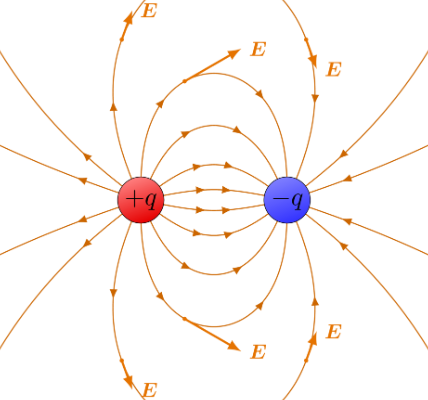
\includegraphics[scale = 0.4]{image/dipolo.png}
    \caption{campo elettromagnetico formato da un dipolo}
    \label{OndeElettrtomagnetiche}
\end{figure}

Se prendessimo un dipolo, insieme di cariche positive e negative bilanciate, e iniziassimo a muoverle esse genererebbero un campo elettrico variabile nel tempo. Dunque in ogni punto si genera un campo magnetico perpendicolare al campo elettrico. Nel caso della Figura \ref{OndeElettrtomagnetiche} ci potremmo immaginare un cerchio che esce dal foglio, e quello rappresenterebbe il campo magnetico, crea un vortice che attraversa il foglio. Questo procedimento si ripete all'infinito ed otteniamo le onde elettromagnetiche mostrate nella seguente Figura.

\begin{figure}[h]
    \centering
    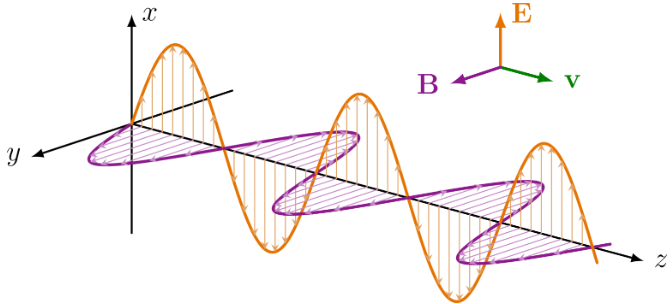
\includegraphics[scale=0.5]{image/ondeElettomagnetiche.png}
    \caption{Propagazione onde elettromagnetiche}
    \label{OndeElettromagentiche}
\end{figure}

Dal punto di vista delle equazioni non c'è un limite di frequenza delle oscillazioni ma tecnologicamente parlando si è arrivati all'ordine dei Gigahertz, un miliardo di oscillazioini al secondo.
\paragraph{}
Ora queste equazioni, per studiare le onde elettromagnetiche, si dovrebbero trasformare in equazioni differenziali perché così guardiamo cosa succede nel singolo punto e non cosa succede nell'insieme.

\section{Equazioni differenziali di Maxwell}

La trasformazione delle equazioni integrali in equazioni differenziali è possibile facendo tendere a zero il volume della superficie chiusa dove è applicato l'integrale.

\begin{equation*}
    \lim_{\Delta v \to 0}  \frac{\oint_s \vec{E} \cdot d\vec{s}}{\Delta v}  = \vec{\nabla}\cdot \vec{E}
\end{equation*}
questo limite ci da la divergenza, uno scalare il quale è la somma di tutte le componenti del gradiente, del campo elettrico. La divergenza di un campo vettoriale è la descrizione matematica
della tendenza del campo a “fuoriuscire” da un punto.

\paragraph{}
In modo analogo si trova l'equazione differenziale lungo una linea chiusa.

\begin{equation*}
    \lim_{\Delta s \to 0}  \frac{\oint_l \vec{E} \cdot d\vec{l}}{\Delta s}  = \vec{\nabla} \times \vec{E}
\end{equation*}

in questo altro caso il limite restituisce il rotore del campo elettrico. Il rotore di un campo vettoriale misura la tendenza del campo a “circolare” attorno a un punto.

\paragraph{}
Dunque le equazioni in forma differenziale diventano:

\begin{equation*}
    1)\vec{\nabla}\cdot \vec{E}  = \frac{\rho}{\varepsilon_0}\qquad3)\,\vec{\nabla} \cdot \vec{B}  = 0
\end{equation*}

\begin{equation*}
    2)\vec{\nabla} \times \vec{E}  = -\frac{d\vec{B}}{dt}\qquad4)\,\vec{\nabla} \times \vec{B}  = \mu_0 \vec{J} + \varepsilon_0\mu_0\frac{d\vec{E}}{dt}
\end{equation*}

\section{Formula di Biot-Savart o prima formula di Laplace}

Questa formula è la sorella della Formula di Coulomb, ma applicata al campo magnetico:

\begin{equation}
    \vec{B} = \frac{\mu_0}{4\pi} \frac{q\vec{v} \times \vec{Ur}}{r^2}
\end{equation}

In un dato punto: 

\begin{equation}
    d\vec{B} = \frac{\mu_0}{4\pi} \frac{i d\vec{l} \times \vec{Ur}}{r^2}
\end{equation}

\section{Filo infinito}

\begin{figure}[H]
    \centering
    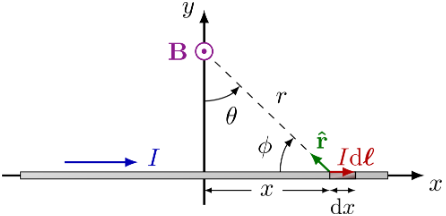
\includegraphics[scale = 0.5]{image/filoInfinitoMagnetico.png}
    \caption{Campo magnetico ad una distanza h dal filo}
    \label{campoMagneticodaUnFiloLeggeBiotSavart}
\end{figure}

\begin{equation}
    d\vec{B} = \frac{\mu_0}{4\pi} \frac{i d\vec{l} \times \vec{Ur}}{r^2}
\end{equation}

Per calcolarlo dobbiamo trasformare tutto in funzione di Theta. Quindi:

\begin{equation*}
    \frac{x}{r} = \tan{\theta}
\end{equation*}
\begin{equation*}
    x = r\tan{\theta}
\end{equation*}
\begin{equation*}
    dx = \frac{r}{\cos^2{\theta}} d\theta
\end{equation*}

\begin{equation*}
    \frac{d}{r} = \cos{\theta}
\end{equation*}
dove $d$ è la distanza dal filo.
\begin{equation*}
    r = \frac{d}{\cos{\theta}}
\end{equation*}

Quindi la formula risulta essere la seguente:

\begin{equation*}
    d\vec{B} = \frac{\mu_0}{4\pi} \frac{i d d\theta \cos{\theta}}{\cos^2{\theta}} \frac{\cos^2{\theta}}{d^2}
\end{equation*}

Semplificando e integrando:

\begin{equation}
    B = \frac{\mu_0 i}{4\pi d}\int_{-\theta} ^{\theta} \cos{\theta} d\theta
\end{equation}

dove $d$ è sempre la distanza tra il punto e il filo. Questo risultato lo avevamo già trovato servendoci della legge di Ampere, infatti se prendiamo $\theta = \frac{\pi}{2}$ avremo proprio:

\begin{equation}
    B = \frac{\mu_0 i}{2 \pi d}\
\end{equation}



Si preferisce usare questa formula perché la legge di Biot-Savart è valida su qualsiasi filo.


\section{Spira}

\begin{figure}[H]
    \centering
    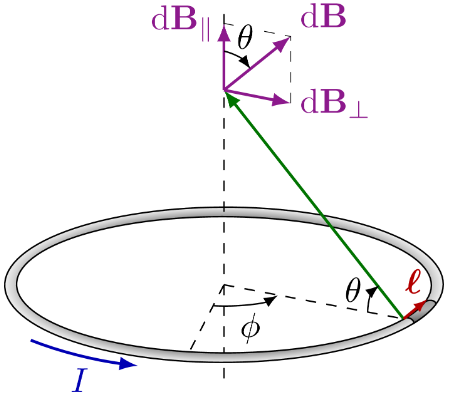
\includegraphics[scale = 0.5]{image/spira.png}
    \caption{Campo magnetico generato da una spira}
    \label{spira}
\end{figure}

\begin{equation}
    B = \frac{\mu_0 i r^2}{2(r^2 + h^2)^{\frac{3}{2}}}
\end{equation}

Dove $r$ risulta essere il raggio e $h$ l'altezza che vi è tra la spira e il punto.

\section{Applicazione della legge di Faraday}

\begin{figure}[H]
    \centering
    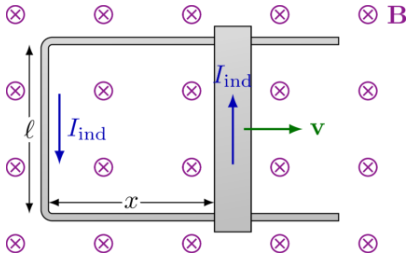
\includegraphics[scale = 0.5]{image/FaradayApplicazione.png}
    \caption{Induzione elettromagnetica}
    \label{FaradayApplicazione}
\end{figure}

Vorremmo calcolare il campo magnetico dell'area compresa tra il filo e la barra.

Per la legge di Faraday calcoliamo facilmente il flusso:

\begin{equation*}
    \oint_l \vec{E} \cdot d\vec{l}  = -\frac{d}{dt}\phi_b
\end{equation*}

dove $\phi_b = Blvt$ 

Derivandola nel tempo troviamo che:

\begin{equation}
    f.e.m.\footnote{f.e.m. = Forza ElettroMotrice, è una differenza di potenziale} = \oint_l \vec{E} \cdot d\vec{l}  = Blv
\end{equation}

L'area sta aumentando quindi il flusso di B sta aumentando, ed esso crea un campo elettrico e dunque una corrente. Tale corrente risulta essere:

\begin{equation*}
    I = \frac{f.e.m}{R}
\end{equation*}

Dove $R$ si intende la resistenza nel circuito.

Questo fenomeno si chiama \textbf{induzione elettromagnetica}.

\section{Legge di Lorentz}
Ogni carica sulla barretta viene spostata con una verta velocità $v$, quindi si genera una forza, concorde al segno della corrente e tale forza risulta essere:

\begin{equation}
    \vec{F} = qvB
\end{equation}

e dunque il lavoro di una forza risulta essere:

\begin{equation}
    L = qvBl
\end{equation}

e il lavoro per unità di carica è:
\begin{equation}
    \frac{L}{q} = Blv
\end{equation}

e risulta essere uguale proprio alla $f.e.m.$.

\section{Induttore}

\begin{figure}[H]
    \centering
    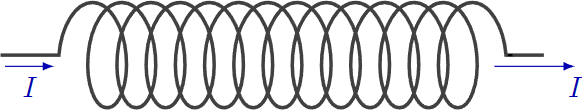
\includegraphics[scale = 0.4]{image/solenoide.png}
    \caption{Induttore}
    \label{Induttore}
\end{figure}

L'induttore è un componente elettrico che genera un campo magnetico al passaggio di corrente elettrica.

Formula principale:

\begin{equation}
    \Delta V = L \frac{dI}{dt}
\end{equation}

Ciò significa che la differenza di potenziale ai capi del solenoide risulta proporzionale ad $L$, l'induttanza, moltiplicato alla derivata nel tempo della corrente, una corrente variabile nel tempo.

Questa relazione può essere dedotta dalle equazioni di base dell'elettromagnetismo grazie alla legge di Ampere, e che abbiamo già dimostrato in precendenza:

\begin{equation}
    B = \frac{\mu_0IN}{l}
\end{equation}

dove $l$ è la lunghezza del solenoide considerato.


Se la corrente I che scorre nel solenoide/induttore è variabile nel tempo, anche B sarà variabile nel tempo. Essendo B variabile nel tempo, si produce una variazione di flusso del campo magnetico concatenato con il solenoide stesso il che produce, per la legge di Faraday, una f.e.m. auto-indotta ai capi dell'induttore, e dunque anche una differenza di potenziale tra una spira e l'altra.

\paragraph{}
Infatti per la legge di Faraday possiamo scrivere che su ogni spira si crea una differenza di potenziale:

\begin{equation*}
    -\frac{d \phi_B}{dt} = El = \Delta V
\end{equation*}
dove $l$ in questo caso è un giro della spira.

per trovare la differenza di potenziale totale, basta moltiplicarlo per il numero di spire $N$:

\begin{equation*}
    \Delta V_{tot} = N \frac{d \phi_B}{dt}
\end{equation*}
\begin{equation*}
    \Delta V_{tot} = N A \frac{\mu_0 N}{l} \frac{d I}{dt} 
\end{equation*}

dove $A$ risulta essere la sezione del tubo, $N$ il numero di spire e $l$ la lunghezza del solenoide.


$A \frac{\mu_0 N}{l}$, viene chiamata auto-induttanza o più semplicemente induttanza e si indica con L.

ecco dimostrato la legge di prima:

\begin{equation}
    \Delta V = \frac{d \phi_B}{dt} = L \frac{d I}{dt} 
    \label{eqSolenoide}
\end{equation}


Il solenoide è un parente stretto del condensatore, infatti oltre alla Equazioni \ref{equazioneCondensatore} e \ref{eqSolenoide}, che legano la corrente e la tensione, possiamo fare un discorso analogo che abbiamo già fatto per il condensatore: vogliamo capire dove va a finire l'energia elettrica che abbiamo usato per caricare l'induttore? Per carica di un induttore significa che si fa passare una corrente ai suoi capi e quando risulta costante allora al suo interno si è creato un campo magnetico costante.

\paragraph{}
Bene questa energia è stipata all'interno del area del solenoide. E da notare che in questo caso non si parla più di energia potenziale, come nel condensatore, ma bensì si parla di energia cinetica. 

\section{Circuito LC}

\begin{figure}[H]
    \centering
    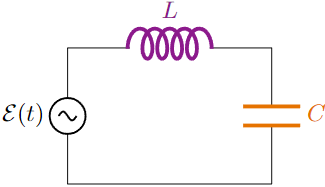
\includegraphics[scale = 0.6]{image/circuito_LC.png}
    \caption{Circuito LC}
    \label{ciruitoLc}
\end{figure}

Se creiamo un circuito formato da un induttore e da una condensatore carico otterremo un circuito risonante, perché il condensatore trasferirà tutta la sua energia, scaricandosi, all'induttore il quale si caricherà e una volta carico inizierà a ridare energia al condensatore e il ciclo riparte. Quindi questo circuito si comporta esattamente come un pendolo.
\paragraph{}
Quindi questo modo permette di creare dei clock, dei timer; ovviamente la corrente si consumerebbe nel tempo, come nel caso del pendolo, infatti si deve mantenere una tensione costante, infatti bisogna inserire anche un generatore il quale vada alla stessa frequenza con cui il circuito oscilla.

\paragraph{}
L'equazione del risonatore è:

\begin{equation}
    LC + \frac{d^2I}{dt^2} + I = 0
\end{equation}

Il risultato di questa equazione differenziale, dopo aver applicato le regole di risoluzione delle equazioni differenziali troviamo il seguente risultato:

\begin{equation}
    I(t) = I_0 \cos{\omega t}\qquad\omega = \frac{1}{\sqrt{LC}}
\end{equation}

Ovvero una corrente oscillante nel tempo.
